% !TeX program = lualatex
% !TeX encoding = utf8
% !TeX spellcheck = english
% !TeX version = 2020
%
% **************************************************
% Document Class Definition
% **************************************************
% B5->9pt
\documentclass[%
    paper=A4,               % paper size --> A4 is default in Germany
    twoside=false,          % onesite or twoside printing TODO: true
    openright,              % doublepage cleaning ends up right side
    parskip=half,           % spacing value / method for paragraphs
    chapterprefix=true,     % prefix for chapter marks
    11pt,                   % font size
    headings=normal,        % size of headings
    bibliography=totoc,     % include bib in toc
    listof=totoc,           % include listof entries in toc
    titlepage=on,           % own page for each title page
    captions=tableabove,    % display table captions above the float env
    chapterprefix=false,    % do not display a prefix for chapters
    appendixprefix=false,   % but display a prefix for appendix chapter
    draft=false,            % value for draft version
]{scrreprt}%
%
%
% **************************************************
% Setup YOUR thesis document in this file !
% **************************************************
% !TEX root = thesis.tex
%
\usepackage{iftex}
% **************************************************
% Files' Character Encoding
% **************************************************
\ifPDFTeX
    \usepackage[utf8]{inputenc}
\fi
%
% **************************************************
% Information and Commands for Reuse
% **************************************************
\newcommand{\thesisTitle}{Nerve Fiber Modelling and 3D-PLI Simulations:\\ A Fiber Architect Simulation Toolbox} %Modelling of 3D Nerve Fibers and their Applications in 3D-PLI
\newcommand{\thesisName}{Felix Matuschke}
\newcommand{\thesisSubject}{Documentation}
\newcommand{\thesisDate}{\today}
\newcommand{\thesisVersion}{My First Draft}
%
\newcommand{\thesisFirstReviewer}{Prof. Dr. Gunnar Schr\"{o}der}
\newcommand{\thesisFirstReviewerUniversity}{\protect{IBI-7}}
\newcommand{\thesisFirstReviewerDepartment}{Forschungszentrum J\"{u}lich}
%
\newcommand{\thesisSecondReviewer}{Prof. Dr. Katrin Amunts}
\newcommand{\thesisSecondReviewerUniversity}{\protect{INM-1}}
\newcommand{\thesisSecondReviewerDepartment}{Forschungszentrum J\"{u}lich}
%
\newcommand{\thesisFirstSupervisor}{Prof. Dr. Markus Axer}
\newcommand{\thesisFirstSupervisorUniversity}{\protect{INM-1}}
\newcommand{\thesisFirstSupervisorDepartment}{Forschungszentrum J\"{u}lich}
%
\newcommand{\thesisUniversity}{\protect{Heinrich-Heine-Universit\"{a}t D\"{u}sseldorf}}
\newcommand{\thesisUniversityDepartment}{Math.-Nat. Fakult\"{a}t}
\newcommand{\thesisUniversityInstitute}{}
\newcommand{\thesisUniversityGroup}{}
\newcommand{\thesisUniversityCity}{D\"{u}sseldorf}
\newcommand{\thesisUniversityStreetAddress}{Universitt\"{a}sstra{\ss}e 1}
\newcommand{\thesisUniversityPostalCode}{40225 D\"{u}sseldorf}
% 
\newcommand{\thesisInstitute}{\protect{Forschungszentrum J\"{u}lich}}
\newcommand{\thesisInstituteDepartment}{Institut für Neurowissenschaften und Medizin}
\newcommand{\thesisInstituteInstitute}{Strukturelle und funktionelle Organisation des Gehirns (INM-1)}
\newcommand{\thesisInstituteGroup}{Faserbahnarchitektur}
\newcommand{\thesisInstituteCity}{J\"{u}lich}
\newcommand{\thesisInstituteStreetAddress}{Wilhelm-Johnen-Stra{\ss}e}
\newcommand{\thesisInstitutePostalCode}{52428 J\"{u}lich}
%
% **************************************************
% Debug LaTeX Information
% **************************************************
\usepackage{silence}
% \WarningFilter[references]{latex} {There were undefined references}
\WarningFilter[references]{latex} {Reference }
% \listfiles
% 
% **************************************************
% User Commands
% **************************************************
% 
% \makeatletter
% \renewcommand\listoftables{%
%         \@starttoc{lot}%
% }
% \makeatother
% % 
% \makeatletter
% \renewcommand\listoffigures{%
%         \@starttoc{lof}%
% }
% \makeatother
% % 
% \makeatletter
% \renewcommand\lstlistoflistings{%
%         \@starttoc{lof}%
% }
% \makeatother
%
%
% **************************************************
% Pre cleanthesis imports
% **************************************************
\RequirePackage[dvipsnames]{xcolor}
\usepackage{tikz}
% 
% **************************************************
% Load and Configure Packages
% **************************************************
\usepackage[english]{babel} % babel system, adjust the language of the content
\PassOptionsToPackage{% setup clean thesis style
    figuresep=colon,%
    hangfigurecaption=false,%
    hangsection=true,%
    hangsubsection=true,%
    sansserif=true,%
    configurelistings=true,%
    colorize=full,%
    colortheme=bluemagenta,%
    configurebiblatex=true,%
    bibsys=biber,%
    bibfile=bib-refs,%
    bibstyle=alphabetic,%
    bibsorting=nty,%
}{cleanthesis}
\usepackage{cleanthesis}
%
% \colorlet{citeColor}{green!50!black}
% \colorlet{linkColor}{green!75!black>wheel,1,2}
% \colorlet{urlColor}{green!75!black>twheel,1,2}
\colorlet{citeColor}{violet>twheel,2,3}
\colorlet{linkColor}{violet}
\colorlet{urlColor}{violet>twheel,1,3}
% 
\hypersetup{% setup the hyperref-package options
    pdftitle={\thesisTitle},    %   - title (PDF meta)
    pdfsubject={\thesisSubject},%   - subject (PDF meta)
    pdfauthor={\thesisName},    %   - author (PDF meta)
    plainpages=false,           %   -
    colorlinks=true,            %   - colorize links?
    pdfborder={0 0 0},          %   -
    breaklinks=true,            %   - allow line break inside links
    bookmarksnumbered=true,     %
    bookmarksopen=true,         %
    citecolor=citeColor,        %
    linkcolor=linkColor,        %
    urlcolor=urlColor,          %
}
%
% **************************************************
%  Packages
% **************************************************
\usepackage{scrhack}
\usepackage{float}              % [H]
\usepackage{graphicx}           % (pdf, png, jpg, eps)
\usepackage[export]{adjustbox}
\usepackage{pdfpages}
\usepackage{subcaption}
\usepackage{minitoc}
\usepackage{tcolorbox}
\usepackage{enumitem}
% 
\usepackage{amsmath, amssymb, amsthm, mathtools}
\ifPDFTeX
    % \usepackage{newtxsf} ???
    \usepackage{newtxmath} % new math fonts\usepackage[libertine, vvarbb]{newtxmath}
    
\else
    \usepackage{fontspec}
    \usepackage[warnings-off={mathtools-colon,mathtools-overbracket}]{unicode-math}
    \usepackage{lualatex-math}
    \setmathfont{Latin Modern Math}
\fi
% 
\usepackage{dirtree}
\usepackage[bottom]{footmisc}
% 
\usepackage{siunitx} 
\usepackage{upgreek}
\sisetup{
        detect-mode=true,detect-family=false,
        detect-display-math=false,detect-shape=false,
        list-units=brackets, range-units=brackets,
        list-final-separator = {,},
        list-pair-separator={,},
        % list-pair-separator={\text{~and~}},
        range-phrase = {\text{~to~}},
        math-micro=µ,
        binary-units = true
        } %\mathrm{\mu}} %math-micro=\muup,
% \DeclareSIUnit{\arbitraryunit}{\mathit{arb. unit}}
% \DeclareSIUnit\steps{steps}
% \DeclareSIUnit\cpus{cpus}
% \AtBeginDocument{\sisetup{math-rm=\mathrm, text-rm=\sffamily}}
% 
% \usepackage{caption}
\usepackage[nameinlink]{cleveref}
% \usepackage{esvect} % see \let\vv\mathbf
% 
\usepackage{currfile}
\usepackage{blindtext}
%\usepackage{ifplatform}
\usepackage{mwe}
\usepackage{acro}
\usepackage{dirtytalk}
% \usepackage{stackengine}    % for double sided floats
\usepackage{pdflscape}
\usepackage{rotating}         
\newsavebox{\largestimage}    
\newsavebox{\newtable}
% 
\acsetup{barriers/use=true,barriers/reset = true}
% 
% \crefname{figure}{fig.}{fig.}
% \Crefname{figure}{Fig.}{Fig.}
% 
\makeatletter
\def\convertto#1#2{\strip@pt\dimexpr #2*65536/\number\dimexpr 1#1}
\makeatother
% 
\newcommand{\fakesection}[1]{%
  \par\refstepcounter{section}% Increase section counter
  \sectionmark{#1}% Add section mark (header)
  \addcontentsline{toc}{section}{\protect\numberline{\thesection}#1}% Add section to ToC
  % Add more content here, if needed.
}
% 
% **************************************************
%  Minitoc
% **************************************************
\renewcommand*{\partheadstartvskip}{%
  \null\vskip20pt
}
\renewcommand*{\partheadendvskip}{%
  \vskip2pt
}
\renewcommand\beforeparttoc{}
\let\oldparttoc\parttoc
\renewcommand*{\parttoc}{{\hypersetup{hidelinks}\oldparttoc}}
% 
% **************************************************
%  Math
% **************************************************
% \AtBeginDocument{\renewcommand{\minus}{\scalebox{0.75}[1.0]{$-$}}} % different height than -
\AtBeginDocument{\renewcommand{\vec}[1]{\mathbf{#1}}}
\newcommand{\mat}[1]{\mathcal{#1}}
\newcommand{\topbar}[1]{\mkern 1.5mu\overline{\mkern-1.5mu#1\mkern-1.5mu}\mkern 1.5mu}
% \usepackage{MnSymbol} defines to many math symbols for pdflatex
\DeclarePairedDelimiter\abs{\lvert}{\rvert}
\DeclarePairedDelimiter\norm{\lVert}{\rVert}
\DeclarePairedDelimiter\ceil{\lceil}{\rceil}
\DeclarePairedDelimiter\floor{\lfloor}{\rfloor}
\DeclareMathOperator{\atantwo}{atan2}
\DeclareMathOperator{\divergence}{div}
\DeclareMathOperator{\gauss}{normal}
\AtBeginDocument{\newcommand{\integer}[1]{\textnormal{$\mathrm{int}$}}}
\AtBeginDocument{\newcommand{\round}[1]{\textnormal{$\mathrm{round}$}}}
%
% **************************************************
% Syntax Highlighting
% **************************************************
\usepackage{listings}
% 
\newfloat{lstfloat}{htbp}{lop}
\floatname{lstfloat}{Alg.}
\crefname{lstfloat}{alg.}{alg.}
\Crefname{lstfloat}{Alg.}{Alg.}
\crefname{pluralequation}{eqs.}{eqs.}
\renewcommand{\lstlistingname}{Alg.}
\renewcommand{\lstlistlistingname}{List of Algorithm}
% 
\definecolor{syntax_red}{RGB}{160,0,0}
\definecolor{syntax_green}{RGB}{0,160,0}
\definecolor{syntax_blue}{RGB}{0,0,210}
\definecolor{syntax_mauve}{RGB}{150,0,210}
\definecolor{syntax_keywords}{RGB}{255,0,90}
\definecolor{syntax_comments}{RGB}{0,0,113}
%
% 
\lstdefinestyle{common}{
    basicstyle=\footnotesize\ttfamily,
    showstringspaces=false,
    breaklines=false,
    captionpos=b,
    frame=tb,
    xleftmargin=\parindent,
}
% 
\lstdefinestyle{cpp}{
    language=C++,
    style=common,
    keywordstyle=\color{syntax_blue},
    commentstyle=\color{syntax_green},
    stringstyle=\color{syntax_red},
    % identifierstyle=\color{syntax_mauve},
    tabsize=2,
}
%  
\lstdefinestyle{python}{
    language=Python, 
    style=common,
    keywordstyle=\color{syntax_blue},
    commentstyle=\color{syntax_green},
    stringstyle=\color{syntax_red},
    % identifierstyle=\color{syntax_green},
    % procnamekeys={def,class},
	tabsize=3,
}
% 
% Hyphenate code
\usepackage[htt]{hyphenat}
% 
\newcommand{\breakingperiod}{%
  \penalty0 % allow a break before the period
  .\nobreak\hspace{0pt}%
}
% 
\ExplSyntaxOn
% 
\NewDocumentCommand{\code}{m}
 {
  \texttt
   {
    \seq_set_split:Nnn \l_michael_lw_seq { . } { #1 }
    \seq_use:Nn \l_michael_lw_seq { \breakingperiod }
   }
 }
% 
\ExplSyntaxOff
%
% **************************************************
% Tikz & PGFplots
% **************************************************
\usepackage{shellesc}
% \usepackage{tikz} before hyperref
\usepackage{tikz-3dplot}
\usetikzlibrary{math}
\usetikzlibrary{shapes, arrows}
\usetikzlibrary{mindmap, backgrounds}
\usetikzlibrary{calc}
\usetikzlibrary{intersections}
\usetikzlibrary{perspective}
\usetikzlibrary{3d}
\usetikzlibrary{arrows.meta}
\usetikzlibrary{patterns}
\usetikzlibrary{bending} % bend arrow heads
\usetikzlibrary{decorations.pathreplacing}
\tikzset{>=latex}
% 
% \usepackage{pdftexcmds} % for hased externalized names
% \makeatletter
% \ifx\pdf@filemdfivesum\undefined\def\pdf@filemdfivesum#{\mdfivesum file}\fi
% \let\filesum\pdf@filemdfivesum
% \makeatother
%
\usepackage{pgfplots}
\pgfplotsset{compat=1.17}
\usepgfplotslibrary{polar}
\usepgfplotslibrary{colorbrewer}
\usepgfplotslibrary{statistics}
\usepgfplotslibrary{groupplots}
\usepgfplotslibrary{patchplots}
\usepgfplotslibrary{colormaps}
\usepgfplotslibrary{fillbetween}
\usepackage{booktabs,colortbl}
\usepackage{multirow}
%
% 3d canvis
\makeatletter
\tikzoption{canvas is plane}[]{\@setOxy#1}
\def\@setOxy O(#1,#2,#3)x(#4,#5,#6)y(#7,#8,#9)%
  {\def\tikz@plane@origin{\pgfpointxyz{#1}{#2}{#3}}%
   \def\tikz@plane@x{\pgfpointxyz{#4}{#5}{#6}}%
   \def\tikz@plane@y{\pgfpointxyz{#7}{#8}{#9}}%
   \tikz@canvas@is@plane
  }
\makeatother 
% 
\newlength{\tikzwidth}
\newlength{\tikzheight}
\setlength{\tikzwidth}{\textwidth} %13.87303cm
\setlength{\tikzheight}{\textheight} %22.37076cm
% 
\makeatletter
\newcommand{\inputtikzext}[1]{%
	% \IfFileExists{#1.tikz}{
		\input{#1.tikz}
	% }{
  %   \@latex@warning{.....#1.tikz..... not found. Using example-image.}
	% 	\noindent\includegraphics[width=\tikzwidth]{example-image}
	% }
}
\makeatother
% 
\makeatletter
\newcommand{\inputtikz}[2][false]{%
    % \ifthenelse{\boolean{#1}}{
        \inputtikzext{#2}
%     }{
% 	\IfFileExists{tikz/#2.pdf}{% check if pdf tikz/.../*.pdf exists
% 		\includegraphics{tikz/#2.pdf}
% 	}{ % build ext tikz
% 		\inputtikzext{#2}
% 	}}
}
\makeatother
% 
\usepackage{environ}
\makeatletter
\newsavebox{\measure@tikzpicture}
\NewEnviron{tikzsize}[3][true]{%
	\def\tikzscale{1}%
	\ifthenelse{\boolean{#1}}{
	\tikzifexternalizingnext{%
		\begin{lrbox}{\measure@tikzpicture}%
		\tikzset{external/export next=false,external/optimize=false}% force translation of this BODY (and do not optimize it away as it would usually do):
		\BODY
		\end{lrbox}%
		\expandafter\pgfmathparse{#2/\wd\measure@tikzpicture}%
		\edef\tikzscalewidth{\pgfmathresult}%
		\expandafter\pgfmathparse{#3/\ht\measure@tikzpicture}%
		\edef\tikzscaleheight{\pgfmathresult}%
		\pgfmathparse{min(\tikzscalewidth, \tikzscaleheight)}%
		\edef\tikzscale{\pgfmathresult}%
		\BODY
	}{% this will re-use an existing external graphics:
		\BODY
	}}{
	    \begin{lrbox}{\measure@tikzpicture}%
		\tikzset{external/export next=false,external/optimize=false}% force translation of this BODY (and do not optimize it away as it would usually do):
		\BODY
		\end{lrbox}%
		\expandafter\pgfmathparse{#2/\wd\measure@tikzpicture}%
		\edef\tikzscalewidth{\pgfmathresult}%
		\expandafter\pgfmathparse{#3/\ht\measure@tikzpicture}%
		\edef\tikzscaleheight{\pgfmathresult}%
		\pgfmathparse{min(\tikzscalewidth, \tikzscaleheight)}%
		\edef\tikzscale{\pgfmathresult}%
		\BODY
	}
}
\makeatother
% 
% **************************************************
% PGFplotsTable
% **************************************************
\usepackage{pgfplotstable}
\usepackage{array,multirow,makecell}
\newcolumntype{R}[1]{>{\raggedleft\arraybackslash }b{#1}}
\newcolumntype{L}[1]{>{\raggedright\arraybackslash }b{#1}}
\newcolumntype{C}[1]{>{\centering\arraybackslash }b{#1}}
% 
% \captionsetup[table]{textfont=it, parskip=10em} % skip does not work for table
\pgfplotstableset{thesisTableStyle/.style={
    every even row/.style={before row={\rowcolor[gray]{0.90}}},
    % empty cells with={--}, % replace empty cells with '--'
    every head row/.style={before row=\toprule,after row=\midrule},
    every last row/.style={after row=\bottomrule},
}}
% 
\pgfplotstableset{
    rowbf/.style={
        postproc cell content/.append code={
          \count0=\pgfplotstablerow
            \advance\count0 by1
            \ifnum\count0=#1
              \pgfkeysalso{@cell content=\textbf{##1}}%
            \fi
        },
    },
}
\pgfplotstableset{
    rowem/.style={
        postproc cell content/.append code={
          \count0=\pgfplotstablerow
            \advance\count0 by1
            \ifnum\count0=#1
              \pgfkeysalso{@cell content=\emph{##1}}%
            \fi
        },
    },
}
% 
% every row 3 column 3/.style={postproc cell content/.style=
%         {@cell content=\textbf{##1}}}
% 
% **************************************************
% User Macros
% **************************************************
\newcommand{\tu}{\textunderscore}
\newcommand{\note}[1]{\textcolor{gray}{\textit{#1}}}
\newcommand{\dummy}[2][...]{\textcolor{blue!75!white}{\textbf{\{#1\}}}}
% 
\usepackage[colorinlistoftodos,prependcaption,textsize=footnotesize]{todonotes}
\newlength{\itodolength}
\setlength{\itodolength}{\textwidth minus 2.1411pt}
\presetkeys%
    {todonotes}%
    {backgroundcolor=ProcessBlue,
     linecolor=ProcessBlue,
     inlinewidth=\itodolength,
     tickmarkheight=1ex}{} %
\makeatletter
\renewcommand{\todo}[2][]{%
  {\tikzset{external/export=false}\@todo[#1]{#2}}%
}
\makeatother
\reversemarginpar
\setlength{\marginparwidth}{4cm}
\newcommand{\itodo}[2][]{\todo[inline, #1]{#2}}
\newcommand{\TODO}[2][]{\todo[color=red, #1]{#2}}
\newcommand{\ITODO}[2][]{\todo[inline, color=red, #1]{#2}}
\newcommand{\markus}[1]{\textcolor{orange!90!black}{#1}}
\newcommand{\fixme}[1]{\textcolor{red!75!black}{\textbf{#1}}}
% \newcommand{\markus}[1]{\todo[color=orange]{#1}}
% \newcommand{\imarkus}[1]{\todo[inline, color=orange]{#1}}
% 
% **************************************************
% Debug LaTeX Information
% **************************************************
% \usepackage{showframe}
% 
% **************************************************
% Custom Colors
% **************************************************
%  from colorbrewer
\pgfplotsset{cycle list/Dark2}
% 
\definecolor{set11}{HTML}{e41a1c}
\definecolor{set12}{HTML}{377eb8}
\definecolor{set13}{HTML}{4daf4a}
\definecolor{set14}{HTML}{984ea3}
\definecolor{set15}{HTML}{ff7f00}
\definecolor{set16}{HTML}{ffff33}
\definecolor{set17}{HTML}{a65628}
\definecolor{set18}{HTML}{f781bf}
% 
\definecolor{set21}{HTML}{66c2a5}
\definecolor{set22}{HTML}{fc8d62}
\definecolor{set23}{HTML}{8da0cb}
\definecolor{set24}{HTML}{e78ac3}
\definecolor{set25}{HTML}{a6d854}
\definecolor{set26}{HTML}{ffd92f}
\definecolor{set27}{HTML}{e5c494}
\definecolor{set28}{HTML}{b3b3b3}
% 
\definecolor{dark21}{HTML}{1b9e77}
\definecolor{dark22}{HTML}{d95f02}
\definecolor{dark23}{HTML}{7570b3}
\definecolor{dark24}{HTML}{e7298a}
\definecolor{dark25}{HTML}{66a61e}
\definecolor{dark26}{HTML}{e6ab02}
\definecolor{dark27}{HTML}{a6761d}
\definecolor{dark28}{HTML}{666666}
% 
\colorlet{sred}{set11}
\colorlet{sgreen}{set13}
\colorlet{sblue}{set12}
% 
\colorlet{dred}{dark22}
\colorlet{dgreen}{dark21}
\colorlet{dblue}{dark23} 
% 
\colorlet{RED}{dark22}
\colorlet{GREEN}{dark21}
\colorlet{BLUE}{dark23} 
% 
% \makeatletter
% \definecolor{cc21}{HTML}{A6CEE3}
% \definecolor{cc22}{HTML}{1F78B4}
% \pgfplotscreateplotcyclelist{cc2}{cc21, cc22}
% \makeatother
% 
\pgfplotsset{
   /pgfplots/colormap={cividis}{%
      rgb=(0.00000000, 0.13511200, 0.30475100)
      rgb=(0.00000000, 0.13806800, 0.31110500)
      rgb=(0.00000000, 0.14101300, 0.31757900)
      rgb=(0.00000000, 0.14395100, 0.32398200)
      rgb=(0.00000000, 0.14687700, 0.33047900)
      rgb=(0.00000000, 0.14979100, 0.33706500)
      rgb=(0.00000000, 0.15267300, 0.34370400)
      rgb=(0.00000000, 0.15537700, 0.35050000)
      rgb=(0.00000000, 0.15793200, 0.35752100)
      rgb=(0.00000000, 0.16049500, 0.36453400)
      rgb=(0.00000000, 0.16305800, 0.37160800)
      rgb=(0.00000000, 0.16562100, 0.37876900)
      rgb=(0.00000000, 0.16820400, 0.38590200)
      rgb=(0.00000000, 0.17080000, 0.39310000)
      rgb=(0.00000000, 0.17342000, 0.40035300)
      rgb=(0.00000000, 0.17608200, 0.40757700)
      rgb=(0.00000000, 0.17880200, 0.41476400)
      rgb=(0.00000000, 0.18161000, 0.42185900)
      rgb=(0.00000000, 0.18455000, 0.42880200)
      rgb=(0.00000000, 0.18691500, 0.43553200)
      rgb=(0.00000000, 0.18876900, 0.43956300)
      rgb=(0.00000000, 0.19095000, 0.44108500)
      rgb=(0.00000000, 0.19336600, 0.44156100)
      rgb=(0.00360200, 0.19591100, 0.44156400)
      rgb=(0.01785200, 0.19852800, 0.44124800)
      rgb=(0.03211000, 0.20119900, 0.44078500)
      rgb=(0.04620500, 0.20390300, 0.44019600)
      rgb=(0.05837800, 0.20662900, 0.43953100)
      rgb=(0.06896800, 0.20937200, 0.43886300)
      rgb=(0.07862400, 0.21212200, 0.43810500)
      rgb=(0.08746500, 0.21487900, 0.43734200)
      rgb=(0.09564500, 0.21764300, 0.43659300)
      rgb=(0.10340100, 0.22040600, 0.43579000)
      rgb=(0.11065800, 0.22317000, 0.43506700)
      rgb=(0.11761200, 0.22593500, 0.43430800)
      rgb=(0.12429100, 0.22869700, 0.43354700)
      rgb=(0.13066900, 0.23145800, 0.43284000)
      rgb=(0.13683000, 0.23421600, 0.43214800)
      rgb=(0.14285200, 0.23697200, 0.43140400)
      rgb=(0.14863800, 0.23972400, 0.43075200)
      rgb=(0.15426100, 0.24247500, 0.43012000)
      rgb=(0.15973300, 0.24522100, 0.42952800)
      rgb=(0.16511300, 0.24796500, 0.42890800)
      rgb=(0.17036200, 0.25070700, 0.42832500)
      rgb=(0.17549000, 0.25344400, 0.42779000)
      rgb=(0.18050300, 0.25618000, 0.42729900)
      rgb=(0.18545300, 0.25891400, 0.42678800)
      rgb=(0.19030300, 0.26164400, 0.42632900)
      rgb=(0.19505700, 0.26437200, 0.42592400)
      rgb=(0.19976400, 0.26709900, 0.42549700)
      rgb=(0.20438500, 0.26982300, 0.42512600)
      rgb=(0.20892600, 0.27254600, 0.42480900)
      rgb=(0.21343100, 0.27526600, 0.42448000)
      rgb=(0.21786300, 0.27798500, 0.42420600)
      rgb=(0.22226400, 0.28070200, 0.42391400)
      rgb=(0.22659800, 0.28341900, 0.42367800)
      rgb=(0.23087100, 0.28613400, 0.42349800)
      rgb=(0.23512000, 0.28884800, 0.42330400)
      rgb=(0.23931200, 0.29156200, 0.42316700)
      rgb=(0.24348500, 0.29427400, 0.42301400)
      rgb=(0.24760500, 0.29698600, 0.42291700)
      rgb=(0.25167500, 0.29969800, 0.42287300)
      rgb=(0.25573100, 0.30240900, 0.42281400)
      rgb=(0.25974000, 0.30512000, 0.42281000)
      rgb=(0.26373800, 0.30783100, 0.42278900)
      rgb=(0.26769300, 0.31054200, 0.42282100)
      rgb=(0.27163900, 0.31325300, 0.42283700)
      rgb=(0.27551300, 0.31596500, 0.42297900)
      rgb=(0.27941100, 0.31867700, 0.42303100)
      rgb=(0.28324000, 0.32139000, 0.42321100)
      rgb=(0.28706500, 0.32410300, 0.42337300)
      rgb=(0.29088400, 0.32681600, 0.42351700)
      rgb=(0.29466900, 0.32953100, 0.42371600)
      rgb=(0.29842100, 0.33224700, 0.42397300)
      rgb=(0.30216900, 0.33496300, 0.42421300)
      rgb=(0.30588600, 0.33768100, 0.42451200)
      rgb=(0.30960100, 0.34039900, 0.42479000)
      rgb=(0.31328700, 0.34312000, 0.42512000)
      rgb=(0.31694100, 0.34584200, 0.42551200)
      rgb=(0.32059500, 0.34856500, 0.42588900)
      rgb=(0.32425000, 0.35128900, 0.42625000)
      rgb=(0.32787500, 0.35401600, 0.42667000)
      rgb=(0.33147400, 0.35674400, 0.42714400)
      rgb=(0.33507300, 0.35947400, 0.42760500)
      rgb=(0.33867300, 0.36220600, 0.42805300)
      rgb=(0.34224600, 0.36493900, 0.42855900)
      rgb=(0.34579300, 0.36767600, 0.42912700)
      rgb=(0.34934100, 0.37041400, 0.42968500)
      rgb=(0.35289200, 0.37315300, 0.43022600)
      rgb=(0.35641800, 0.37589600, 0.43082300)
      rgb=(0.35991600, 0.37864100, 0.43150100)
      rgb=(0.36344600, 0.38138800, 0.43207500)
      rgb=(0.36692300, 0.38413900, 0.43279600)
      rgb=(0.37043000, 0.38689000, 0.43342800)
      rgb=(0.37388400, 0.38964600, 0.43420900)
      rgb=(0.37737100, 0.39240400, 0.43489000)
      rgb=(0.38083000, 0.39516400, 0.43565300)
      rgb=(0.38426800, 0.39792800, 0.43647500)
      rgb=(0.38770500, 0.40069400, 0.43730500)
      rgb=(0.39115100, 0.40346400, 0.43809600)
      rgb=(0.39456800, 0.40623600, 0.43898600)
      rgb=(0.39799100, 0.40901100, 0.43984800)
      rgb=(0.40141800, 0.41179000, 0.44070800)
      rgb=(0.40482000, 0.41457200, 0.44164200)
      rgb=(0.40822600, 0.41735700, 0.44257000)
      rgb=(0.41160700, 0.42014500, 0.44357700)
      rgb=(0.41499200, 0.42293700, 0.44457800)
      rgb=(0.41838300, 0.42573300, 0.44556000)
      rgb=(0.42174800, 0.42853100, 0.44664000)
      rgb=(0.42512000, 0.43133400, 0.44769200)
      rgb=(0.42846200, 0.43414000, 0.44886400)
      rgb=(0.43181700, 0.43695000, 0.44998200)
      rgb=(0.43516800, 0.43976300, 0.45113400)
      rgb=(0.43850400, 0.44258000, 0.45234100)
      rgb=(0.44181000, 0.44540200, 0.45365900)
      rgb=(0.44514800, 0.44822600, 0.45488500)
      rgb=(0.44844700, 0.45105300, 0.45626400)
      rgb=(0.45175900, 0.45388700, 0.45758200)
      rgb=(0.45507200, 0.45671800, 0.45897600)
      rgb=(0.45836600, 0.45955200, 0.46045700)
      rgb=(0.46161600, 0.46240500, 0.46196900)
      rgb=(0.46494700, 0.46524100, 0.46339500)
      rgb=(0.46825400, 0.46808300, 0.46490800)
      rgb=(0.47150100, 0.47096000, 0.46635700)
      rgb=(0.47481200, 0.47383200, 0.46768100)
      rgb=(0.47818600, 0.47669900, 0.46884500)
      rgb=(0.48162200, 0.47957300, 0.46976700)
      rgb=(0.48514100, 0.48245100, 0.47038400)
      rgb=(0.48869700, 0.48531800, 0.47100800)
      rgb=(0.49227800, 0.48819800, 0.47145300)
      rgb=(0.49591300, 0.49107600, 0.47175100)
      rgb=(0.49955200, 0.49396000, 0.47203200)
      rgb=(0.50318500, 0.49685100, 0.47230500)
      rgb=(0.50686600, 0.49974300, 0.47243200)
      rgb=(0.51054000, 0.50264300, 0.47255000)
      rgb=(0.51422600, 0.50554600, 0.47264000)
      rgb=(0.51792000, 0.50845400, 0.47270700)
      rgb=(0.52164300, 0.51136700, 0.47263900)
      rgb=(0.52534800, 0.51428500, 0.47266000)
      rgb=(0.52908600, 0.51720700, 0.47254300)
      rgb=(0.53282900, 0.52013500, 0.47240100)
      rgb=(0.53655300, 0.52306700, 0.47235200)
      rgb=(0.54030700, 0.52600500, 0.47216300)
      rgb=(0.54406900, 0.52894800, 0.47194700)
      rgb=(0.54784000, 0.53189500, 0.47170400)
      rgb=(0.55161200, 0.53484900, 0.47143900)
      rgb=(0.55539300, 0.53780700, 0.47114700)
      rgb=(0.55918100, 0.54077100, 0.47082900)
      rgb=(0.56297200, 0.54374100, 0.47048800)
      rgb=(0.56680200, 0.54671500, 0.46998800)
      rgb=(0.57060700, 0.54969500, 0.46959300)
      rgb=(0.57441700, 0.55268200, 0.46917200)
      rgb=(0.57823600, 0.55567300, 0.46872400)
      rgb=(0.58208700, 0.55867000, 0.46811800)
      rgb=(0.58591600, 0.56167400, 0.46761800)
      rgb=(0.58975300, 0.56468200, 0.46709000)
      rgb=(0.59362200, 0.56769700, 0.46640100)
      rgb=(0.59746900, 0.57071800, 0.46582100)
      rgb=(0.60135400, 0.57374300, 0.46507400)
      rgb=(0.60521100, 0.57677700, 0.46444100)
      rgb=(0.60910500, 0.57981600, 0.46363800)
      rgb=(0.61297700, 0.58286100, 0.46295000)
      rgb=(0.61685200, 0.58591300, 0.46223700)
      rgb=(0.62076500, 0.58897000, 0.46135100)
      rgb=(0.62465400, 0.59203400, 0.46058300)
      rgb=(0.62857600, 0.59510400, 0.45964100)
      rgb=(0.63250600, 0.59818000, 0.45866800)
      rgb=(0.63641200, 0.60126400, 0.45781800)
      rgb=(0.64035200, 0.60435400, 0.45679100)
      rgb=(0.64427000, 0.60745000, 0.45588600)
      rgb=(0.64822200, 0.61055300, 0.45480100)
      rgb=(0.65217800, 0.61366400, 0.45368900)
      rgb=(0.65611400, 0.61678000, 0.45270200)
      rgb=(0.66008200, 0.61990400, 0.45153400)
      rgb=(0.66405500, 0.62303400, 0.45033800)
      rgb=(0.66800800, 0.62617100, 0.44927000)
      rgb=(0.67199100, 0.62931600, 0.44801800)
      rgb=(0.67598100, 0.63246800, 0.44673600)
      rgb=(0.67997900, 0.63562600, 0.44542400)
      rgb=(0.68395000, 0.63879300, 0.44425100)
      rgb=(0.68795700, 0.64196600, 0.44288600)
      rgb=(0.69197100, 0.64514500, 0.44149100)
      rgb=(0.69598500, 0.64833400, 0.44007200)
      rgb=(0.70000800, 0.65152900, 0.43862400)
      rgb=(0.70403700, 0.65473100, 0.43714700)
      rgb=(0.70806700, 0.65794200, 0.43564700)
      rgb=(0.71210500, 0.66116000, 0.43411700)
      rgb=(0.71617700, 0.66438400, 0.43238600)
      rgb=(0.72022200, 0.66761800, 0.43080500)
      rgb=(0.72427400, 0.67085900, 0.42919400)
      rgb=(0.72833400, 0.67410700, 0.42755400)
      rgb=(0.73242200, 0.67736400, 0.42571700)
      rgb=(0.73648800, 0.68062900, 0.42402800)
      rgb=(0.74058900, 0.68390000, 0.42213100)
      rgb=(0.74466400, 0.68718100, 0.42039300)
      rgb=(0.74877200, 0.69047000, 0.41844800)
      rgb=(0.75288600, 0.69376600, 0.41647200)
      rgb=(0.75697500, 0.69707100, 0.41465900)
      rgb=(0.76109600, 0.70038400, 0.41263800)
      rgb=(0.76522300, 0.70370500, 0.41058700)
      rgb=(0.76935300, 0.70703500, 0.40851600)
      rgb=(0.77348600, 0.71037300, 0.40642200)
      rgb=(0.77765100, 0.71371900, 0.40411200)
      rgb=(0.78179500, 0.71707400, 0.40196600)
      rgb=(0.78596500, 0.72043800, 0.39961300)
      rgb=(0.79011600, 0.72381000, 0.39742300)
      rgb=(0.79429800, 0.72719000, 0.39501600)
      rgb=(0.79848000, 0.73058000, 0.39259700)
      rgb=(0.80266700, 0.73397800, 0.39015300)
      rgb=(0.80685900, 0.73738500, 0.38768400)
      rgb=(0.81105400, 0.74080100, 0.38519800)
      rgb=(0.81527400, 0.74422600, 0.38250400)
      rgb=(0.81949900, 0.74765900, 0.37978500)
      rgb=(0.82372900, 0.75110100, 0.37704300)
      rgb=(0.82795900, 0.75455300, 0.37429200)
      rgb=(0.83219200, 0.75801400, 0.37152900)
      rgb=(0.83642900, 0.76148300, 0.36874700)
      rgb=(0.84069300, 0.76496200, 0.36574600)
      rgb=(0.84495700, 0.76845000, 0.36274100)
      rgb=(0.84922300, 0.77194700, 0.35972900)
      rgb=(0.85351500, 0.77545400, 0.35650000)
      rgb=(0.85780900, 0.77896900, 0.35325900)
      rgb=(0.86210500, 0.78249400, 0.35001100)
      rgb=(0.86642100, 0.78602800, 0.34657100)
      rgb=(0.87071700, 0.78957200, 0.34333300)
      rgb=(0.87505700, 0.79312500, 0.33968500)
      rgb=(0.87937800, 0.79668700, 0.33624100)
      rgb=(0.88372000, 0.80025800, 0.33259900)
      rgb=(0.88808100, 0.80383900, 0.32877000)
      rgb=(0.89244000, 0.80743000, 0.32496800)
      rgb=(0.89681800, 0.81103000, 0.32098200)
      rgb=(0.90119500, 0.81463900, 0.31702100)
      rgb=(0.90558900, 0.81825700, 0.31288900)
      rgb=(0.91000000, 0.82188500, 0.30859400)
      rgb=(0.91440700, 0.82552200, 0.30434800)
      rgb=(0.91882800, 0.82916800, 0.29996000)
      rgb=(0.92327900, 0.83282200, 0.29524400)
      rgb=(0.92772400, 0.83648600, 0.29061100)
      rgb=(0.93218000, 0.84015900, 0.28588000)
      rgb=(0.93666000, 0.84384100, 0.28087600)
      rgb=(0.94114700, 0.84753000, 0.27581500)
      rgb=(0.94565400, 0.85122800, 0.27053200)
      rgb=(0.95017800, 0.85493300, 0.26508500)
      rgb=(0.95472500, 0.85864600, 0.25936500)
      rgb=(0.95928400, 0.86236500, 0.25356300)
      rgb=(0.96387200, 0.86608900, 0.24744500)
      rgb=(0.96846900, 0.86981900, 0.24131000)
      rgb=(0.97311400, 0.87355000, 0.23467700)
      rgb=(0.97778000, 0.87728100, 0.22795400)
      rgb=(0.98249700, 0.88100800, 0.22087800)
      rgb=(0.98729300, 0.88471800, 0.21333600)
      rgb=(0.99221800, 0.88838500, 0.20546800)
      rgb=(0.99484700, 0.89295400, 0.20344500)
      rgb=(0.99524900, 0.89838400, 0.20756100)
      rgb=(0.99550300, 0.90386600, 0.21237000)
      rgb=(0.99573700, 0.90934400, 0.21777200)
   },
}

\pgfplotsset{
  colormap/twilight/.style={colormap={twilight}{[1pt]
  rgb(0pt)=(0.8857501584075443, 0.8500092494306783, 0.8879736506427196);
  rgb(25pt)=(0.38407269378943537, 0.46139018782416635, 0.7309466543290268);
  rgb(50pt)=(0.18488035509396164, 0.07942573027972388, 0.21307651648984993);
  rgb(75pt)=(0.6980608153581771, 0.3382897632604862, 0.3220747885521809);
  rgb(100pt)=(0.8857115512284565, 0.8500218611585632, 0.8857253899008712);
}},
  colormap/twilight_shifted/.style={colormap={twilight_shifted}{[1pt]
rgb(0pt)=(0.18739228342697645, 0.07710209689958833, 0.21618875376309582);
rgb(25pt)=(0.38407269378943537, 0.46139018782416635, 0.7309466543290268);
rgb(50pt)=(0.8857115512284565, 0.8500218611585632, 0.8857253899008712);
rgb(75pt)=(0.6980608153581771, 0.3382897632604862, 0.3220747885521809);
rgb(100pt)=(0.18488035509396164, 0.07942573027972388, 0.21307651648984993);
}}}

%
\setcounter{secnumdepth}{3}
\setcounter{minitocdepth}{4}
\mtcsetoffset{minitoc}{-4em}
\Urlmuskip=0mu plus 1mu
\AfterEndEnvironment{figure}{\noindent\ignorespaces}
%
%\ifshellescape
\usetikzlibrary{external}
\tikzexternalize[%
    optimize command away=\includepdf,
    prefix=tikz/,
    figure name=\thesubsection-,
    % mode=list and make,
    ]
%
% \def\forcetikzscale{true}
% \tikzset{external/force remake}
% 
\includeonly{% %gitignore
% content/titlepages, %gitignore
% content/abstract, %gitignore
% content/acknowledgment, %gitignore
% content/01-chapter-introduction, %gitignore
% content/02-chapter-neuroanatomy, %gitignore
% content/03-chapter-theory, %gitignore
% content/04-chapter-software-model, %gitignore
content/05-chapter-software-simulation, %gitignore
% content/06-chapter-software, %gitignore
% content/07-chapter-analysis-model, %gitignore
% content/08-chapter-analysis-simulation, %gitignore
% content/09-chapter-conclusion, %gitignore
% content/declaration %gitignore
% content/appendix, %gitignore
} % end includeonly %gitignore
%
%%%%%%%%%%%%%%%%%%%%%%%%%%%
% Official Acronyms
%%%%%%%%%%%%%%%%%%%%%%%%%%%
\DeclareAcronym{dMRI}{short = dMRI, long = diffusion MRI}
\DeclareAcronym{MRI}{short = MRI, long = Magnetic Resonance Imaging}
\DeclareAcronym{CEA}{short = CEA, long = Alternative Energies and Atomic Energy Commission}
\DeclareAcronym{HBP}{short = HBP, long = Human Brain Project}
\DeclareAcronym{3D-PLI}{short = 3D-PLI, long = 3D-Polarized Light Imaging}
\DeclareAcronym{WM}{short = WM, long = white matter}
\DeclareAcronym{GM}{short = GM, long = gray matter}
\DeclareAcronym{CC}{short = CC, long = conical capsule}
\DeclareAcronym{AABB}{short = AABB, long = axis aligned bounding box}
\DeclareAcronym{VOI}{short = VOI, long = volume of interest}
\DeclareAcronym{LAP}{short = LAP, long = large area polarimeter}
\DeclareAcronym{PM}{short = PM, long = polarization microscop}
\DeclareAcronym{CPU}{short = CPU, long = central processing unit}
\DeclareAcronym{GPU}{short = GPU, long = graphics processing unit}
\DeclareAcronym{RAM}{short = RAM, long = random access memory}
\DeclareAcronym{API}{short = API, long = application programming interface}
\DeclareAcronym{fps}{short = fps, long = frames per second}
% 
\DeclareAcronym{fastPLI}{short = fastPLI, long = fiber architecture simulation toolbox for 3D-PLI, short-format = \itshape}
\DeclareAcronym{HDF5}{short = HDF5, long = Hierarchical Data Format v5, short-format = \itshape}
\DeclareAcronym{MEDUSA}{short = MEDUSA, long = Microstructure Environment Designer with UnifiedSphere Atoms, short-format = \itshape}
\DeclareAcronym{MPI}{short = MPI, long = Message Passing Interface, short-format = \itshape}
\DeclareAcronym{OpenGL}{short = OpenGL, long = Open Graphics Library, short-format = \itshape}
\DeclareAcronym{OpenMP}{short = OpenMP, long = Open Multi-Processing, short-format = \itshape}
\DeclareAcronym{simPLI}{short = simPLI, long = simulation (...) PLI, short-format = \itshape}
%
%
%%%%%%%%%%%%%%%%%%%%%%%%%%%
% Parameter
%%%%%%%%%%%%%%%%%%%%%%%%%%%
\newcommand{\voxelsize}{\textit{voxel\_size}}
\newcommand{\model}{\textit{model}}
\newcommand{\micro}{\textit{micro}}
\newcommand{\macro}{\textit{macro}}
\newcommand{\trel}{$\text{\textit{t}}_{\text{\textit{rel}}}$}
\newcommand{\dn}{$\Delta n$}
\newcommand{\intensity}{$I$}
\newcommand{\pixelsize}{\textit{pixel_size}}
\newcommand{\opticsigma}{$\sigma_{\text{optic}} n$}
\newcommand{\filterrots}{\textit{filter\_rotations}}
\newcommand{\wavelength}{$\lambda$}
% 
% 
%%%%%%%%%%%%%%%%%%%%%%%%%%%
% Modelling
%%%%%%%%%%%%%%%%%%%%%%%%%%%
\newcommand{\fiberRadius}{\textnormal{$r_f$}}
\newcommand{\fiberRadiusMean}{\textnormal{$\langle{r_f}\rangle$}}
\newcommand{\fiberRadiusSig}{\textnormal{$\sigma_{r_f}$}}
\newcommand{\fiberRadiusMu}{\textnormal{$\mu_{r_f}$}}
\newcommand{\segLength}{\textnormal{$\mathit{seg}_{L}$}}
\newcommand{\segRadius}{\textnormal{$\mathit{seg}_{MR}$}}
\newcommand{\segLengthFactor}{\textnormal{$\nu_{l}$}}
\newcommand{\segRadiusFactor}{\textnormal{$\nu_{r}$}}
\newcommand{\modelPsi}{\textnormal{$\Psi$}}
\newcommand{\modelOmega}{\textnormal{$\Omega$}}
\newcommand{\modelDir}{\textnormal{$\varphi$}}
\newcommand{\modelInk}{\textnormal{$\alpha$}}
\newcommand{\modelOri}{\textnormal{$\mathit{O}$}}
% 
% 
%%%%%%%%%%%%%%%%%%%%%%%%%%%
% Other
%%%%%%%%%%%%%%%%%%%%%%%%%%%
\newcommand{\name}[1]{\textit{#1}}
\newcommand{\code}[1]{\texttt{#1}}
\newcommand{\pymodule}[1]{\code{#1}}
% 
\newcommand{\cc}{\name{C}}
\newcommand{\cpp}{\name{C\texttt{++}}}
\newcommand{\ccpp}{\cc/\cpp}
\newcommand{\python}{\name{Python}}
\newcommand{\vcs}{Volume Collision Solver}
% 
\newcommand{\eg}{e.\,g.}
\newcommand{\ie}{i.\,e.}
% 
\newcommand{\openmp}{\ac{OpenMP}}
\newcommand{\mpi}{\ac{MPI}}
\newcommand{\opengl}{\ac{OpenGL}}
\newcommand{\simpli}{\ac{simPLI}}
\newcommand{\fastpli}{\ac{fastPLI}}
\newcommand{\hdf}[1]{\ac{HDF5}}
% 
% 
%%%%%%%%%%%%%%%%%%%%%%%%%%%
% Units
%%%%%%%%%%%%%%%%%%%%%%%%%%%
\DeclareSIUnit{\arbitraryunit}{a.u.}

%
%
% **************************************************
% Warnings
% **************************************************
\ActivateWarningFilters[references]
\ActivateWarningFilters[citations]
% \par
% \noindent\rule{\textwidth}{2pt}
% \par
%
% **************************************************
% Document CONTENT
% **************************************************
\begin{document}
%
% \dominitoc
\doparttoc[n]
%
% uncomment the following command to fill up pages with
% whitespace instead of aligning the first and last lines
% of a page (see \raggedbottom vs. \flushbottom)
%\raggedbottom
%
% --------------------------
% rename document parts
% --------------------------
%\renewcaptionname{ngerman}{\figurename}{Abb.}
%\renewcaptionname{ngerman}{\tablename}{Tab.}
\renewcaptionname{english}{\figurename}{Fig.}
\renewcaptionname{english}{\tablename}{Tab.}
%
% --------------------------
% Front matter
% --------------------------
\pagenumbering{roman}			% roman page numbing (invisible for empty page style)
\pagestyle{empty}				% no header or footers
% ------------------------------------  --> cover title page
\begin{titlepage}
	\pdfbookmark[0]{Cover}{Cover}
	\flushright
	\hfill
	\vfill
	{\LARGE\thesisTitle \par}
	\rule[5pt]{\textwidth}{.4pt} \par
	{\Large\thesisName}
	\vfill
	\textit{\large\thesisDate} \\
	Version: \thesisVersion
\end{titlepage}
%
%
% ------------------------------------  --> main title page
\begin{titlepage}
	\pdfbookmark[0]{Titlepage}{Titlepage}
	\tgherosfont
	\centering
%
    \phantom{}\\[10mm]
%
    \begin{minipage}[t]{.45\textwidth}
		\includegraphics[width=6cm]{gfx/logo-hhu.pdf} \\[7mm]
		\thesisUniversity\\
        \thesisUniversityDepartment
	\end{minipage}
	\hspace*{25pt}
	\begin{minipage}[t]{.45\textwidth}
	    \includegraphics[width=6cm]{gfx/logo-fzj.pdf} \\[7mm]
		\thesisInstitute\\
        % \thesisInstituteDepartment
        \thesisInstituteInstitute
        % \thesisInstituteGroup
	\end{minipage}
%
	\vfill
	{\large \thesisSubject} \\[5mm]
	{\LARGE \color{ctcolortitle}\textbf{\thesisTitle} \\[10mm]}
	{\Large \thesisName} \\
%
	\vfill
	\begin{minipage}[t]{.27\textwidth}
		\raggedleft
		\textit{1. Reviewer}
	\end{minipage}
	\hspace*{15pt}
	\begin{minipage}[t]{.65\textwidth}
		{\Large \thesisFirstReviewer} \\
	  	{\small \thesisFirstReviewerDepartment} \\[-1mm]
		{\small \thesisFirstReviewerUniversity}
	\end{minipage} \\[5mm]
	\begin{minipage}[t]{.27\textwidth}
		\raggedleft
		\textit{2. Reviewer}
	\end{minipage}
	\hspace*{15pt}
	\begin{minipage}[t]{.65\textwidth}
		{\Large \thesisSecondReviewer} \\
	  	{\small \thesisSecondReviewerDepartment} \\[-1mm]
		{\small \thesisSecondReviewerUniversity}
	\end{minipage} \\[10mm]
	\begin{minipage}[t]{.27\textwidth}
		\raggedleft
		\textit{Supervisor}
	\end{minipage}
	\hspace*{15pt}
	\begin{minipage}[t]{.65\textwidth}
		\thesisFirstSupervisor \\[-1mm]
	  	{\footnotesize \thesisFirstSupervisorDepartment} \\[-1.75mm]
		{\footnotesize \thesisFirstSupervisorUniversity}
	\end{minipage} \\[10mm]
%
	\thesisDate \\
%
\end{titlepage}
%
%
% ------------------------------------  --> lower title back for single page layout
\hfill
\vfill
{
	\small
	\textbf{\thesisName} \\
	\textit{\thesisTitle} \\
	\thesisSubject, \thesisDate \\
	Reviewers: \thesisFirstReviewer\ and \thesisSecondReviewer \\
	Supervisor: \thesisFirstSupervisor \\[1.5em]
% 
    \begin{minipage}[t]{.475\textwidth}
		\textbf{\thesisUniversity} \\
    	\thesisUniversityDepartment \\
    	\thesisUniversityStreetAddress \\
    	\thesisUniversityPostalCode
	\end{minipage}
	\hspace*{5pt}
	\begin{minipage}[t]{.475\textwidth}
	    \textbf{\thesisInstitute} \\
    	\thesisInstituteDepartment \\
    	\thesisInstituteInstitute \\
    	\thesisInstituteGroup \\
    	\thesisInstituteStreetAddress \\
    	\thesisInstitutePostalCode
	\end{minipage}
}
% \cleardoublepage
%
\pagestyle{plain}				% display just page numbers
\pdfbookmark[0]{Abstract}{Abstract}
\addchap*{Abstract}
%
In the Fiber Architecture group of the Institute of Neuroscience and Medicine, Structural and Functional Organization of the Brain (INM-1), 3D Polarized Light Imaging (3D-PLI) microscopy is used to measure the orientation of nerve fibers in unstained brain sections.
However, the measurement of orientation is difficult to interpret in regions where fibers cross or are strongly inclined with respect to the section plane.
To understand the behavior of the measured signal as a function of such structures without further external influences, such as non-ideal optics, simulations are used where each parameter is known.
Thus, in order to perform simulations, two things are essential.
First, virtual tissue models are needed and second, a virtual 3D-PLI microscope must exist that can simulate the influence of the tissue on the light.

In order to design realistic models of dense nerve fiber tissue, care must be taken to ensure that individual nerve fibers do not overlap.
This is especially difficult to design in advance for interwoven structures, such as those that can occur in nerve fiber crossings.
Therefore, in this work a nerve fiber modeling specialized algorithm was designed.
The algorithm will check a given volume for overlaps of single nerve fibers, and then slowly push them apart at the affected locations.
Thus, a collision-free tissue model is created over time without having to waste too much space.
As another focus of this work, the existing simulation algorithm of the 3D-PLI microscope was redesigned.
The algorithm is now able to exploit parallel on multiple CPU cores as well as computational clusters.
Thus, a large number of simulations are possible, allowing for greater statistics in the analyses.
These two algorithms were published in the software package \textit{fiber architecture simulation toolbox of 3D-PLI} (fastPLI). 

Finally, in this thesis, nerve fiber models consisting of two nerve fiber populations, two densely packed crossing nerve fiber bundles, were created and subsequently simulated.
It turned out that especially the orientation of the nerve fiber population, which has a higher proportion in the volume, can be determined.
With the current resolution of the microscopes used, it is not possible to determine both orientations.
The measured orientation seems to follow the circular mean as a function on the proportional volume fraction of the nerve fiber populations, taking into account the decrease of the measured signal due to the increasing tilt angle.
% 
% 
% 
\pdfbookmark[0]{Zusammenfassung}{Zusammenfassung}
\addchap*{Zusammenfassung}
% 
In der Faserbahnarchitektur Gruppe des Instituts für Neurowissenschaften und Medizin für strukturelle und funktionelle Organisation des Gehirns (INM-1) wird die 3D Bildgebung mit polarisiertem Licht (3D-PLI) zur Messung der Orientierung von Nervenfasern in ungefärbten Hirnschnitten eingesetzt.
Die Messung der Orientierung ist allerdings in Regionen wo sich Faser kreuzen oder stark zur Schnittrichtung inkliniert sind schwierig zu interpretieren.
Um das Verhalten des Messsignals in Abhängigkeit von solchen Strukturen ohne weitere äußere Einflüsse, wie z.B. einer nicht idealen Optik, verstehen zu können, werden Simulationen verwendet, bei denen jeder Parameter bekannt ist.
Um Simulationen durchführen zu können, sind somit zwei dinke von entscheidender Bedeutung.
Erstens, es werden virtuelle Gewebemodelle benötigt und zweitens, ein virtuelles 3D-PLI Mikroskop muss existieren, welches den Einfluss des Gewebes auf das Licht simulieren kann. 

Um realistischere Modelle von dichtem Nervenfasergewebe entwerfen zu können, muss jedoch darauf geachtet werden, dass sich die einzelnen Nervenfasern nicht überschneiden.
Dies ist gerade bei verwobenen Strukturen, wie sie in Nervenfaserkreuzungen auftreten können, schwierig im Vorfeld zu Design.
Daher wurde in dieser Arbeit ein auf die Modellierung von Nervenfasern spezialisierter Algorithmus entwickelt.
Der Algorithmus überprüft ein gegebenes Volumen auf Überschneidungen einzelner Nervenfasern und schiebt sie dann an den betroffenen Stellen langsam auseinander.
Somit entsteht über die Zeit ein kollisionsfreies Gewebemodell, ohne zu viel Platz verschwenden zu müssen.
Als weiterer Fokus dieser Arbeit wurde der bestehende Simulationsalgorithmus des 3D-PLI Mikrosops überarbeitet.
Der Algorithmus ist nun in der Lage parallele auf mehreren CPU Kernen als auch Rechenclustern auszunutzen.
Somit sind eine Vielzahl an Simulationen möglich, die für eine grössere Statistik bei den Analysen erlauben.
Diese beiden Algorithmen wurden in dem Softwarepacket \textit{fiber architecture simulation toolbox of 3D-PLI} (fastPLI) veröffentlicht. 

Zuletzt wurde in dieser Arbeit Nervenfasermodelle bestehend aus zwei Nervenfaerpopulationen, zwei dicht gefüllte kreuzende Nervenfaserbündle, erstellt und im Anschluss simuliert.
Es zeigte sich, dass insbesondere die Orientierung der Nervenfaserpopulation, die einen höheren Anteil im Volumen hat, bestimmt werden kann.
Mit der derzeitigen Auflösung der verwendeten Mikroskope ist es nicht möglich, beide Orientierungen zu bestimmen.
Die gemessene Orientierung scheint dem kreisförmigen Mittelwert in Abhängigkeit auf den proportionalen Volumenanteil der Nervenfaserpopulationen zu folgen, wobei die Abnahme des gemessenen Signals aufgrund des zunehmenden Neigungswinkels berücksichtigt wird.		% INCLUDE: the abstracts (english and german)
% \cleardoublepage
%
\pdfbookmark[0]{Acknowledgement}{Acknowledgement}
\addchap*{Acknowledgement}
\label{sec:acknowledgement}
% 
First and foremost, I would like to thank my supervisor, Prof. Dr. Markus Axer.
Without his support and dedicated involvement every step of the way throughout the process, this thesis would never have come to fruition. 
He has given me wonderful support throughout all these years.
I could always count on him no matter what the issues were.

Furthermore, I would like to thank my reviewer, Prof. Dr. Gunnar Schr{\"o}der and Prof. Dr. Katrin Amunts.
I have always enjoyed our insightful discussions and am glad to have been guided through this work by you. 

I would also like to thank Prof. Katrin Amunts in her role as Institute Director of INM-1 and HBP Scientific Director.
I am glad that you gave me the opportunity to participate in both the institute and the HBP.

My special thanks go to my parents and my brother.
I would like to thank my father in particular for instilling in both me and my brother a curiosity about nature and thus science.
My parents have always supported my brother in everything and we could always rely on them.
I would like to thank my brother for always helping me from a very young age.
Without him, I probably would never have dared to tackle a science degree.
We as a family have had to make very difficult decisions in the last few years.
I am very grateful for each and every one of you.

I would like to thank all my colleagues at FZJ.
I felt very welcome from the beginning, and I still enjoy working with each and every one of you.
My particular thanks go to my dear colleague Miriam Menzel.
Without her scientific discussions, I would not have come as far as I have.
Unfortunately, she is leaving our working group, but she can continue to count on me, as I have always been able to count on her.
My further thanks go to Andrea Brandstetter.
She is a true friend and always there when I needed someone to talk to.

Last but not least, I want to thank all of my friends.
I appreciate the various board game sessions and the hikes together.
Being with you guys is always a delight and a welcome diversion from my work when I need to unwind.  % INCLUDE: acknowledgement
% \cleardoublepage
%
% Table of content
\currentpdfbookmark{\contentsname}{toc}
\setcounter{tocdepth}{2}		% define depth of toc
{\hypersetup{hidelinks}
\tableofcontents				% display table of contents
}
\cleardoublepage
%
% --------------------------
% Body matter
% --------------------------
\pagenumbering{arabic}			% arabic page numbering
\setcounter{page}{1}			% set page counter
\pagestyle{scrheadings}			% header and footer style
%
% --------------------------
% Chapters
% --------------------------
\cleardoublepage
\chapter{Introduction}
\label{sec:intro}
%
\cleanchapterquote{Inside you is the potential to make yourself better ... and that is what it is to be human. To make yourself more than you are.}{Jean-Luc Picard}{Captain USS Enterprise NCC-1701-E} %Captain USS Enterprise NCC-1701-E

\Blindtext
%
\cleardoublepage
\part{Theory/Background}
% \cleanchapterquote{We are part of the universe that has developed a remarkable ability: We can hold an image of the world in our minds. We are matter contemplating itself.}{Sean Carroll}{The Particle at the End of the Universe}
% \acbarrier
\parttoc
\setcounter{chapter}{1}
\chapter{Neuroanatomy}
\label{chap:neuro}
% 
\cleanchapterquote{We are part of the universe that has developed a remarkable ability: We can hold an image of the world in our minds. We are matter contemplating itself.}{Sean Carroll}{The Particle at the End of the Universe}

%
\section{Introduction}
% 
Neuroanatomy is the study of the structure of the brain.
Its task are to investigate the sizes, regions and structure of the nerve system in humans and animals.
This is a quite difficult task since the brain, especially the human brain, is one of the most complex organs with a large viarty of cells, connections, topography and the from this resulting functionalities.
Recently techniques like \ac{dMRI}, fluorescence microscopy, stained microscopy, auto-radiography (too name only a few), were able to investigate more and more structures from different points of views in the brain at different resolutions, modalities and contrasts on different species.
Different species help to understand the evolution of the brain. The brains of rodents and apes are not as large and not as evolved as the human brain, but evolutionary still close.
\par
This chapter provides a tiny and broad overview of the structure of the brain with its major ...
The focus will be on the nerve fiber architecture.
Additionally information can be found \eg{} \dummy{}.
\itodo{literatur}.
%
% 
% 
\section{Brain Architecture}
% 
The human brain (see \cref{fig:headAndBrain}) consist out of three major parts: the cerebellum, which is located at the rear bottom, the cerebrum, located at the top and the brainstem, which is underneath and connects the other parts of the brain with the spinal.
\\
The brainstem is the connection between the different brain areas and the spinal cord.
It can be further divided into the midbrain, the pons and medulla obiongata, which them self are further specialised.
\\
The cerebellum most important task in the human brain is the motor control.
It is highly folded which allows it to have an especially high surface area, which will be important in a later step.
\\
The cerebrum in the human brain is the biggest part.
If is folded as well and has a left and right hemisphere.
Additionally the cerebrum can be separated into 4 visible parts, separated by \dummy{} (\eg{} sulcus centralis.
% 
\begin{figure}[!t]
\centering
\hspace*{\fill}
\subcaptionbox{\label{fig:brainLobes}}[.45\textwidth]{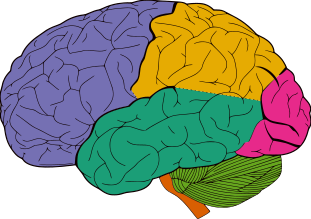
\includegraphics[height=3cm]{dev/wiki/brain_lobes.png}\url{https://en.wikipedia.org/wiki/Frontal_lobe}}
\hspace*{\fill}
\subcaptionbox{\label{fig:nerveFiber}}[.45\textwidth]{
\includegraphics[height=3cm]{dev/wiki/brain_fiber_paths.png}\url{https://en.wikipedia.org/wiki/Association_fiber}}
\hspace*{\fill}
\caption{(a) Illustration of human brain. (b) Illustration of a coronal human brain section. \itodo{a) name brain parts, redo in inkscape}}
\label{fig:human-fiber}
\end{figure}
% 
The frontal, parietal, temporal  and ocipital lobe (see \cref{fig:brainLobes}).
\\
The frontal lobe contains most of the ... functionalities.
The parietal lobe has \dummy{}
The ocipital lobe main function is the signal processing of the visual system.
The temporal lobes contain visual memories as well es auditry functions and language.
\par
The inner part of the brain also include cortival(? -> gm) structures like \dummy{}.
All this structures in the cerebellum and the cerebum contain on thir surfaces (outer as well as inner) a cortical (?) layer, which is filled with cell bodies.
This cells purpase are to process the information of all the signals comming from outside (and inside) the brain.
There are many types of cells involed in this process.
For example some can strengthen a signal or inhibite it.
In the human brain there are several (Billion?) cells which have a high interconnectivity in the local area as well as through the brain to different ...
This high coplex structure is the source of human intelligence, consisnes and much more.
Therefore it is a common goal of humanity to understand the human brain to improve medical treatment as well as \dummy{}.
% 
% \paragraph{Further information}
% This is only a short introduction into the brain architecture.
% It can be further seperated into much more objective parts as well as ...
% This is for example done via cell types and density research like the investigation of cortical layers.
% 
% 
% 
\section{Fiber Architecture} \label{sec:fiberArchitecture}
% 
\begin{figure}[!t]
\centering
\hspace*{\fill}
\tikzset{external/export next=false}
\subcaptionbox{\label{fig:coronalStained}BB 4201: Gray, White Matter, Coronal Section, Stained}[0.6\textwidth]{
\begin{tikzpicture}[]
    \node[inner sep=0pt, anchor = south west] (fig) at (0,0)
    {\includegraphics[width=0.6\textwidth]{dev/brain/BB_4201.png}};
    % \draw[] (0,0) grid (8,5);
    \draw[RED, ultra thick, <-] (5,4) -- ++ (-42:0.75) node[pos=1, anchor=north] {\textbf{WM}};
    \draw[GREEN, ultra thick, <-] (2.4,5) -- ++ (-65:0.75) node[pos=1, anchor=north] {\textbf{GM}};
\end{tikzpicture}
}
\hspace*{\fill}
\subcaptionbox{Cortical layers}[0.3\textwidth]{
\includegraphics[width=0.3\textwidth]{dev/wiki/layers.png}
}
\hspace*{\fill}
% 
\caption[GM, WM, layers]{}
\label{fig:BBrain}
\end{figure}
% 
% 
% 
\begin{figure}[!t]
\centering
% \subcaptionbox{\label{fig:headAndBrain}}[.28\textwidth]{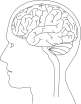
\includegraphics[height=3cm]{gfx/neuroanatomy/human-brain-profile.pdf}}
% \subcaptionbox{}[.42\textwidth]{\includegraphics[height=4cm]{gfx/neuroanatomy/human-brain-section.pdf}}\hfill
% \subcaptionbox{\label{fig:nerveFiber}}[.42\textwidth]{
\includegraphics[angle=90,width=0.75\textwidth,]{gfx/neuroanatomy/neuron-axon_.pdf}
% }
\caption{%(a) Illustration of human brain. 
% (a) Illustration of a coronal human brain section. (b)
Illustration of a neuron with axon and oligodendrocytes. The olegodendrocyte build up a layered lipid structure up, surrounding the axon. The myelin layers are separated along the axon by nodes of Ranvier. \itodo{name parts, ending of axon}}
\label{fig:human-brain}
\end{figure}
% 
Nerve cells are connected via different types of (nerve?) fibers.
A typical nerve cell (see \cref{fig:human-brain}) (if there is such a thing) has a cell body, which processes the incoming information.
The information arrives via dendrites, which are star like tree branches, which will connect to an incoming axon.
The axon is the main (and only) output of the cell.
It travels through the brain to its destination and connects there to a (maybe more or less random) brain cell.
This randomness is also part of the learning process in the brain.
After the brain axons are developed, no new axons are build anymore.
Only the strength of the signals and local structures changes as well as no used connections can be \say{deleted}.
Density of axons \dummy{}.
% Since there are (Billion?) of nerve cells, and there axons need to reach a specific target in a closed volume, the density of nerve fibers is quite high.
There diameter is around $\SI{0.5}{\micro\meter}$ up to several $\si{\micro\meter}$ (see \cref{tag:axonDiameter}).
The axon is surrounded by a myelin sheet, which is a lipid layered structure, build from near by olegodendrides.
These surroundings electric isolates the axon.
This improves the travelling speed of the electric action potential along the axon as well as its signal strength (voltage).
There are many different types of axons.
Some contain a very thick layer of myelin while others have none.
The high density of axons and myelin lets the brain where axons are located, white looking.
Therefore this structure of the brain gets its name \ac{WM}.
The outer cell bodies layer are called \ac{GM}.
In a nissle stained image, where the nerve cells are absorbing light, this is even more visible (see \cref{fig:coronalStained}).
\par
% 
% \begin{figure}[!t]
% 	\centering
% 	\includegraphics{gfx/neuroanatomy/human_wm_after_klinger_dissection.png}
% 	\caption{Electron microscopy image after klinger dissection \cite{destrieux:hal-01261930}. Fiber bundle structures are visible, following the same direction}
% % 	\label{fig:brain_sectioning}
% \end{figure}
% 
\begin{figure}[!t]
	\centering
	\subcaptionbox{}[.49\textwidth]{
	    \includegraphics[width=0.45\textwidth]{dev/brain/auto_seg_axon_0.png}}\hfill
    \subcaptionbox{}[.49\textwidth]{
        \includegraphics[width=0.45\textwidth]{dev/brain/auto_seg_axon_1.png}}
	\caption{Automatic segmentet nerve fiber tissue from an electron microscopy \cite{Abdollahzadeh2019}. }
% 	\label{fig:brain_sectioning}
\end{figure}
% 
Since this \ac{WM} has such a high density of fibers (up to billion in the corpus calosum) it is even under a microscope nearly impossible to investigate single fiber tracts through the brain.
One approach is a myelin staining (see \cref{fig:brainMyelinStain}).
Here nerve fibers which are myelinated are absorbing light (contrast).
Individual nerve fibers can be tracked inside the section.
However already for "smaller" nerve fiber bundles individual nerve fibers are lost.
Especially for dense white matter, no more information can be obtained.
It has also the disadvantage that no 3d orientation information can be easily mapped.
\Cref{fig:brainMyelinStain} shows a section with this technique inside the human thalamus.
It shows different kind of organisations of the nerve fibers.
Nerve fiber bundles are visible (orange) as well as net structures inside the \ac{GM}.
Latter are present to connect the nerve cells with each other inside the \ac{GM}, while the nerve fiber bundles let the axons reach there target area.
\par
% 
\todo{klinger section}
% 
\begin{figure}[!t]
	\centering
	\includegraphics{gfx/neuroanatomy/magic.png}
	\caption{Magic. TPFM auto fluorescence nerve fibers. Origin: \cite{Costantini2020}.}
	\label{fig:brainTPFM}
\end{figure}
% 
\begin{figure}[!t]
	\centering
	\tikzset{external/export next=false}
	\begin{tikzpicture}[]   
     \node[inner sep=0pt, anchor = south west] (fig) at (0,0)
       {\includegraphics[width=\textwidth]{gfx/neuroanatomy/NeuralNet-BrainAtlasDotOrg.png}};
     \draw[Orange, ultra thick] (7.65,6.15) ellipse (1 and 0.5);
     \draw[ProcessBlue, ultra thick] (10,4.5) ellipse (2 and 1);
     \draw[white, ultra thick] (0.5,0.5) -- ++ (0:1) node[pos=0.5, above] {\small $\SI{0}{\micro\meter}$};
    \end{tikzpicture}
% 	\includegraphics[width=\textwidth]{gfx/neuroanatomy/NeuralNet-BrainAtlasDotOrg.png}
	\caption{Myelin Staining. human thalamus, sagital section. \textcolor{Orange}{nerve fiber bundles}. \textcolor{ProcessBlue}{neural net}}
	\label{fig:brainMyelinStain}
\end{figure}
% 
Another tequnique is \ac{TPFM}. 
\cref{fig:brainTPFM} shows a measurement after \ac{3D-PLI} with the \ac{MAGIC} protocol.
This allows fluorescence measurments of the myelin which appears in \ac{3D-PLI} sections after PBS washing \cite{Costantini2021}.
The figure shows the 3d structure of (species, region).
In the lower left part of the volume \ac{WM} is present. 
The border between \ac{WM} and \ac{GM} is in the upper left to the lower right image.
In the upper right corner \ac{GM} is present with individual nerve fibers as well as nerve fiber bundles.
\par
% 
These exemplary data indicate the extreme complexity.
There are a lot more data available.
One comon teqchnique are electorn microscope data.
However the necesarry of a vacuum let the nerve fibers dry out and deform their structure significantly.
\par
% 
For different species with smaller brains, like rodents, imaging techniques like \textit{clearing} have a high potential and could already been used to map an (entire?) brain with axons.
However for a more complex and larger brain, this is up to this point not achieved.
Polarized light imaging, which uses the birefringence property of myelin, is a promising technique, already developed around the 1900, which allows to map the orientation of axons in a brain section.
This technique has, as all microscopic techniques which are using sections, the disadvantage, that the brain has to be cut and measured afterwards.
There are alternative methods like (OCT? \cite{Aumann2019}), which measures the brain section first, and then cuts the upper layer away, and measures the next section afterwards. It uses the reflection of the light than rather the transmitted light through the tissue.
However up to this point no entire large brain like a human brain was measured in its entirety.
Since \ac{3D-PLI} uses the already known sectioning techniques, which are developed since several decades, it can use this knowledge to its advantage.
% 
%
\section{Sectioning}
%
\begin{figure}[!t]
	\centering
    \setlength{\tikzwidth}{0.75\textwidth}
	\inputtikz{gfx/neuroanatomy/brain_sectioning}
	\caption{Illustration of sectioning. a)-b) block with imbedded brain, c) vibrating knife.}
	\label{fig:brain_sectioning}
\end{figure}
% 
For the cutting process, the tissue, \ie{} the brain, has to be frozen and imbedded into a solid material.
One commen material is parafine, however this is not possible for \ac{3D-PLI} \dummy[why?]{}.
For \ac{3D-PLI} it very is important, that the tissue does not build up crystal structures, because these are also birefringence.
Therefore the tissue is first ... into a ... liquid ...
After a time of a few months the tissue will then be frozen into a \SI{-70}{\degree}.
Then the frozen tissue can be fixated with a liquid glue on a cutting plate.
The glue is ...
It is also be used to build up a sourounding fixating material to stabilize the brain in the cutting process.
Additionally markers are fixed which help in the later registration process, which will align the tissue sections in a 3d volume again \cite{Schober2016,Ali2018,Schmitz2018}.
\par
The cutting is done in a microtome (see \cref{fig:brain_sectioning}).
In there the temperature can be held at about \SI{-70}{\degree} and allows no heating of the tissue.
The brain is moved against a vibrating very sharp knife.
This allows for the thin sectioning of about \SI{60}{\micro\meter}.
After the cutting, the tissue is put onto a glass specimen.
Since the tissue is such thin and filigran, it is not always possible to avoid cracks for example.
This also will be as best as possible corrected in the registration process.
The tissue will be ... with a glycerin ... and finally siled with another glass.
To prevent the formation of waves in the tissue, the glass is weighted.
The tissue sections are then stored into a refrigerator at \SI{-70}{\degree\celsius}.
The tissue can then finally be measured in the \ac{3D-PLI} microscopes (see \cref{sec:expSetup} for further techniqule informations).
% 
% 
\section{Axon Literature}
\label{microscopy}
% 
Axon diameter \cite{Liewald2014}:
% 
\begin{table}[!b]
\centering
\pgfplotstabletypeset[
thesisTableStyle,
font=\footnotesize,
col sep=comma,
columns/Name/.style={string type},
columns/Mean/.style={fixed zerofill},
columns/SD/.style={fixed zerofill},
columns/Median/.style={fixed zerofill},
columns/Max/.style={fixed zerofill},
columns/Min/.style={fixed zerofill},
columns/n/.style={dec sep align},
rowbf={1},rowbf={8},rowbf={19},
rowem={2},rowem={5},
rowem={9},rowem={12},rowem={15},
rowem={20},rowem={23},rowem={26},
]{data/axon_distribution.csv}
\caption{axon diameter distribution of the human brain in \si{\micro\meter} \cite{Liewald2014}}
\label{tag:axonDiameter}
\end{table}
% 
\begin{table}[!b]
\centering
\pgfplotstabletypeset[
thesisTableStyle,
font=\footnotesize,
col sep=semicolon,
columns={article,cite,gratio},
columns/article/.style={string type, column name=name, column type = {l}},
columns/cite/.style={string type, column name=cite, column type = {l}},
columns/gratio/.style={string type, column name=$g_{\mathit{ratio}}$},
]{data/gratio.csv}
\caption{human $g_{\mathit{ratio}}$ from invivo mri studies.}
\label{tab:gratio}
\end{table}
% 
axon = 0.5-1.0 diameter (most frequent
thickness of myelin mean = 0.09, median 0.08
-> g-ratio 0.9 (electron microscop, upper boundry)
% 
g-ratio
\cite{Cercignani2017} -> 0.65-0.8 mrt, healty male and female different age, different regions\\
\cite{FitzGibbon2013} -> 0.58-0.84 (Retina), electron microscopy
% 
\itodo{brechungsindex}
% 
% \begin{figure}[!t]
% 	\centering
% 	 \includegraphics[clip, trim=0.65cm 6.25cm 0.4cm 0.5cm]{gfx/neuroanatomy/nature_3d_em_optical_nerve.png}
% 	\caption{\dummy{only show a} Three dimensional electron microscopy reveals changing axonal and myelin morphology along normal and partially injured (*, light green) optic nerves. Origin: \cite{Giacci2018} (reative Commons Attribution 4.0 International License).}
% % 	\label{fig:brain_sectioning}
% \end{figure}
%
%
\cleardoublepage
\setcounter{chapter}{2}
\chapter{Theory}
\label{sec:theory}
% 
\cleanchapterquote{The first principle is that you must not fool yourself and you are the easiest person to fool.}{Richard P. Feynman}{}%\newline
%
\section{Introduction}
The following section lists the physical theories needed to describe the mathematics behind \ac{3D-PLI}. This includes the basic properties of light with the description of their polarization state, the optical models of the tissue, i.e. the nerve fibers and the mathematical description of the experimental setup of \ac{3D-PLI}. The first part of this chapter was written with the help of \cite{demtroeder2, Fliebach2012}.
% 
% 
% 
\section{Electromagnetic Wave}
% 
Light is an electromagnetic wave. Electromagnetism is first fully described by James Clerk Maxwell. He formulated the Maxwell-Equations \cref{eq::maxwell_general}, generalized from the previous work of Johann Carl Friedrich Gau{\ss}, Michael Faraday and Andr\'{e}-Marie Amp\`{e}re and others. 
% 
% \begin{align} 
% \begin{split} \label{eq::maxwell_macro}
%     \nabla \cdot \vec{D} &= 4\pi\rho_\text{f}\\
%     \nabla \cdot \vec{B} &= 0\\
%     \nabla \times \vec{E} &= -\frac{1}{c} \frac{\partial \vec{B}} {\partial t}\\
%     \nabla \times \vec{H} &= \frac{1}{c} \left(4\pi\vec{J}_\text{f} + \frac{\partial \vec{D}} {\partial t} \right)
% \end{split}
% \end{align}
% 
\begin{align} 
\begin{split} \label{eq::maxwell_general}
    \nabla \cdot \vec{E} &= \frac {\rho} {\varepsilon_0}\\
    \nabla \cdot \vec{B} &= 0\\
    \nabla \times \vec{E} &= -\frac{\partial \vec{B}} {\partial t}\\
    \nabla \times \vec{B} &= \mu_0\left(\vec{j} + \varepsilon_0 \frac{\partial \vec{E}} {\partial t} \right)
\end{split}
\end{align}
% 
with $\nabla \coloneqq \left({\frac{\partial}{\partial x}}, {\frac{\partial}{\partial y}}, {\frac{\partial}{\partial z}} \right)$ as vector differential operator, $\vec{E}$ as eletric field, $\rho$ as electric charge density, $\varepsilon_0$ as permittivity of free space, $\vec{B}$ as magnetic field, $\mu_0$ as permeability of free space and $\vec{j}$ as electric current density.
% 
The first equation states no electric field can be generated without an electric charge (charge conservation).
The second equation states, magnetic monopoles does not exists. The basic entity of an magnetic field is a dipole.
The third and forth equation show the interconnection of the electric and magnetic fields in space and time. A change in the electric field yields to a magnetic field and vice versa. Equation forth additional indicates the creation of a magnetic field from a electric current. The maxwell equation fullfill the continoiut ... $\divergence j + \frac{\partial \rho}{\partial t} = 0$
% 
In a vacuum this simplifies with $\rho = 0$ and $\vec{J} = \vec{0}$ to:
% 
\begin{align}
\begin{split} \label{eq::maxwell_vacuum}
  \nabla \cdot \vec{E} &= 0 \quad\\
  \nabla \cdot \vec{B} &= 0 \quad\\
  \nabla \times \vec{E} &= -\frac{\partial\vec B}{\partial t}\\
  \nabla \times \vec{B} &= \mu_0\varepsilon_0 \frac{\partial\vec E}{\partial t}
  \end{split}
\end{align}
% 
With 
\begin{align}
\begin{split} 
    \nabla \times \nabla \times \vec{E} = -\nabla \times \frac{\partial \vec{B}} {\partial t} &= -\frac{\partial} {\partial t} \left( \nabla \times  \vec{B} \right)\\
    &= -\varepsilon_0 \cdot \mu_0 \frac{\partial^2 \vec{E}}{\partial t^2}
\end{split}
\end{align}
% 
the identity $\nabla \times \left( \nabla \times \vec{A} \right) = \nabla(\nabla \cdot \vec{A}) - \nabla^{2}\vec{A}$ and $\mu_0\varepsilon_0 = \frac{1}{c^2}$, with $c$ as the speed of light\footnote{can be derived from Maxwells equation and Lorentz force in a vacuum}, this further simplifies to:
% 
\begin{align}
\begin{split} \label[pluralequation]{eq::maxwell_wave_equations}
  \frac{1}{c^2} \frac{\partial^2 \vec{E}}{\partial t^2} - \nabla^2 \vec{E} &= 0 \\
  \frac{1}{c^2} \frac{\partial^2 \vec{B}}{\partial t^2} - \nabla^2 \vec{B} &= 0
\end{split}
\end{align}
% 
Another common representation is
% 
\begin{align}
\begin{split} \label{eq::maxwell_wave_equations_box}
  \Box \ \vec{E} &= 0 \\
  \Box \ \vec{B} &= 0
\end{split}
\end{align}
% 
with the help of the d'Alembert operator $\Box \coloneqq \partial^a\partial_a = \nabla^2 - \frac{1}{c^2} \frac{\partial^2}{\partial t^2}$.
% 
This also shows $c^2  \frac{\partial B} {\partial z} = \frac{\partial E}{\partial t} \Rightarrow \vec{E} \cdot \vec{B} = 0$ that the electric and magnetic field components are perpendicular to each other.
% 
\subsection{Solving MW Equ in vacuum}
% 
\Cref{eq::maxwell_wave_equations} have the shape of a wave equation and can therefore as known be solved by
% 
% Using the Maxwell equation in vacuum \ref{eq::maxwell_vacuum}, one can find the most simple solution to the differential equation is a wave:
% 
\begin{align}
\begin{split} \label{eq::dgl_solution}
  \vec{E}( \vec{r}, t ) &= g(\phi( \vec{r}, t )) = g( \omega t - \vec{k} \cdot \vec{r} + \varphi)\\
  \vec{B}( \vec{r}, t ) &= g(\phi( \vec{r}, t )) = g( \omega t - \vec{k} \cdot \vec{r} + \varphi )
\end{split}
\end{align}
% 
where $g$ is any well behaved function and therefore also their superposition.
% 
With the help of
% 
\begin{align}
k = \mathopen| \vec{k} \mathclose| = \frac{\omega}{c} =  \frac{2 \pi}{\lambda}
\end{align}
% 
a planar wave can be descriped by
% 
\begin{align}
\begin{split} \label{eq::plane_wave}
\vec{E}(\vec{r}) &= \vec{E}_0 \cdot e^{ -i \, \vec{k} \cdot \vec{r} }\\
 \vec{B}(\vec{r}) &= \vec{B}_0 \cdot e^{ -i \, \vec{k} \cdot \vec{r} }
\end{split}
\end{align}
% 
% 
% 
\subsection{Polarization}
% 
\begin{figure}[!t]
\centering
\setlength{\tikzwidth}{\textwidth}
\inputtikz{gfx/pli/polarization_state}
\label{fig:polarization_state}
\caption{Illustration of light polarization state.}
\end{figure}
% 
This shows, that the light wave travels in direction of $\vec{k}$ (no it does not, you have to show, that k is perpendicular to E and B).
Therefore the light has a property called polarization.
Polarization is the direction of the, usually, electric field component.
% 
A superposition of x and y wave with z equal to direction of propagation yield to the general form
\begin{align}
\vec{E}(z,t) &= \begin{pmatrix} E_{0x} \cdot e^{ -i \phi_x } \\ E_{0y} \cdot e^{ -i \phi_y } \\ 0 \end{pmatrix}
e^{ -i (kz - \omega t)}
\end{align}
%
\begin{figure}[!t]
\centering
\tikzset{external/export=false}
{
% \captionsetup[sub]{textfont=normalsize}
\captionsetup[sub]{position=top, skip=-14pt}
\tikzset{>=stealth}
\tikzset{cross/.pic={
\draw[->] (-{sqrt(2)},0) -- ({sqrt(2)},0) node[anchor=north]{\footnotesize $E_x$};
\draw[->] (0,-{sqrt(2)}) -- (0,{sqrt(2)}) node[anchor=east]{\footnotesize $E_y$};
}}
% 
\subcaptionbox{}[.3\textwidth]{
\begin{tikzpicture}
\pic at (0,0) {cross};
\draw[] (0, 2) node () {linear, horizontal};
\draw[thick, arrows={Stealth[scale=1]-Stealth[scale=1]}] (-1, 0) -- (1, 0);
\draw[] (0, -2) node () {$\begin{pmatrix} 1&0 \end{pmatrix}$};
\draw[] (0, -3) node () {$\begin{pmatrix} 1&1&0&0 \end{pmatrix}$};
\end{tikzpicture}
}
\subcaptionbox{}[.3\textwidth]{
\begin{tikzpicture}
\pic at (0,0) {cross};
\draw[] (0, 2) node () {linear, vertical};
\draw[thick, arrows={Stealth[scale=1]-Stealth[scale=1]}] (0, -1) -- (0, 1);
\draw[] (0, -2) node () {$\begin{pmatrix} 0&1 \end{pmatrix}$};
\draw[] (0, -3) node () {$\begin{pmatrix} 1&-1&0&0 \end{pmatrix}$};
\end{tikzpicture}
}
\subcaptionbox{}[.3\textwidth]{
\begin{tikzpicture}
\pic at (0,0) {cross};
\draw[] (0, 2) node () {linear, $\pi/4$};
\draw[thick, arrows={Stealth[scale=1]-Stealth[scale=1]}] (-1, -1) -- (1, 1);
\draw[] (0, -2) node () {$\begin{pmatrix} 1&1 \end{pmatrix}$};
\draw[] (0, -3) node () {$\begin{pmatrix} 1&0&1&0 \end{pmatrix}$};
\end{tikzpicture}
}
\\[2em]
\subcaptionbox{}[.3\textwidth]{
\begin{tikzpicture}
\pic at (0,0) {cross};
\draw[] (0, 2) node () {left circular};
\draw[thick] plot[domain=0:360,samples=90,smooth] ({cos(\x)},{sin(\x)});
\draw[thick, arrows={-Stealth[scale=1]}] plot[domain=44:45,samples=1] ({cos(\x)},{sin(\x)});
\draw[thick, arrows={-Stealth[scale=1]}] plot[domain=224:225,samples=1] ({cos(\x)},{sin(\x)});
\draw[] (0, -2) node () {$\begin{pmatrix} 1&i \end{pmatrix}$};
\draw[] (0, -3) node () {$\begin{pmatrix} 1&0&0&-1 \end{pmatrix}$};
\end{tikzpicture}
}
\subcaptionbox{}[.3\textwidth]{
\begin{tikzpicture}
\pic at (0,0) {cross};
\draw[] (0, 2) node () {right circular};
\draw[thick] plot[domain=0:360,samples=90,smooth] ({cos(\x)},{sin(\x)});
\draw[thick, arrows={-Stealth[scale=1]}] plot[domain=46:45,samples=1] ({cos(\x)},{sin(\x)});
\draw[thick, arrows={-Stealth[scale=1]}] plot[domain=226:225,samples=1] ({cos(\x)},{sin(\x)});
\draw[] (0, -2) node () {$\begin{pmatrix} 1&-i \end{pmatrix}$};
\draw[] (0, -3) node () {$\begin{pmatrix} 1&0&0&1 \end{pmatrix}$};
\end{tikzpicture}
}
\subcaptionbox{}[.3\textwidth]{
\begin{tikzpicture}
\pic at (0,0) {cross};
\draw[] (0, 2) node () {unpolarized};
\draw[] (0, -3) node () {$\begin{pmatrix} 1&0&0&0 \end{pmatrix}$};
\end{tikzpicture}
}
}
\caption{polarization states, check vector length,\itodo{test speed}} 
\label{fig:polarization_state_vectors}
\end{figure}
%
\Cref{fig:polarization_state_vectors} shows another representation of the polarization sate of a light wave.
It show the component perpendicular to the travelling direction.
Therefore the time variation can be shown on the xy-plane.
Additionally the states can be describe by the Jones or Stokes calculus, later described in \cref{sec:jones,,sec:mueller_stokes}.
% 
% 
% 
\subsection{Light in medium}
% 
The maxwell equations in ... are described above. They can be solved analog to ... . This yields to some special behavier, \eg{} the magnetic and electic field component get out of phase.
However here only the two properties of absorptiona and difraction are described.
They derivation can be found \eg{} \cite{demtroeder2, Fliebach2012}.
% 
\subsection{Absorption}
% 
\begin{align}
    I = I_0 \exp(-\mu x)
\end{align}
% 
Beersche law of absorption with $\mu = \frac{4\pi \kappa}{\lambda_0}$ where $\kappa$ is the imaginary part of the complex refractive index.
% 
\subsection{Refraction}
% 
\begin{figure}[!t]
\centering
\setlength{\tikzwidth}{\textwidth}
\inputtikz{gfx/pli/refraction}
\label{fig:optic_refraction}
\caption{Illustration of refraction.}
\end{figure}
% 
Refraction is the property of light to change direction as it passes from one medium to another. This can be shown by using the full Maxwell equations  for non-conductive material, \ie{} $\vec{j} = 0, \rho = 0$, that the dgl consit out of a primary wave with from atomic medim induced secundary waves, which leads to a reduction of the velocity of the resulting wave. Mathematically this can be described by a complex number $n = c' / c$.
Using this relationship at a boundary surface between two media, one can show that the incident light beam splits into a reflecting and transmittang light wave. The reflecting light wave has the same angle as the incident light beam relativ the the surface normal. The transmitting light beam however due to the reduction of the velocity, changes its direction described by the snellius ...
\begin{align}
    n_0 \sin \alpha = n_1 \sin \beta
\end{align}

% 
\begin{align}
\underline{n} = n + i\kappa
\end{align}
% 
\begin{align}
\begin{split}
\vec{E}(z, t) &= \operatorname{Re}\! \left[\vec{E}_0 \cdot e^{i\, (kz - \omega t)}\right] \\
&= \operatorname{Re}\! \left[\vec{E}_0 \cdot e^{i\, (2\pi(n + i\kappa)z/\lambda_0 - \omega t)}\right] \\
&= e^{-2\pi \kappa z/\lambda_0} \operatorname{Re}\! \left[\vec{E}_0 \cdot e^{i\, (kz - \omega t)}\right]
\end{split}
\end{align}
% 
% 
% 
\subsection{Birefingence}
%
\begin{figure}[!t]
\centering
\setlength{\tikzwidth}{\textwidth}
\inputtikz{gfx/pli/retardation}
\caption{Illustration of retardation.}
\label{fig:optic_retardation}
\end{figure}
% 
\begin{figure}[!t]
\centering
\subcaptionbox{}[.49\textwidth]{
\setlength{\tikzwidth}{0.49\textwidth}
\inputtikz{gfx/pli/ellipsoid_a}}
\subcaptionbox{}[.49\textwidth]{
\setlength{\tikzwidth}{0.49\textwidth}
\inputtikz{gfx/pli/ellipsoid_b}}
\caption{birefringence elipsoid}
\label{fig:index_elipsoid}
\end{figure}
% 
Material can have a different refractive index depending on the relative orientation and polarization of the light beam.
This property is known as birefringence.
The refractive index can be described as the refractive index $n_o$ and extraordinary  $n_e$.
Since these two are perpendicular to each other, one can split the light beam into the same perpendicular parts and describe each by its own.
These two light beams, except for the trivial case of a light beam is perpendicular to the surfave, have a different direction.
However for small relative length (hängt von n ab, bzw der phasenänderung) the two light beams leave the material at the same point and recombined at the end.
The change of phase is called birefringence and is described by the difference between the .. and ...
% 
\begin{align}
    \Delta n = n_e - n_o \> .
\end{align}
% 
This .. can be visualized by the index ellipsoid \cref{fig:index_elipsoid}.
The change of the amplitude and phase can be described by the following techniques.
% 
% 
% 
\subsection{Jones}
\label{sec:jones}
% 
The Jones calculus, introduced by Robert Clark Jones in 1941, describes the polarization state of a light beam by a complex vector $J$:
% 
\begin{align}
    \vec{J} = \begin{pmatrix} E_x \exp(i \phi_x) \\ E_y \exp(i \phi_y) \end{pmatrix}
\end{align}
% 
The amplitude of the perpendicular components are $E_x$ and $E_y$ with their phase $\phi_x$ and $\phi_y$.
Optical elements, which changes the polarization state, such as a polarization filter and retarder, can be desribed by a matrix:
% 
\begin{align}
\begin{split}
\mat{P}_x = 
\begin{pmatrix}
1 & 0 \\ 0 & 0
\end{pmatrix}
, \,
\mat{P}_y = 
\begin{pmatrix}
0 & 0 \\ 0 & 1
\end{pmatrix}
, \,
\mat{M} =
\begin{pmatrix}
e^{i \varphi_x} & 0 \\ 0 & e^{i \varphi_y}
\end{pmatrix}
, \,
\Lambda_{1/4}=
e^{\frac{i \pi}{4}}
\begin{pmatrix}
1 & 0 \\ 0 & -i
\end{pmatrix}
\end{split}
\end{align}
% 
A rotation of the axis can be achieved by a 2d rotation matrix $\mat{R}$:
% 
\begin{align}
\begin{split}
\mat{M}(\theta )=\mat{R}(\theta )\cdot\mat{M}\cdot\mat{R}(-\theta )
, \>
\mat{R}(\theta ) = 
\begin{pmatrix}
\cos \theta & -\sin \theta \\
\sin \theta & \cos \theta
\end{pmatrix}
\end{split}
\end{align}
% 
% 
% 
\subsection{M\"uller-Stokes}\label{sec:Mueller-Stokes}
\label{sec:mueller_stokes}
% 
Analog to \cref{sec:jones} the M\"uller-Stokes formalism, described by George Gabriel Stokes in 1852, also describes the polarication state of a light beam.
However it does not use the absolute .. but the relative polarication between both components:
% 
\paragraph{Stokes vector}
\begin{align}
\begin{split}
S_0 &= I \\
S_1 &= I p \cos 2\psi \cos 2\chi \\
S_2 &= I p \sin 2\psi \cos 2\chi \\
S_3 &= I p \sin 2\chi
\end{split} \hspace{-6em}
\begin{split}
& \equiv \langle E_x^{2} \rangle + \langle E_y^{2} \rangle \\
%  & = \langle E_a^{2} \rangle + \langle E_b^{2} \rangle \\
%  & =  \langle E_l^{2} \rangle + \langle E_r^{2} \rangle \\
& \equiv \langle E_x^{2} \rangle - \langle E_y^{2} \rangle \\
& \equiv \langle E_a^{2} \rangle - \langle E_b^{2} \rangle \\
& \equiv  \langle E_l^{2} \rangle - \langle E_r^{2} \rangle
\end{split}
, \,
\vec{S} =
\begin{pmatrix} S_0 \\ S_1 \\ S_2 \\ S_3\end{pmatrix}
\end{align}
% 
% \begin{align}
% \begin{split}
% S_0 & \equiv \langle E_x^{2} \rangle + \langle E_y^{2} \rangle \\
%  & = \langle E_a^{2} \rangle + \langle E_b^{2} \rangle \\
%  & =  \langle E_l^{2} \rangle + \langle E_r^{2} \rangle \\
% S_1 & \equiv \langle E_x^{2} \rangle - \langle E_y^{2} \rangle \\
% S_2 & \equiv \langle E_a^{2} \rangle - \langle E_b^{2} \rangle \\
% S_3 & \equiv  \langle E_l^{2} \rangle - \langle E_r^{2} \rangle
% \end{split}
% \end{align}
% 
Therefore the phase can not be described anymore.
However the relative phase information is stored and can be used to describe also polarization states of polarization filters, which can not be described by Jones.
Aanlog to Jones one can formulate the matrices for the optical components:
% 
\paragraph{Linear Polarizer}
\begin{align}
\mat{P}_x=\frac{1}{2}
\begin{pmatrix}
    1 & 1 & 0 & 0 \\
    1 & 1 & 0 & 0 \\
    0 & 0 & 0 & 0 \\
    0 & 0 & 0 & 0
  \end{pmatrix}
, \,
\mat{P}_y=\frac{1}{2}
\begin{pmatrix}
     1 & -1 & 0 & 0 \\
    -1 &  1 & 0 & 0 \\
     0 &  0 & 0 & 0 \\
     0 &  0 & 0 & 0
\end{pmatrix}
\end{align}
% 
\paragraph{retarder}
\begin{align}
\mat{M}=\
\begin{pmatrix}
    1 & 0 & 0 &  0 \\
    0 & 1 & 0 &  0 \\
    0 & 0 & \cos \delta & \sin \delta \\
    0 & 0 & -\sin \delta &  \cos \delta
\end{pmatrix}
\end{align}
% 
\paragraph{Quarter-wave plate (fast-axis vertical)}
\begin{align}
\Lambda_{1/4}=\
\begin{pmatrix}
    1 & 0 & 0 &  0 \\
    0 & 1 & 0 &  0 \\
    0 & 0 & 0 & -1 \\
    0 & 0 & 1 &  0
\end{pmatrix}
\end{align}
% 
\paragraph{Rotation Matrix}
\begin{align}
\mat{R}(\theta)=
\begin{split}
\begin{pmatrix}
    1 &                0 &               0 & 0 \\
    0 & \cos{(2\theta)} & -\sin{(2\theta)} & 0 \\
    0 & \sin{(2\theta)} & \cos{(2\theta)} & 0 \\
    0 &                0 &               0 & 1
  \end{pmatrix}
\end{split}
\end{align}
% 
% \paragraph{Rotation Matrix}
% \begin{align}
% \frac{1}{2}
% \begin{pmatrix}
%     1 &                0 &               0 & 0 \\
%     0 &  \cos{(2\theta)} & \sin{(2\theta)} & 0 \\
%     0 & -\sin{(2\theta)} & \cos{(2\theta)} & 0 \\
%     0 &                0 &               0 & 1
% \end{pmatrix}
% \end{align}
\todo{matrix multi}
% 
% \section{Tissue Discretization}
% % 
% By deviding the volume into small diskreticed subvolumes, one can multiply the .. all together and ... (analog Riemann sum)
% \begin{align}
%     \int F \, dt \approx \sum_n F \, \Delta t
% \end{align}
% see simulation?
% 
%  see simulation
% \paragraph{Micro vs Macro:}
% % 
% % \begin{align}
% %   \int_{y_\textit{min}}^{y_\textit{max}} \vec{v}(y) \,dy\\
% %   x = const
% %   y = y(\alpha,x) = tan(\alpha) \cdot x\\
% %   \vec{v}_r = \begin{pmatrix} \cos(\alpha)\\ \sin(\alpha)\\0\end{pmatrix}, \, \vec{v}_p = \begin{pmatrix} 0\\ 0\\1\end{pmatrix}\\
% %   \vec{v}_r = \begin{pmatrix} \cos(\arctan(y/x))\\ \sin(\arctan(y/x))\\0\end{pmatrix}\\
% %   \int_{y_\textit{min}}^{y_\textit{max}} \vec{v}_p(y) \,dy = (y_\textit{max} - y_\textit{min}) \cdot e_z\\
% %   \int_{y_\textit{min}}^{y_\textit{max}} \vec{v}_r(y) \,dy = \int_{y_\textit{min}}^{y_\textit{max}} \cos(\arctan(y/x)) dy \cdot e_x \\
% %   = x\left(\sinh^{-1}(y_\textit{max}/x) - \sinh^{-1}(y_\textit{min}/x)\right) \\
% %   = 2x \left(\sinh^{-1}\left(\frac{2\sqrt{R-x^2}}{x}\right)\right)
% % \end{align}
% % 
% % \begin{align}
% %     % \frac{\oint \vec{v}_z \mathrm{d}A}{\oint \vec{v}_x \mathrm{d}A} = 
% %     % \frac{\int_{-1}^{1}\abs{\vec{v}} \mathrm{d}x}{\int_{-\frac{\pi}{2}}^{\frac{\pi}{2}} \abs{\vec{v}} \cos(\varphi) \mathrm{d}\varphi} =
% %     % \frac{2}{1}
% %     \frac{A_{\Box}}{A_{\circ}} = \frac{4}{\pi}
% % \end{align}
% % 
% \todo{why 2*dn?}
% 
\section{Experimental Setup}\label{sec:expSetup}
%
\begin{figure}[!t]
    \captionsetup[sub]{position=top}
    \setlength{\tikzwidth}{\textwidth}
	\centering
	\subcaptionbox{\label{setup-lap} \ac{LAP}}[\textwidth]{
% 		\resizebox{0.95\textwidth}{!}{
		\inputtikz{gfx/pli/pli_setup}
% 	}
	}\\
	\subcaptionbox{\label{setup-pm} \ac{PM}}[\textwidth]{
% 		\resizebox{0.95\textwidth}{!}{
		\inputtikz{gfx/pli/pli_setup_pm}
% 	}
	}
	\caption{Illustration of PLI setup.}
	\label{fig:pli_setup}
\end{figure}
%
\begin{figure}[!t]
    % \captionsetup[sub]{position=top}
    \setlength{\tikzwidth}{0.3\textwidth}
	\centering
	\subcaptionbox{\ac{LAP}}[.49\textwidth]{
			\inputtikz{gfx/pli/pli_detail}}\hfill
	\subcaptionbox{\ac{PM}}[.49\textwidth]{
			\inputtikz{gfx/pli/pli_detail_pm}}
	\caption{Illustration of detail PLI setup.}
	\label{fig:pli_detail}
\end{figure}
%
The \ac{3D-PLI} setup is described in \cite{Axer2011} with the tiltable light beam microscope (LMP) in \cite{Wiese:887678}.
For the routine measurements two (three) microscope systems are currently in use.
The first use of a high throughput microscope is the \ac{LAP} with a pixel size of about \SI{60}{\micro\meter}. \footnote{can be change by the optic also to $\SI{40}{\micro\meter}$ and $\SI{20}{\micro\meter}$, but remains for the routine measurements with $\SI{60}{\micro\meter}$.}
It consist out of a led light source (\SI{525}{\nano\meter}), a rotatable polarization filter, a rotatable quarter wave retarder, the specimen stage, which can be tilted for oblique views, a rotatable polarizer.
Both polarizer and quarter wave retarder are rotated at the same time.
The both polarizers have a phase offset of $\SI{90}{\degree}$, the first polarizer and the quarter wave retarder of $\SI{45}{\degree}$ (see (see \cref{setup-lap}).
The second system \ac{LMP3D} microscope fullfills the same measurments, however the retarder is placed after the tissue specimen and fixed with the polarizer without any rotations (see \cref{setup-pm}).
Mathematically it measures the same signal.
\footnote{The rotatable filters of the \ac{LAP} has the advantage, that noise like dust particles can be easy identified and removed. Since the microscop is in a more confined "box" this is not necesarry.}
A difference is that the optical path is in reverse to the \ac{LAP} system.
Since there is a mirror in the path, the image is flipped again so that the coordinate systems stays the same (see \cref{fig:pli_detail}).
% 
\subsection{Signal}
% 
From the M\"{u}ller Matrices (\cref{sec:Mueller-Stokes}) as shown in \cite{MenzelMaster,MenzelDissertation}, that the intensity signal, measured by the \ac{CCD}-sensor, follows a sinusiodal curve:
% 
% \begin{align}
% I = \underbrace{\frac{I_0}{2}}_{\mathclap{\mathit{transmittance}}}
%     \bigl[ \sin\bigl(2\rho - 2{\underbrace{\vphantom{\frac{I_0}{2}} \varphi}_{\mathclap{\mathit{direction}}}} \bigr)
%     \cdot \sin \bigl( {\underbrace{\vphantom{\frac{I_0}{2}} 2\pi\frac{d \dn}{\lambda} \cos^2\left( \alpha \right)}_{\mathclap{\delta \, \coloneqq \, \mathit{retardation}}}} \bigr) \bigr]
% \end{align}
\begin{align}
\label{eq:pli_signal}
\begin{split}
I =\frac{I_0}{2}\bigl[ \sin\bigl(2\rho - 2\varphi \bigr)\cdot \sin \bigl( 2\pi\frac{d \dn}{\lambda} \cos^2\left( \alpha \right) \bigr) \bigr] \\
\text{with} \enspace \delta \coloneqq 2\pi\frac{d \dn}{\lambda} \cos^2\left( \alpha \right) \enspace 
\text{and} \enspace \trel \coloneqq \frac{d \dn}{\lambda}
\end{split}
\end{align}
% 
Since \cref{eq:pli_signal} describes a sinosoidal signal, the fourier analysis is a obvious choise.
For a discrete, aquidistant measurement of the rotation angles $\rho$, one can use the fourier series with the three coefficients to describe the signal:
% 
% \begin{align}
% \begin{split}
% A \sin(\omega t + \alpha) + B \sin(\omega t + \beta) &= \sqrt{C^2 + D^2} \cdot \sin \, \left( \omega t + \tan^{-1} \left( \frac{D}{C} \right) \right)
% \end{split}
% \\
% \begin{split}
% C &= A \cos(\alpha)+ B \cos(\beta)\\
% D &= A \sin(\alpha)+ B \sin(\beta)
% \end{split} \nonumber 
% \end{align}

\begin{align}
\begin{split}
\rho &= [\SI{0}{\degree}, \frac{1\cdot180}{N+1}\si{\degree}, \frac{2\cdot180}{N+1}\si{\degree}, ..., \frac{N\cdot180}{N+1}\si{\degree}]\\
a_0 &= \frac{1}{N} \sum(\mathit{data})\\
a_1 &= \frac{2}{N} \sum(\mathit{data} \cdot \sin(2 \cdot \rho)\\
b_1 &= \frac{2}{N} \sum(\mathit{data} \cdot \cos(2 \cdot \rho)
\end{split}
\end{align}

With these the final \ac{3D-PLI} modalities are calculated:

\begin{align}
\begin{split}
\mathit{transmittance} &= 2 \cdot a_0\\
\mathit{direction} &= 0.5 \cdot \atantwo(-b_1 / a_1)\\
\mathit{retardation} &= \frac{\sqrt{a_1^2 + b_1^2}}{a_0}
\end{split}
\end{align}



% 
\subsection{Tilted signal}
% 
To be able to analyse the inclination $\alpha$ one has to distiguish the relative strength of the birefringence from the $\cos^2(\alpha)$.
For this purpose a tiltable specimen was developed, which allows measuring the light signal through the tissue with a different angle of incidenc.
This mean, that tissue and therefore the nerve fibers also change their orientation by the tilting angles $\theta, \varphi$.
Additionally the distance the light travels through the tissue, elongigates by $1/\cos(\theta)$ \cref{fig:tilted_side_view}.
% 
Depending on the \pixelsize{}, in the case of the \ac{LAP} system, this light travels though the same volume, but with another orientation.
Therefore a measurement of multiple light paths can be ... and the resulting signals can be used to analyse the inclination and relative birefrigente tissue thickness \trel{}.
In the case of a tiltible specimen, the angle of incidence on the glass ... and the tissue also changes the angle of the light by snellius law.
All angles mentiont here are if not specified always the change of angle of the light inside the tissue (see \cref{fig:tilting_camera_view}). 
This also leads to a perspective shift, which has to be corrected by a registration process.
In this case an affine transformation.
% 
In \cite{Schmitz2018} this analys published under the name of \ac{ROFL}, which builds up on the work of \cite{Wiese:887678}.
The idea is to fit the measured signals of all light paths simultaniously.
Because the change of signal is proportional to the $\cos(\alpha)$ this however means, that for steep fibers, the changes are not only small, but also the amplitude of the signal is very small.
This leads to the problem of increasing uncertanty with increasing inclination angle.
\\
A further problem is that for a smaller \pixelsize{} the light path cannot be neglected anymore.
For the \ac{LMP3D} system this means, that with a maximal tilting angle of about $\SI{3}{\degree}$ and a usually tissue thickness of $\SI{60}{\micro\meter}$ the light path is measured in n pixels away from the non tilting case, if the rotation point is in the center of the tissue.
\\
However for homoginoius tissue, like the \ac{WM} may be some regions, the analysis technique can still be applied.
A change in density, orientation or dispersion however will lead to a false result.
% 
% 
% 
\section{Orientation}
% 
\begin{figure}[!t]
\centering
\setlength{\tikzwidth}{0.4\textwidth}
\begin{center}
\begin{tabular}{m{6cm}m{6cm}}
\includegraphics[width=\tikzwidth]{gfx/pli/color_sphere.png}
&
\inputtikz{gfx/pli/hsv_sphere}
\\
\begin{minipage}[t]{0.42\textwidth}
\leavevmode\subcaption{2d hsv sphere}
\end{minipage}
&
\begin{minipage}[t]{0.42\textwidth}
\leavevmode\subcaption{\label{fig:sphere}3d hsv sphere}
\end{minipage}
\end{tabular}
\end{center}
% 
\vspace{-1em} % because of tabular?
\caption{collor spheres}
\label{fig:spheres}
\end{figure}
% 
% 
The orientation of the birefringence axis is descibed by the direction angle $\varphi$ and inclination angle $\alpha$ (see \cref{fig:sphere}).
To be able to show a 3d information, the \textit{hsv-black} is usually shown in \ac{3D-PLI}.
It color code the orientation by:
\begin{align}
\begin{split}
    H &= \varphi/\pi\\
    S &= 1\\
    V &= 1-\alpha / \pi/2
\end{split}
\end{align}
This way the color corresponds to the direction, and the color value to the inclination.
Since the orientation, unlike a vector, covers only a half sphere, the colors are point symmetric.
% 
% fig:spheres
% 
% 
\section{optical resolution}
\label{sec:opticalResolution}
% 
The optical resolution of an imaging system describes the minimal size of on object which can still be resolved.
This property is limited by aberration and diffraction which both cause a blurring of the resulting image.
Ernst Abbe described as on of the first that the resulition corrlates with the lightwave $\lambda$: 
\begin{align}
d=\frac{ \lambda}{2 n \sin \theta} = \frac{\lambda}{2\mathrm{NA}} \> .
\end{align}
$d$ is the minimal resolvable distance, $n$ the refractive index, $\theta$ the angle of a spot light, which can be combined to the better known numerical aperture $\mathrm{NA}$.
This results in an absolute threshold for a light microscope above which the resolution can no longer be improved.
For the wavelength used in \ac{3D-PLI} with $\lambda = \SI{525}{\nano\meter}$ and a numerical apperatur of $\mathrm{NA} = \SI{}{}$ this yields to a limit of \dummy{}.
% 
\begin{figure}[!t]
\setlength{\tikzwidth}{0.45\textwidth}
\centering
% \subcaptionbox{}{
\inputtikz{gfx/pli/rayleigh}
\caption[Raylay criterium]{rayleigh criteria. The minima of the one function is in the maxima of the other.}
\label{fig:rayleigh}
\end{figure}
% 
%
\cleardoublepage
\part{Software}
% \acbarrier
\parttoc
\setcounter{chapter}{3}
\chapter{Nerve fiber modelling}
\label{chap:sof:modelling}
% 
In \cref{chap:neuro} both the structure of nerve fibers and the macroscopic structure of \ac{WM} were described.
The question is how to represent such a structure in a computer algorithm.
For simple fiber configurations, \eg{} parallel, linear nerve fibers, this may be quite straightforward.
However, it has been shown that irregular, non-symmetric nerve fiber configurations are necessary to obtain a realistic result without diffraction patterns \cite{MenzelDissertation}.
This means that any kind of pattern that may exist should ideally be representable.
\par
%
Many solutions are already available.
A common one comes from visualization.
A rope or fiber, \ie{} a raw object, is defined by a trajectory with a radius.
From this, a surrounding mesh is generated.
In visualization, the mesh is used to apply textures to represent a surface.
The same meshes are used in Monte Carlo simulations \ac{dMRI} \cite{Ginsburger2019,ginsburgerDis2019}, among others.
In this type of simulation, the meshes help calculate whether a water molecule travels through the surface of a nerve fiber, i.e., the surface of the mesh.
However, this representation is very computationally intensive because the number of triangles that must be present in the mesh is quite high for useful accuracy.
\par
%
An even more crucial task is to ensure that the nerve fibers do not overlap.
In simulations where the wave nature of light is modeled, this leads otherwise to incorrect results.
To achieve this, either the user must define such a structure in advance, or a computer algorithm must build such structures from input parameters.
Considering the immense number of configuration possibilities that nerve fibers can have even in a small volume, the task is almost impossible for a user to solve except for trivial configurations.
The same is true for a computer algorithm.
One could write an algorithm that defines a single fiber in a volume and then places the next one, making sure that none overlaps and so on.
This works well up to a point.
Even if an algorithm always finds a solution to find a path through an already filled volume, at some point the volume will appear to be full, but still have plenty of free space between fibers.
Of course, one can minimize this behavior by trying to place nearly parallel fibers, but again, looking at real tissue data, \eg{} \cref{fig:brainTPFM}, this does not reflect reality.
Even in a fiber bundle, the fibers are so densely packed that you can't just add another fiber in a way that wastes volume over time (\ie{} add more fibers).
\par
%
The solution found in this work is to allow the placement of nerve fibers in any way and without any restriction.
However, the overlap must then be removed.
The idea is quite simple.
Check all fibers for collisions with each other.
If a collision occurs, try to remove it by moving the colliding parts slightly away from each other.
Repeat this step until all collisions are removed.
\par
%
This idea \cite{Matuschke2019} with all its necessary prerequisites is described in detail in the following chapter.
First, the representation of a nerve fiber is defined in a way that it already takes into account to be as performant as possible for the collision process.
Then, additional \textit{building} functions are designed to help the user quickly define a volume with nerve fibers.
Finally, the solution algorithm for resolving the collisions with its parallel components is explained in detail.
In addition, another approach based on this idea and developed in this work with colleagues from \ac{dMRI} is explained in detail.
This one focuses on the placement of neurons such as astrocytes or olegodendrocytes with their (arms) in the volume.
The collaboration is obvious since both simulation techniques study the same type of tissue models.
Since these models focus on non-overlapping tubular structures, they can also be applied to other fibrous structures such as skeletal muscle fiber.
\par
%
All described algorithms here are part of the toolbox \ac{fastPLI} \cite{Matuschke2019, Matuschke2021}, which is described in detail in \cref{chap:Software}.
%
%
%
\section{Nerve fiber representation}
\label{sec:nerve_fiber_representation}
%
Nerve fibers themselves are cable-like structures surrounded by an electrically insulating lipid layer of myelin (see \cref{sec:fiberArchitecture}).
Both the diameter of the axon and the thickness of the myelin can vary greatly from fiber to fiber (see \cref{sec:axonMicroscopy}).
This means that the representation of nerve fiber models should be able to represent such variations as well.
\par
%
As described in \cref{sec:fiberArchitecture} \ac{WM} consist of nerve fibers packed tightly together in nerve fiber bundles.
These bundles can join/divide with other bundles and traverse the brain to connect one region to another.
The bundles are able to cross each other, either by crossing the individual nerve fibers or bypassing the fiber bundles in some sort of interwoven structure.
These structures are a key element in the study of \ac{3D-PLI}.
Therefore, it is particularly important that the models are able to form such structures without overlapping individual fibers.
\par
%
One way of representing it is a parametric function describing a path in 3D space, a trajectory.
In addition, a fourth element could describe the radius of the fiber at the same point:
% 
\begin{align}
f(t) \rightarrow (x(t),y(t), z(t), r(t))
\end{align}
% 
However, this representation does not allow simple subsequent changes, such as resolving collisions.
For this purpose, individual elements are more manageable, allowing movement or deformation.
Therefore, the function or fiber is divided into smaller discrete segments.
%
\begin{figure}[!t]
    \setlength{\tikzwidth}{0.85\textwidth}
    \centering
    % \tikzset{external/export next=false}
    \inputtikz{gfx/model/fiber_model}
	\caption[]{Representation of a nerve fiber from a list of spheres.}
	\label{fig:fiberReb}
\end{figure}
%
Therefore, the fiber can be described by a list of 4d points $(x,y,z,r)$, which can be interpreted as a chain of cylindrical fiber segments (see \cref{fig:fiberReb}):
\begin{align}
\begin{split}
\mathit{fiber} = \left\{ \vec{p}_i=(x_i,y_i,z_i), r_i \mid x,y,z \in \mathbb{R}, \, r \in \mathbb{R^+}, \, i \in \{0,1,...,N_{\mathit{points}}-1\}\right\} \\
\mathit{fiber\_segment}_i = (\vec{p}_i, \vec{p}_{i+1}, r_i, r_{i+1}), \, i \in \{0,1,...,N_{\mathit{points}}-2\}
\end{split}
\end{align}
%
\begin{figure}[!t]
    \centering
    \setlength{\tikzwidth}{0.5\textwidth}
    \inputtikz{gfx/model/capsule}
	\caption{schematic \acreset{CC} \ac{CC}}
	\label{fig:conical}
\end{figure}
%
Since the fiber radius can change from one point to an adjacent point, the segment can be conical (see \cref{fig:conical}).
Therefore, the fiber segments describe a \ac{CC}.
\par
%
This representation has the advantage over a mesh representation of a surface that much less data is needed for the representation.
This will increase the computational speed, which will be crucial for a collision solving algorithm.
%
% 
% 
\section{Sandbox}\label{sec:sandbox}
%
In computer game terminology, a \textit{sandbox mode} is a game mode that allows the player to build and design anything at no cost.
Analogous to this feature is the \pymodule{fastpli.model.sandbox}, which allows the user to easily and quickly design standard geometric configurations of nerve fibers and bundles.
Since nerve fibers are usually arranged in bundles, the design methods focus on generating nerve fiber bundles from a 2d pattern (seed points) and a nerve fiber bundle trajectory.
\par
%
This module is divided into two successive submodules.
The first module handles the seeding process, while the second part builds up a nerve fiber bundle or volume filled with individual fibers from seed points.
%
\subsection{Seeding fiber bundles}\label{sec:seeds}
%
\begin{figure}[!t]
    \def\tikzheight{0.25\textwidth}
    \centering
    \subcaptionbox{\label{fig:triGrid}equilateral triangle grid}[.32\textwidth]{
    \inputtikz{gfx/model/triangular_grid}}
    \hfill
    \subcaptionbox{\label{fig:rndGrid}random grid}[.32\textwidth]{
    \inputtikz{gfx/model/rnd_circle_points}}
    \hfill
    \subcaptionbox{\label{fig:crossBundle}populated fiber bundles}[.32\textwidth]{
    \inputtikz{gfx/model/crossing_bundle}}
	\caption{Populating fiber bundles with seed points.}
% 	\label{fig:}
\end{figure}
%
Seed points are stored as a list of 2d points:
\begin{align}
\mathit{seeds} = \left\{ \vec{p}_i=(x_i,y_i) \mid x,y \in \mathbb{R} , \, i \in \{0,1,...,N_{\mathit{seed\_points}}-1\}\right\}
\end{align}
%
To form particularly dense fiber bundles, a method for generating an equilateral triangular grid was implemented (see \ref{fig:triGrid}).
Mathematically, this yields the most densely packed pattern for a 2d circle with equal radius packed area.
However, this very regular symmetric grid can lead to unrealistic results (\eg{} diffraction pattern in Maxwell simulation).
It should therefore only be used as an initial configuration.
Since the initial configurations are often unknown, it is probably best to choose a random distribution (see \cref{fig:rndGrid}).
For a circular boundary, this is done with:
% 
\begin{equation}
\begin{split}
\varphi &= \mathrm{uniform}(0,2 \pi) \\
r &= R \sqrt{\mathrm{uniform}(0,1)}
\end{split}
\quad\Rightarrow\quad
\begin{split}
x = r \cos(\varphi)\\
y = r \sin(\varphi)
\end{split}
\end{equation}
%
%
%
\subsection{Populating fiber bundles}\label{sec:fillBundle}
%
\begin{figure}[!t]
    \centering
    \resizebox{.75\textwidth}{!}{
    \includegraphics{dev/gfx/circle_bundle.png}}
    % }
	\caption{Bending fibers along trajectory $\vec{f}(t) = \left(\cos(t), \sin(t), 0 \right)$ \todo{more interesting example}}
	\label{fig:bendingFiberBundle}
\end{figure}
%
\begin{figure}[!t]
    \centering
    \setlength{\tikzwidth}{0.75\textwidth}
    \inputtikz{gfx/model/min_torsion}
	\caption[]{Left: Plane of seed points. Right: plane are rotated and placed along the path. At the end, the plane has the same normal vector as the starting plane, but due to the principle of minimum rotation, the plane is rotated along the normal vector.}
	\label{fig:torsion}
\end{figure}
%
To populate a fiber bundle, the plane containing the seed points is placed at each fiber bundle point $\vec{fb}_i$ along the trajectory.
Essentially, for each resulting $\mathit{fiber}_j$, this means:
% 
\begin{align}
    \mathit{fiber}_j = \left\{ \mat{R} \cdot (x_j, y_j, 0) + \vec{fb}_i \, | \, i \in \{0,1,...,N_{\mathit{seed\_points}}-1\}\right\}
\end{align}
% 
However, the question is which rotation matrix $\mat{R}$ has to be applied.
Since a trajectory is only a 2d object, \ie{} is a line, so no unique normal vector can be defined in space.
In mathematics, the torsion of a curve can be defined with a principal normal vector and a binormal vector.
However, this has the problem that the line has a torsion for a helical function, meaning that the line rotates along its path.
This would mean that the individual fibers would rotate around the path of the fiber bundle if the seed point plane were placed according to the principal and binormal vectors.
This is possible in principle, but practically non-existent in real tissue.
\par
% 
A more reasonable solution would be to perform a rotation such that the rotation along the fiber bundle trajectory is minimal.
This can be achieved by computing the rotation matrix that would rotate the current tangent vector \textcolor{BLUE}{$\vec{t}(i)$} to that of the nearest point $\vec{t}(i+1)$.
The rotation matrix $\mat{R}(\vec{a}, \vec{b})$ can be calculated, except for $\vec{a} || \vec{b}$ via
\begin{align}
\begin{split}
    \vec{a} =& \; \vec{a} / |\vec{a}|\\
    \vec{b} =& \; \vec{b} / |\vec{b}|\\
    \vec{v} =& \; \vec{a} \times \vec{b}\\
    c =& \; \vec{a} \cdot \vec{b}
\end{split}
\quad
\begin{split}
    \mat{U} =& \begin{pmatrix} 0 & \vec{v}_z & -\vec{v}_y\\ -\vec{v}_z & 0 & \vec{v}_x\\ \vec{v}_y & -\vec{v}_x & 0\end{pmatrix}\\
    \mat{R} =& \; \mathbb{1} + \mat{U} + (\mat{U} \cdot \mat{U}) \cdot (1 - c) / |\vec{v}|^2
\end{split}
\end{align}
% 
This tool enables the following procedure:
First, place the seed point plane at the first fiber bundle point $\vec{fb}_0$ and rotate it by $\mat{R}(\hat{\vec{e}}_z, \vec{t}_0)$.
Then, for each step, the plane is rotated at its original origin according to $\mat{R}(\vec{t}_i, \vec{t}_{i+1})$ and placed on $\vec{fb}_{i+1}$.
To smooth the transition, the tangential vector at step $i$ is calculated as follows.
\begin{align}
    \vec{t} = \frac{1}{2} \frac{\vec{fb}_{i-1} + \vec{fb}_{i+1}}{|\vec{fb}_{i-1} + \vec{fb}_{i+1}|}
\end{align}
%
Finally, all points belonging to a fiber can be stored in a fiber bundle object.
An example is shown in \cref{fig:bendingFiberBundle}.
%
%
%
\subsection{Cube models} \label{sec:cubeModelBuilding}
%
\begin{figure}[!t]
    \centering
    \setlength{\tikzwidth}{0.5\textwidth}
    \inputtikz{gfx/model/cube_build}
	\caption{Populating a cuboid with straight fibers initialized by seed points along the direction $\vec{v}$.}
    \label{fig:cubeBuild}%
\end{figure}
%
As will be shown later, cube-shaped models are very interesting to study, since a pixel in the \ac{3D-PLI} setup is a cube with the height of the tissue thickness.
Therefore, a method exists to fill such a volume with a fiber population of orientation $\vec{v}$ (see \cref{fig:cubeBuild}).
The individual fibers are initialized as usual with a seed point plane.
This plane is virtually placed in front of the cubic volume end behind it in the direction of the orientation, so that the origins of the seed point planes coincide with the origin of the cube.
Then the seed points are virtually connected.
When a line meets the volume, the entry and exit points are calculated and stored as fibers of the fiber bundle.
%
%
%
\subsection{Cylindric models}
%
\begin{figure}[!t]
    \centering
    \setlength{\tikzwidth}{0.31\textwidth}
    \subcaptionbox{\label{fig:cylCircular}%
        Circular population.
    }[.33\textwidth-1ex]{
    \inputtikz{gfx/model/cylinder_circular}}\hfill
    %
    \subcaptionbox{\label{fig:cylRadial}%
        Radial population.
    }[.33\textwidth-1ex]{
    \inputtikz{gfx/model/cylinder_radial}}\hfill
    %
    \subcaptionbox{\label{fig:cylParallel}%
        Parallel population.
    }[.33\textwidth-1ex]{
    \inputtikz{gfx/model/cylinder_parallel}}
	\caption{Colonization of cylindrical objects. The green area shows the area corresponding to the seed points in the xy-plane. The coordinate system \textcolor{RED}{red} indicates the coordinate origin for the seed points.}
\end{figure}
%
The last method allows, among other things, to create circular arcs from fibers.
It uses a cylindrical volume as a template.
Since a cylinder has three symmetries, a radial, an angular and the length, all three have been implemented to provide a way to populate the volume.
\par
%
First, the coordinate system must be defined.
The cylinder with outer radius $r_{\mathit{out}}$ and inner radius $r_{\mathit{in}}$ is aligned along the z-axis with height $h$ and starts at $(0,0,0)$.
In addition, the cylinder can be cut radially at a directional angle $\alpha$ to $\beta$ to fill only a portion of it.
\par
%
The following applies to all methods used: If the seed point plane leaves the cross-section plane to be filled, the seed points lying outside are ignored.
%
\paragraph{a) circular}
mimics a radial path of the cylinder (see \cref{fig:cylCircular}).
The seed points are placed along the surface of the cross section of the first $\alpha$ direction angle.
The origin of the seed point plane is placed on the origin of the cylinder.
From there, the fiber is circular to the second $\beta$ direction angle.
The step size of the circular path can be changed.
%
\paragraph{b) radial}
The fibers are placed from the inner wall to the outer wall of the cylinder.
The seed point plane is therefore placed at the inner wall with the origin at the bottom corner of the first angle $\alpha$ (see \cref{fig:cylRadial}).
The fibers are then generated radially until they meet the outer wall of the cylinder.
Thus, the density of the fibers decreases along their path.
%
\paragraph{c) parallel}
The fibers are aligned along the cylinder (see \cref{fig:cylParallel}).
Here, the seed points are in the lower plane, with the two origins in the same point (see \cref{fig:cylParallel}). The orientation of the plane is aligned with the x-axis at $\SI{0}{\degree}$
%
%
%
\section{Solving fiber collisions}
\label{sec:Solver}
%
The focus of the following algorithm is to allow the user to define any fiber path.
This allows for the greatest possible freedom in initialization.
Of course, since the fibers are 3D volume objects, in most cases there will be overlaps with other fibers.
The aim of the following algorithm is to find and solve such collisions by moving the affected fiber segment in such a way that a collision-free volume is created by minimal displacement.
This allows the user to specify complex interwoven structures such as nerve fiber crossings in a fairly straightforward manner.
The algorithm allows the user to specify certain boundary conditions, \eg{} the mean value of the fiber segments, since the shape can change quite a bit during the solution process depending on the initial condition.
\par
% 
An important feature is the visualization of the solution process.
This allows the user to see what is happening and intervene as early as possible if necessary.
This is very important because the solution process can take a lot of time, depending on the volume slice and the number of objects.
\par
%
Pseudocode of the algorithm \code{main}: The function \code{FiberCollisionSolver} goes through the following four steps in parallel until no collisions are detected: 1. building an \code{octree} from all objects, 2. \code{Collision Detection}, 3. \code{Seperation Process}, and 4. \code{Shape Control}.
%
%
% 
\subsection{Solver main}
%
\begin{lstfloat}[!tb]
\lstset{style=python}
\begin{lstlisting}[]
def step():
    # Reset Parameter
    SetSpeed(objects, 0)
   
    # Building Octree
    octree = Octree(objects)
   
    # Collision Detection
    for leaf in octree:
        colliding_objs = CheckLeaf(leaf.fiber_list)
        colliding_list.insert(colliding_objs)

    # Seperation Process
    MoveObject(colliding_list)

    # Shape Control
    SegmentLength(colliding_list, target_length)
    BendingRadius(colliding_list, target_curvature)

    return colliding_list.is_empty()
\end{lstlisting}
\caption{Pseudocode of the \code{main} algorithm: The function \code{FiberCollisionSolver} will loop the followings four steps, which are run in parallel, until no collision are detected anymore: 1. build an \code{octree} from all objects, 2. \code{Collision Detection}, 3. \code{Seperation Process} and 4. \code{Shape Control}. \todo{check algorithm, spetially movement phase}}
\label{alg:pseudocode_solver}
\end{lstfloat}
%
Apart from the initialization of the parameters, the main function of the solver algorithm is a computational \code{step} of the solution procedure.
The algorithm is with reason not a loop by itself.
This allows the user to interact with the data or parameters at each step, if necessary.
This \code{step} function (see \cref{alg:pseudocode_solver}) can be divided into the following sequential parts:
Ordering the objects in a figure-of-eight tree, checking each branch of the figure-of-eight tree for colliding objects, separating the colliding objects, and checking the shape of the fibers.
The return value of the function is a boolean if no colliding objects were found.
A stand-alone algorithm is published in \cite{Matuschke2019}.
At this point it is integrated into the \ac{fastPLI} package under \pymodule{fastpli.model.solver.Solver}.
%
%
%
\subsection{Collision Detection}
\label{sec:collisionDetection}
%
\begin{figure}[!t]
    \centering
    \setlength{\tikzwidth}{0.75\textwidth}
    \inputtikz{gfx/model/conical_capsule_bb}
    \tikzset{external/export=false}
	\caption[cc and co]{Fiber segment representations with there \acp{AABB}: \raisebox{.25em}{\tikz \draw[black](0,0)--(0.275,0);} \ac{CC}, \raisebox{.25em}{\tikz \draw[blue, dash pattern=on 2.5pt off 2.5pt](0,0)--(0.275,0);} capsule, \raisebox{.25em}{\tikz \draw[red, dash pattern={on 2.5pt off 0.9pt on 0.42pt off 0.9pt}](0,0)--(0.275,0);} bounding box.}
	\label{fig:conical_capsule}
\end{figure}
% 
As described in \cref{sec:nerve_fiber_representation}, nerve fibers are represented as a chain of spheres, with two adjacent spheres combined into a fiber segment that forms a \ac{CC} (see \cref{fig:conical_capsule}).
To simplify the calculation, only the \acp{AABB} is initially checked for collision.
%
\begin{lstfloat}[!tb]
\lstset{style=python}
\begin{lstlisting}[]
def aabb_collide(aabb_0, aabb_1):
  for i in dim(aabb):
      if aabb_0[i].min > aabb_1[i].max:
         return false
      if aabb_0[i].max < aabb_1[i].min:
         return false
  return true
\end{lstlisting}
\caption{Pseudocode collision between \acp{AABB}.}
\label{alg:collisionAABB}
\end{lstfloat}
%
This check is quite simple and involves only a few steps (see \cref{alg:collisionAABB}).
If a collision occurs between the two \acp{AABB}, the next more precise collision check is performed.
However, this is a non-trivial task and very computationally intensive.
Therefore, it was decided to change the object representation for the collision detection part from a \ac{CC} to a capsule (see \cref{fig:conical_capsule}).
This means that the radii of the \ac{CC} for both spheres grow to the maximum of the two spheres $r_{\mathit{capsule}} = \mathrm{max}(r_0, r_1)$.
This has the obvious disadvantage that space is lost. However, for small changes in radii, this is a great advantage in terms of computational cost.
\par
% 
\begin{lstfloat}[!t]
\resizebox{\textwidth}{!}{
% \begin{sideways}
\begin{tabular}{|cc|cc|}
\hline
\hspace{1em} &
\begin{minipage}{0.4625\textwidth}
\lstinputlisting[style=cpp,basicstyle=\scriptsize\ttfamily,firstline=1,lastline=32]{code/collision_detection.py}
\end{minipage} & \hspace{1em} &
\begin{minipage}{0.4625\textwidth}
\lstinputlisting[style=cpp,basicstyle=\scriptsize\ttfamily,firstline=33,lastline=64,firstnumber=35]{code/collision_detection.py}
\end{minipage} \\
\hline
\end{tabular}
% \end{sideways}
}
\caption{Collision detection between two capsule objects. The distance and the points on the line segments are returned. A collision occurs if the distance is less than $\mathit{cone_a.r}+\mathit{cone_b.r} > d$.}
\label{alg:pseudocodeCollisionDetection}
\end{lstfloat}
% 
The algorithm for detecting collisions between two capsules is described in \cref{alg:pseudocodeCollisionDetection}.\footnote{\href{https://www.john.geek.nz/2009/03/code-shortest-distance-between-any-two-line-segments/}{https://www.john.geek.nz/2009/03/code-shortest-distance-between-any-two-line-segments/}}
%
\begin{figure}[!t]
    \centering
    \def\tikzheight{0.5\textwidth}
    \inputtikz{gfx/model/shortest_dist}
	\caption{Shortest distance between two capsule objects. The line must be either perpendicular to the line segments or at least in one of the points of each object.}
	\label{fig:shortDist}
\end{figure}
%
It works on the principle that it calculates the shortest distance between two line segments.
Three cases can occur.
First, the shortest distance is a line perpendicular to the two line segments (see \cref{fig:shortDist}).
Second, only one line segment is perpendicular to the shortest distance line.
The other has an anchor point either at the beginning or at the end of the second line segment.
Third, the shortest distance is a connection between one of the points of the line segments.
For cones, a collision occurs when the distance is less than the sum of the two radii.
\par
% 
It can be assumed that the calculation of the collision check will be the most complex function at this point.
Therefore, the next step is to reduce the amount of computation as much as possible.
An initial naive collision check would compare each object to all other objects.
The next object must then be checked against $n-1$ and so on.
This leads to a computational cost of $\mathcal{O}(n^{2})$, which is not acceptable for large n.
Therefore, another strategy must be chosen to reduce the number of computations.
%
% 
% 
\subsection{Octree}
%
\begin{figure}[!t]
    \centering
    \subcaptionbox{\label{fig:octreeCube}Exemplary octree subdivision of a cube.}[.3\textwidth]{
    \def\tikzheight{0.6\textwidth}
    \inputtikz{gfx/model/oct_tree}}
    \hfill
    \subcaptionbox{\label{fig:collision2D}Exemplary collision in 2d. The \textcolor{RED}{boxes} corresponds to the \acp{AABB} }[.65\textwidth]{
    \def\tikzheight{0.6\textwidth}
    \inputtikz{gfx/model/collision_tree}}
	\caption{Exemplary tree subdivision.}
	\label{fig:octree}
\end{figure}
%
A \name{tree} is a data structure consisting of a collection of \name{nodes} that are connected to each other.
A \name{node} is connected to a single parent \name{node} called \name{root}, and to multiple \name{children} via \name{branches}.
The final \name{nodes} at the end of a \name{branch} are called \name{leafs}, which contain the data.
Traversing a uniformly distributed \name{tree} has the advantage that the cost of traversal is $\mathcal{O}(\log(n))$.
\par
%
An \name{octree} is a special kind of \name{tree} where each node contains eight children.
This allows a cubic volume to be divided into eight subvolumes, which in this case are of equal size.
An example is shown in \cref{fig:octreeCube}.
This means that the length of the volumes shrinks exponentially with $(1/2)^\mathit{level}$.
An \name{octree} can be implemented in several ways.
Here, a recursion function was chosen (see \cref{alg:pseudocode_octree}), which is a function that can call itself.
%
\begin{lstfloat}[!tb]
\lstset{style=python}
\begin{lstlisting}[]
def octree(volume, objects):
    if num(objects) > threshold:
        sub_volumes, sub_objects = split(volume, objects)
        leafs = [octree(v,o) for v,o in zip(sub_volumes, sub_objets)]
    else:
        leafs = [objects]
    return leafs
\end{lstlisting}
\caption{Pseudocode of octree}
\label{alg:pseudocode_octree}
\end{lstfloat}
%
The idea of tree generation is the following:
At the beginning, all objects must be sorted into the eight \name{leafs} of the current node (if the number of objects is not too small).
This means that for each object it must be checked whether there is a collision with one or more of the eight \name{leafs}, \ie{} the cubic sub-volumes.
However, since this already implies a high checking effort, the checking function should be as fast as possible.
For this purpose, analogous to the object collision check (see \cref{fig:collision2D}), only the \ac{AABB} of the object is checked for collision with the leaf volume (which is its own \ac{AABB}).
This means that there may be cases where an object is placed in a sub-volume with which it does not collide.
However, in this case, the increasing speed of the checking process is an advantage.
Once all objects are sorted into their respective sub-volumes, recursion can begin.
Since a branch can be considered a node, the same algorithm can be executed until a desired boundary or property is reached, \ie{} recursive execution.
This means that the current (sub-)volume is split into eight sub-volumes again, if necessary, and the objects of the current (sub-)volume are sorted into the new sub-volumes.
The recursion also means that the next function call must contain a list of the current objects.
This means that the objects must either be copied, which is time consuming, or referenced by \eg{} and index, which is time consuming because the data is accessed randomly in memory.
The first option was chosen because it proved to be the fastest in a speed test during implementation.
The next question is what is the desired goal to end the branching process and mark the node as a leaf.
\par
%
The goal is to reduce the computation time.
Unfortunately, with a structure like an octree, there is no simple answer that can give a definite answer.
It depends on the scope and the contained objects themselves.
For example, if all the objects overlapped, all the objects would be sorted into all the leaves and thus 8 times as much would be tested.
This is of course an extreme case, but depending on the user's input, such as intersecting regions, many objects could be positioned at the same point in space.
The user should therefore separate the fibers as much and as sensibly as possible during initialization.
The usual approach is to impose the following two constraints:
%
\paragraph{Maximum number of levels:}
In the case of nerve fibers, it can be assumed that the size of the objects is approximately in the same order of magnitude.
This means that the largest object in a volume can be used to decide whether it is possible to dive the volume again.
In the case of object sizes that differ in higher orders of magnitude, this will consequently increase the computational cost to the point where each object must be retested with each object.\footnote{In this case, there are other, more suitable algorithms. However, since this case is not expected, they will not be implemented}.
%
\paragraph{Minimal number of objects:}
Once a \name{leaf} could be created, all objects contained in it must be checked for collisions.
As mentioned above, this is a task of $O(n^2)$.
However, there will be a number of objects for which it is faster to calculate whether they collide than to further partition the volume.
This number must be checked at runtime, as it depends on many factors such as computer architecture.
In the development phase of this algorithm, a value of $\approx \SI{20}{}$ for the involved computer architectures could be determined.
\par
%
At this point the colliding objects can be performed (see \cref{sec:collisionDetection}) and identified.
The next step is to change their positions so that their collision is reduced or completely separated.
%
\subsection{Separation Phase}
To resolve a collision between two \ac{CC} objects, each point $\vec{p}_i$ and $\vec{p}_{i+1}$ of the two objects must be moved.
To effectively move the objects apart and move them as little as possible, the direction of motion for each point is the same, since the two \ac{CC} would have an elastic collision with each other.
This means that if the two objects collided exactly in the middle, they would simply bounce off each other.
However, if the ends collide, only the end pieces should move.
This results in a rotation within the inertial system of the objects.
\par
% 
To speed up the calculation process, this is also simplified.
First, the direction parallel to the smallest distance line between the two objects is calculated.
To account for 3D placement, the direction of motion is weighted by the distance of each point from the intersection with the smallest distance line (see \cref{fig:shortDist}):
\begin{align}
v_i = \dummy{}
\end{align}
\par
%
The velocity is stored in an array for each point reached.
If the object collides with multiple objects, the velocity is summed up.
The maximum velocity is finally bounded by a value of $v_{\max} = 0.1 \times \min(\mathit{object radius})$.\footnote{This value has proven to be appropriate during the testing phase of this algorithm. Speedup may still be possible by changing this value without significantly changing the results}.
This is constrained by the following two required properties:
First, it prevents motion by another object.
Second, it smooths the motion and thus the maximum achievable density of the resulting models.
However, this means that the solution process takes more time.
The first and last points of the fiber are a special case.
These may only move perpendicular to the first/last segment line.
This prevents the fibers from growing to infinity.
%
\section{Shape control}\label{chap5:ShapeControl}
The movement of single points can lead to a distorted fiber model, \eg{} two points move very far apart.
Therefore, boundary conditions must be specified.
It was decided to use the following two conditions.
%
% 
% 
\subsection{Mean segment length}
%
\begin{figure}[!t]
    \centering
    % \tikzset{external/force remake}
    \tikzset{external/export=false}
    \def\forcetikzscale{true}
    \setlength{\tabcolsep}{0pt}
    \setlength{\tikzwidth}{.45\textwidth}
    \begin{tabular}{C{.5\textwidth}C{.5\textwidth}}
    \inputtikz{gfx/model/model_merge} &
    \inputtikz{gfx/model/model_split} \\
    \subcaptiontab{0.475\textwidth}{merge} &
    \subcaptiontab{0.475\textwidth}{split}
    \end{tabular}
	\caption{Length control for the $f$ and $f'$ fibers. Illustrated is the merging and splitting of points, if necessary.}
	\label{fig:mergeSplit}
\end{figure}
%
%
\begin{figure}[!t]
    \centering
    \setlength{\tikzwidth}{0.75\textwidth}
    % disable tikz externalize for overlayed circle lines
    % \def\forcetikzscale{true}
    % \tikzset{external/export=false}
    \inputtikz{gfx/model/model_length}
	\caption{Different fiber segment lengths with the same fiber trajectory.}
	\label{fig:modelLength}
\end{figure}
%
The average segment length is the distance between the two points of a fiber segment.
When the segment length becomes too small/large, the points within a fiber corresponding to the object are merged/separated and one less point/one new point is added.
The minimum/maximum distance of the object is set to $d_{\min} = \frac{2}{3} \overline{d}$ and $d_{\max} = \frac{4}{3}\overline{d}$.
Thus, the mean value of the object is:
\begin{align}
\frac{d_{\min} + d_{\max}}{2} = \overline{d}
\end{align}
%
If a new point is created due to exceeding the maximum limit, the new point $\vec{p}_{new}$ radius $r_{new}$ and velocity $\vec{v}_{new}$ are
\begin{align}
\vec{p}_{new} = \frac{\vec{p}_{i} + \vec{p}_{i+1}}{2},\enspace
r_{new} = \frac{r_{i} + r_{i+1}}{2},\enspace
\vec{v}_{new} = \frac{\vec{v}_{i} + \vec{v}_{i+1}}{2}
\end{align}
%
% 
% 
\subsection{Bending radius}
%
\begin{figure}[!t]
    \centering
    % \tikzset{external/force remake}
    \setlength{\tikzheight}{.42\textwidth}
    \setlength{\tabcolsep}{0pt}
    \begin{tabular}{C{0.5\textwidth}C{0.5\textwidth}}
    \inputtikz{gfx/model/model_circle} &
    \inputtikz{gfx/model/model_circular} \\
    \subcaptiontab{0.475\textwidth}{Boundary segment length: lower bound $\varphi=\SI{60}{\degree} \Rightarrow \segRadius \gtrsim \SI{0.58}{} \cdot \segLength$} &
    \subcaptiontab{0.475\textwidth}{\label{fig:boundaryLength}Boundary segment radii: lower bound $\segRadius \geq \fiberRadiusMean$}
    \end{tabular}
	\caption{Determination of the boundary values from geometrical points of view for fiber segment length \segLength{} and fiber bending radius \segRadius{}. The first constraint (a) considers that the fiber segments and the minimum bending radius depend on each other. The second condition (b) is a constraint that a single fiber cannot be bent around another fiber. This would lead to arbitrary models.}
	\label{fig:modelCircle}
\end{figure}
%
The bending radius is defined as the circle radius corresponding to the circle defined by three adjacent points $\vec{p}_{i-1}, \vec{p}_{i}, \vec{p}_{i+1}$ (see \cref{fig:boundaryLength}).
The limit is defined as the minimum radius of $r_{\min}$.
If any $p_{i}$ point in a fiber falls below this value, the three points are shifted.
$p_{i-1},p_{i+1}$ are shifted parallel to $p_{i}$ and vice versa to reduce curvature.
%
% 
% 
\subsection{Movement phase}
% 
All movements are added to the velocity vector before the total movement is executed.
The algorithm executes each step sequentially (see \cref{alg:pseudocode_solver}).
Finally, a volume is marked as collision-free if no collisions are found and all boundary conditions are satisfied.
The boundary conditions can be set to $0$ to ignore them.
Additionally, a resistance value can be set to reduce the velocity by the appropriate factor after each step.
This can help to reach a collision free volume faster, but the density will be significantly reduced.
Therefore, set the value to $0$ so that after each step the velocity is reset to $\vec{0}$.
% 
% 
% 
\subsection{Optimization and parallelisation}\label{sec:modelOpt}
% 
The biggest optimization in this algorithm is the use of the octree.
As will be shown later, millions of objects must be checked for collisions.
The difference between an $O(n\log(n))$ and $O(n^2)$ cannot be underestimated here.
% 
%
\paragraph{Memory alignment}
As described in \cref{sec:theorySpeedup}, memory alignment is the most important optimization in this software package.
To this end, all functions use \code{std::vector} as much as possible.
During the development process of \name{octree}, it was found that creating a memory-aligned subset of the objects is faster than splitting the objects into different branches.
Each optimization was tested for improvements for different types of volumes and number of objects, with the largest volumes and number of objects optimized at the expense of small volumes, which also require relatively little computation time.
%
%
\paragraph{OpenMP}
In order to be able to use several \acp{CPU}, \ac{OpenMP} is used.
A structure like an octree suggests parallelization of $\SI{8}{\cores}$.
However, this would only be the case if the data already existed on each core and did not need to be shared.
However, this is not the case.
The same object can be accounted for in multiple tree nodes.
And after a branch is processed, the data from all branches must be collected.
During the development phase of this algorithm, it was realized that up to the second stage, branches may use multiple cores. From the 3rd stage on, the speedup is already much lower, since data management between cores is an overhead.
In addition, other functions that are thead safe are also parallized with \ac{OpenMP}, such as adding the speed to each object.
%
%
%
\section{Visualization}\label{sec:visualization}
%
A visualization tool is available to visualize the nerve fiber configuration.
This allows the user to get direct feedback (\eg{} after each step) to adjust the initial fiber configuration or boundary conditions.
It is written in \cpp{} and \ac{OpenGL} 2 \cite{isocpp, khronos}.
This implementation uses \code{gluCylinder} to represent a nerve fiber segment.
As it stands, this is by no means the fastest approach, but it is still fast enough compared to the computation time of a single step in the collision algorithm.
\par
% 
A further advanced interactive tool is also available as open source, the FAConstructor, which was developed by Jan Reuter as part of his bachelor thesis \cite{Reuter2019}.
It provides additional interactive methods for creating nerve fiber models and was written in \ac{OpenGL}. 3.
\par
%
%
\begin{figure}[!t]
    \centering
    \setlength{\tikzwidth}{0.75\textwidth}
    \inputtikz{gfx/model/vis_a}
	\caption{Generate a mesh for visualization. A mesh perpendicular to the fiber trajectory is calculated from n points. Triangles defined by these points are used as surfaces for the visualization of the object. Normal vectors can be used to smooth the visualization, and flash effects contribute to a more natural representation.}
	\label{fig:vis_mesh}
\end{figure}
%
However, as described in the next chapter (see \cref{sec:medusa}), better visualization was needed.
During a collaboration with Neurospin at \ac{CEA}, the goal was not only to provide nerve fiber models, but also to generate cells such as astrocytes.
These cells should be visualized as well as the inner axon.
For this purpose, the former algorithm was rewritten.
The network of objects was now calculated by a separate algorithm.
In order to visualize both the axon and the myelin simultaneously, the myelin had to be transparent.
This means that during visualization the computer has to remember which object is in front of another object in the scene in the correct order, i.e. the objects have to be sorted in z-direction (parallel to the viewing direction).
This is a huge amount of computational resources and the reason why it is not included in the \ac{fastPLI} package.
\par
% 
The fiber segments are no longer represented as a cylinder, but as \ac{CC} (see \cref{fig:vis_mesh}).
The calculated meshes and the resulting images look like this (see \cref{fig:medusa_8b})
\par
% 
More information about the generation of meshes and the visualization of such objects can be found in \cite{9780134495491}.
This visualization algorithm can be further improved by processing the hole calculations on the \ac{GPU}.
%
% 
% 
\section{Medusa - sphered nerve and cell modelling}
\label{sec:medusa}
%
The algorithm described above for generating dense \ac{WM} fiber models can also be applied in \ac{dMRI}.
However, due to other imaging techniques and study priorities, other types of models are required.
\par
% 
There, the movement and interaction of water molecules can be simulated with the fiber models.
When the water molecules collide with the surface of a fiber segment, the diffusion model must be taken into account.
However, this applies not only to nerve fibers but also to other cell types.
Since the \ac{WM} consists not only of axons, but also of other cells such as glial cells, astrocytes and olegodendrites, these are also involved in the movement of water molecules.
\par
% 
Therefore, an additional algorithm was developed in collaboration with Kevin Ginsburger and Cyril Poupon (Neurospin, \ac{CEA}).
This algorithm called \ac{MEDUSA} \cite{Ginsburger2019} works similarly to the algorithm described above, but models the 3D objects as spheres rather than pipe segments.
This has the advantage that the objects are simpler, which leads to an increase in collision detection, but spheres are able to approximate a 3d object like a cell body.
The latter is achieved by representing the surface of a cell body as the sum of several spheres. 
The resulting total surface of all spheres represents the cell (see \cref{ig:medusaCell}).
In this way, very complicated shapes are possible.
The disadvantage, however, is that for the representation of tubular objects many more spheres and thus objects for collision control are needed.
\par
% 
Since the number ob objects, \ie{} spheres, is so much higher, the algorithm was implemented on the \ac{GPU} with a axes aligned bounding box search algorithm \cite{Karras2012}.
\par
% 
A major feature of this algorithm is how to construct other cell types and, in particular, olegodendrites whose arms connect to the myelin layer of a nearby axon.
Another focus was on the internal configurations of the cells.
Nerve fibers are initialized as fiber populations with parameters such as density and angular dispersion \cite[Ginsburger2019, ginsburgerDis2019].
Analogous to the \cref{sec:Solver} algorithm, the collisions of the objects are then checked and slowly pushed forward until no more collisions can be detected.
This algorithm is then capable of generating extensive libraries of fiber models with varying numbers of individual fiber populations (see \cref{fig:medusa_8a}).
% 
% 
%
\subsection{Algorithm}
%
\begin{figure}[!t]
    \centering
    \setlength{\tikzwidth}{0.75\textwidth}
    \subcaptionbox{modified from \cite{Ginsburger2019}. Outer blue spheres myelin, inner red spheres axon}[0.75\textwidth]{
    \inputtikz{gfx/model/medusa/medusa_spheres}}
    \\[2em]
    % 
    \subcaptionbox{Cell aproximation by overlapping spheres.}[0.75\textwidth]{
    \inputtikz{gfx/model/medusa/medusa_cells}}
    \caption{\ac{MEDUSA} sphere approximation.}
    \label{fig:medusaCell}
\end{figure}
%
Since all objects are represented as a collection of spheres (see \cref{fig:model:medusa_4})
\begin{align}
    \mathcal{S} = \{ (x_i,y_i,z_i,r_i) : i \in \{0, 1, ..., n_\text{objects}-1\}  \}
\end{align}
%
, a collision occurs when
%
\begin{align}
\begin{split}
d<r_i+r_j\\
d = \abs{\vec{p}_i - \vec{p}_j}
\end{split}
\end{align}
%
However, since adjacent spheres in a fiber collide when the fiber is densely populated, they must be excluded if
\begin{align}
\begin{split}
d(i,j) &\leq  r_i + r_j\\
d(i,j) &=
\begin{cases}
\sum_{n=i}^{j-1} \abs{\vec{p}_n - \vec{p}_{n+1}},& \text{if } j-i \geq 1\\
0 & \text{otherwise}
\end{cases}
\end{split}
\end{align}
%
Spheres inside cell bodies are not checked for collisions because their volume is approximately equal to the volume of the cell.
\par
%
The calculation of the collisions is performed using the GPU architecture.
For this first implementation, the algorithm \name{AxisAligedSortedSearch} \cite{Karras2012} was used.
It sorts the spheres along an axis, \obda{} x-axis, and for each sphere $i$ searches for the first and last possible collision on that axis.
This results in a list of balls $\mathcal{C}_i$ to be tested:
\begin{align}
\begin{split}
\mathcal{C}_i = \{ s \in \mathcal{S} \mid \abs{s_i.x - s_j.x} < r_i+r_j \}
\end{split}
\end{align}
%
\begin{lstfloat}[!t]
	\lstinputlisting[style=cpp]{code/medusa.cu}
	\caption{Pseudocode of \acs{MEDUSA}s collision checking.}
	\label{alg:medusa_collision}
\end{lstfloat}
%
The algorithm described above is currently used for volumes of about $\SI{200}{\micro\meter}$.
For this volume size, the algorithm is fast enough for current use.
However, there are more advanced algorithms that can be used here.
One promising technique is to use a \name{BoundindBoxHierarchy} \cite{Karras2012}.
%
\begin{figure}[!t]
    \centering
    \subcaptionbox{\dummy{}}[0.75\textwidth]{\label{fig:medusa_8a}
    \resizebox{0.75\textwidth}{!}{
    \includegraphics{gfx/model/medusa/8.jpg}}}
    \\[2em]
    \subcaptionbox{\dummy{}}[0.75\textwidth]{\label{fig:medusa_8b}
    \resizebox{0.75\textwidth}{!}{
    \includegraphics{gfx/model/medusa/11_.jpg}}}
	\caption{\cite{Ginsburger2019}}
	\label{fig:medusa_8}
\end{figure}
% 
%
\cleardoublepage
\setcounter{chapter}{4}
\chapter{\acs{3D-PLI} simulation}
\label{cha:sof:simulation}
%
Simulations of \ac{3D-PLI} have already shown their capabilities and could increase the level of understanding \cite{Dohmen2015,Menzel2015,Menzel2016,Menzel2020,Menzel2021,MenzelMaster,MenzelDissertation}.
The algorithm presented here for designing new collision-free fiber models allows for the first time to simulate the effect of scattering light without superimposed interference signals, which enables the understanding of scattering in the finite-difference time domain.
This enabled the understanding of scattering effects due to fiber bundle and crossing configurations as well as the transmission change for tilted fiber configurations \cite{MenzelDissertation,Menzel2020,Menzel2021}.
\par
% 
In the case of linear optics simulation, the optical system could be successfully simulated and the experimental results \cite{Dohmen2015,Menzel2016} could be reproduced.
However, the algorithm developed at that time is very computationally intensive and also very memory intensive due to the precomputations of a discretized tissue volume.
The foundations for a more efficient parallel algorithm for supercomputer use were developed in response \cite{Lucksch2016}.
However, the new tilt design of the LMP3D microscope led to an unnecessary duplication of calculations in the simulations, which could not be easily changed in the algorithm designed at that time.
Therefore, the algorithm was redesigned from scratch and rewritten.
Additionally, the fiber models presented here had to be incorporated as well.
Finally, the decision was made to switch to the M"{u}ller-Stokes calculation in order to also take polarization effects of filters into account.
\par
%
The simulation is divided into two consecutive parts: the volume discretizer and the simulation.
The discrete volume generator discretizes the virtual nerve fiber models onto a cartesian grid, which is then used to compute the light-matter interaction in the second step.
A parallelization technique with \ac{MPI} allows the volume to be partitioned among different \acp{CPU} or nodes.
Due to the tilting approach, the light vector in such a paralized volume must be able to leave the current volume of a single \ac{CPU} and traverse to the next volume/\ac{CPU}.
The computationally intensive algorithms are written in \cpp{} with a user-friendly wrapper function in \python{}.
This simulation algorithm as well as the optical characterization of the system and the inclination analysis are discussed in this chapter.
%
% 
% 
\section{Discrete volume generator}
\label{sec:dv_generator}
%
\begin{figure}[!t]
\centering
\setlength{\tikzwidth}{0.5\textwidth}
\inputtikz{gfx/simpli/disc_volume}

\caption{Discretized tissue volume: Its boundry is defined by a \ac{AABB}, which itself is defined by the lower and upper corner values $v_\mathit{min}$ and $v_\mathit{max}$.}
\label{fig:discVol}
\end{figure}
%
The idea of the simulation is to divide the necessary calculations into two consecutive parts. The first part is the calculation of a discretized tissue volume.
It represents a discrete, voxel model of the tissue.
This helps to drastically speed up the light-matter interaction of the next step (see \cref{sec:simulation}), at the cost of a large memory requirement.
\par
%
The discretized tissue volume represents a cuboid divided into smaller cubes of equal size, called voxels, \ie{} 3d pixels (see \cref{fig:discVol}).
Each voxel contains the physical properties, absorption, birefringence and optical axis orientation, of the tissue at its current position.
The total volume is bounded by a \ac{AABB} or \ac{VOI} defined by a minimum and maximum value $\voi = [(x_{\mathit{min}}, y_{\mathit{min}}, z_{\mathit{min}}), (x_{\mathit{max}}, y_{\mathit{max}}, z_{\mathit{max}})]$.
Additionally, the \voxelsize{} parameter \voxelsize{} is set to a floating point number and defines the edge length of the voxels.
If the division of \voi{} by \Voxelsize{} is not an integer, \voi{} is automatically incremented to the nearest possible integer value to avoid edge effects.
%
%
%
\subsection{Nerve fiber layers}
%
As described in \cref{sec:fiberArchitecture}, nerve fibers are axons that can be wrapped by multiple turns of myelin (see \cref{fig:fiberLayer}).
Especially for light wave simulations, the myelin windings are an important feature \cite{MenzelDissertation}.
This makes it necessary to be able to build such a structure.
\par
%
A simple implementation is to represent the windings as layers (see \cref{fig:myelinLayer}).
This greatly simplifies the creation process.
A layer can then be simply defined by a factor between $\SI{0}{}$ and $\SI{1}{}$ that scales with the radius of the nerve fiber.
For example, $\SI{0.75}{}$ means that from $0 \leq r < 0.75$ of radii is interpreted as the first layer (see \cref{fig:fiberLayer}).
\par
%
Each layer also requires a number of physical properties in addition to its radius:
%
\begin{itemize}[nosep]
    \item birefringence value $\dn$
    \item absorption coefficient $\mu$
    \item optical axsis model $p=\mathit{parallel}$, $r=\mathit{radial}$, $b=\mathit{background}$
\end{itemize}
%
These properties are specified as a list of tuples within the algorithm (see \cref{alg:fiberbundleprops}).
%
\begin{lstfloat}[!ht]
\lstset{style=python}
\begin{lstlisting}[]
fbs_properties = [[(r, dn, mu, 'p'), (second layer), ...],
                  [(first layer of second bundle), ...],
                  [...]]
\end{lstlisting}
\caption{Definition of the properties of fiber bundles.}
\label{alg:fiberbundleprops}
\end{lstfloat}
%
At the end, the DV generator returns the arrays \tissue{}, \opticalaxis{} and \propertylist{} for use in the simulation.
Since the arrays are quite large, the transfer is performed using a \name{numpy-array} without having to copy the data.
% 
% 
%
\subsection{Discretization of a nerve fiber model}
%
\begin{figure}[!t]
\centering
\setlength{\tikzwidth}{0.32\textwidth}
\subcaptionbox{\label{fig:myelinLayer}Schematic representation of a nerve fiber with axon and myelin sheath}[.32\textwidth]{
\includegraphics[height=0.3\textwidth]{dev/brain/myelin_layers.pdf}\vspace{0mm}}\hfill
\subcaptionbox{\label{fig:fiberLayer}Cross section through a nerve fiber with layered structure defined by $n$ radii}[.32\textwidth]{
\inputtikz{gfx/simpli/fiber_layer}\vspace{-5mm}}\hfill
\subcaptionbox{\label{fig:vectormodel}Cross section of a discretized nerve fiber with resulting optical axis vectors}[.32\textwidth]{
\inputtikz{gfx/simpli/vector_model}\vspace{-5mm}}
\caption{Discretization of nerve fibers with layered structure.}
\label{fig:fiber_discretisation}
\end{figure}
%
To discretize nerve fiber models (see \cref{chap:sof:modeling}), one can start by discretizing a single nerve fiber segment, since a fiber is a chain of consecutive segments.
The idea is that a voxel located within a fiber segment is labeled as a tissue with the physical properties (absorption, optical axis, and birefringence) starting at the voxel center position $\vec{q}$ (see \cref{fig:fiber_discretization}).
In this context, \say{a voxel within a fiber segment} means that its center lies within the volume of the fiber segment.
The discretized mesh is such that the array position $[i,j,k]$ occupies the space from $(i,j,k)$ to $(i+1,j+1,k+1)$ in the unit of \Voxelsize{}.
\par
%
Therefore, the filling process can be integrated by looping over all voxels in the current volume.
However, since a single nerve fiber segment is usually much smaller than the volume, it is useful to reduce the size of the iterating voxels.
This can be easily accomplished by iterating over only the voxels of the \ac{AABB} of the nerve fiber segment.
\par
%
Now, for each voxel, it is checked whether it is inside the nerve fiber segment.
This is computed analogously to the collision between two nerve fiber segments (see \cref{alg:pseudocodeCollisionDetection}), except that only one point of the shortest distance has to be found.
The other is the position of the voxel center $\vec{q}$.
From this calculation, not only the nearest points $\vec{p}_a$ and $\vec{p}_b$ are returned, but also the distance vector $\vec{d}$.
This helps to calculate the distance, which is used to check whether the voxel is inside the fiber segment, and if so, in which layer of the fiber segment it is located.
In addition, the distance vector calculation $\vec{d}$ is used when the optical axis within the current layer is set to a microscopic model. Then the optical axis is oriented radially to the fiber segment.
\par
%
In case of a valid entry, two values must be stored.
The first one is an index within an array \name{tissue} which will be used later to retrieve the properties from a list with the same index order.
The second entry is the orientation of the optical axis within the current layer.
The orientation is either parallel to the fiber segment in the case of the macroscopic model, or radial in the case of the microscopic model.
A layer can also be marked as \say{background}, allowing the user to specify an area with absorption but no birefringence.
\par
%
Before the loop traverses all fiber segments, another problem must be solved.
Since two consecutive fiber segments occupy the same space because they have a common point, they also fill the voxel of the tissue volume.
This is a problem because now the second fiber segment overwrites the values of the first.
This can be easily solved by adding an additional array that stores the smallest distance calculated when filling the voxel space.
The values are now overwritten when a new distance is calculated that is smaller than the one already stored.
This also solves the problem that in a radial optical axis model, the optical axis would be star-shaped at the end points of a fiber segment inside the fiber.
\par
%
The now completed loop is represented in the pseudocode \cref{alg:fillVolume}.
%
\begin{lstfloat}[!tb]
\lstset{style=python}
\begin{lstlisting}[]
for fiber_segment in fiber_bundle:
    for i,j,k in fiber_segment.aabb().voxels():
        min_dist, min_point = calculate_min_distance((i,j,k), cc)
        if min_dist < cc.radius:
            if min_dist < current_distance[i,j,k]:
                optical_axis[i,j,k,:] = get_axis_orientation(
                                            (i,j,k), min_dist,
                                            min_point)
                tissue[i,j,k] = get_layer_id(min_dist)
                current_distance[i,j,k] = min_dist
\end{lstlisting}
\caption{Pseudocode for filling the discretized volume.}
\label{alg:fillVolume}
\end{lstfloat}
%
The length of the optical axis vector is interpreted as strength.
In this model, the length is normally $\SI{1}{}$.
If the user wants to add variability, one can do so by changing the length of the vectors in the entries.
%
%
%
\subsection{\Voxelsize}
%
\begin{figure}[!t]
\centering
% \tikzset{external/export=false}
\setlength{\tikzwidth}{.24\textwidth}
\def\xc{0.7}
\def\yc{0.2}
\def\rin{1.5}
\def\rout{3}
%
%
\newcommand{\fiber}[3]{
	\def\dd{#1}
	\pgfmathsetmacro{\xmin}{int(floor(\xc-\rout))}
	\pgfmathsetmacro{\xmax}{int(ceil(\xc+\rout))}
	\pgfmathsetmacro{\xd}{\xmin+\dd}
	\pgfmathsetmacro{\ymin}{int(floor(\yc-\rout))}
	\pgfmathsetmacro{\ymax}{int(ceil(\yc+\rout))}
	\pgfmathsetmacro{\yd}{\ymin+\dd}
	%
	\pgfmathsetmacro{\rmin}{\rin*\rin*100}
	\pgfmathsetmacro{\rmax}{\rout*\rout*100}
	\foreach \x in {\xmin,\xd,...,\xmax} {
		\foreach \y in {\ymin,\yd,...,\ymax} {
			\pgfmathsetmacro{\d}{int(((\x-\xc+\dd/2)*(\x-\xc+\dd/2)+(\y-\yc+\dd/2)*(\y-\yc+\dd/2))*100)}
			\ifnum\d>\rmin
			\ifnum\d<\rmax
			\path [#3] (\x,\y) rectangle ($ (\x, \y) + (\dd, \dd) $);
			\draw[#2] ($ (\x, \y) + (0, 0) $) -- ($ (\x, \y) + (\dd, 0) $);
			\draw[#2] ($ (\x, \y) + (\dd, 0) $) -- ($ (\x, \y) + (\dd, \dd) $);
			\draw[#2] ($ (\x, \y) + (\dd, \dd) $) -- ($ (\x, \y) + (0, \dd) $);
			\draw[#2] ($ (\x, \y) + (0, \dd) $) -- ($ (\x, \y) + (0, 0) $);
			\fi\fi
		}
	}
%	\foreach \x in {\xmin,\xd,...,\xmax} {
%		\draw[#2] (\x,\ymin) -- (\x,\ymax);
%	}
%	\foreach \y in {\ymin,\yd,...,\ymax} {
%		\draw[#2] (\xmin,\y) -- (\xmax,\y);
%	}
}
%
\subcaptionbox{}[\tikzwidth]{
\resizebox{\tikzwidth}{!}{
\begin{tikzpicture}[]
\path[] (-3.75, -3.5) rectangle (3.75, 3.25);
\begin{scope}[shift={(-\xc,-\yc)}]
\fiber{2}{line width = 0.2mm}{pattern color=dark21,pattern=horizontal lines}
\draw[line width = 0.4mm] (\xc,\yc) circle (\rin);
\draw[line width = 0.4mm] (\xc,\yc) circle (\rout);
\end{scope}
\end{tikzpicture}
}}
\hfill
%
\subcaptionbox{}[\tikzwidth]{
\resizebox{\tikzwidth}{!}{
\begin{tikzpicture}[]
\path[] (-3.75, -3.5) rectangle (3.75, 3.25);
\begin{scope}[shift={(-\xc,-\yc)}]
\fiber{1}{line width = 0.1mm}{pattern color=dark22,pattern=vertical lines}
\draw[line width = 0.4mm] (\xc,\yc) circle (\rin);
\draw[line width = 0.4mm] (\xc,\yc) circle (\rout);
\end{scope}
\end{tikzpicture}
}}
\hfill
%
\subcaptionbox{}[\tikzwidth]{
\resizebox{\tikzwidth}{!}{
\begin{tikzpicture}[]
\path[] (-3.75, -3.5) rectangle (3.75, 3.25);
\begin{scope}[shift={(-\xc,-\yc)}]
\fiber{0.5}{line width = 0.05mm}{pattern color=dark23,pattern=north east lines}
\draw[line width = 0.4mm] (\xc,\yc) circle (\rin);
\draw[line width = 0.4mm] (\xc,\yc) circle (\rout);
\end{scope}
\end{tikzpicture}
}}
\hfill
%
\subcaptionbox{}[\tikzwidth]{
\resizebox{\tikzwidth}{!}{
\begin{tikzpicture}[]
\path[] (-3.75, -3.5) rectangle (3.75, 3.25);
\begin{scope}[shift={(-\xc,-\yc)}]
\fiber{0.25}{line width = 0.025mm}{pattern color=dark24,pattern=crosshatch dots}
\draw[line width = 0.4mm] (\xc,\yc) circle (\rin);
\draw[line width = 0.4mm] (\xc,\yc) circle (\rout);
\end{scope}
% \fiber{2}{}{fill, dark21, opacity=0.25}
% \fiber{1}{very thin}{fill, dark22, opacity=0.25}
% \fiber{0.5}{ultra thin}{fill, dark23, opacity=0.25}
% \fiber{0.25}{ultra thin}{fill, dark24, opacity=0.25}
%
\end{tikzpicture}
}}
\caption{Discretization error. Cross-section through a single fiber with a myelin layer in the discretized tissue volume. The colored pattern shows the resulting voxels corresponding to the fiber. The smaller the \Voxelsize, the smaller the discretization error.}
\label{fig:vectorfield_disc_error}
\end{figure}
%
The parameter \Voxelsize{} is the most important property of the simulation.
It determines how accurate the simulation is.
This is because it changes the number of voxels used to discretize the nerve fiber model (see \cref{fig:vectorfield_disc_error}).
This has a large impact, especially in the case of multiple layers.
It also changes the step size of the light through the tissue.
Usually the \Stepsize is the same as the \Voxelsize, but the user can change it if needed.
Also, the number of light particles increases as \Voxelsize{} decreases, since a single light particle is cast for every voxel at the bottom of the tissue (see \cref{sec:pathOfLight}).
Therefore, the resulting intensity signal will also be more accurate.
%
%
% 
\subsection{Optimizations}\label{sec:dvOpti}
%
All arrays are implemented as contiguous c-arrays, accessible externally as \name{numpy-arrays} without the need to copy the data.
Since these arrays grow with $\mathcal{O}(n^3)$, the goal was to make them movable in both the \cpp{} libraries and \python{}.
The memory order of the arrays is in the $x\text{-}y\text{-}z$ direction, so the largest memory shift is in $x$ and the smallest in $z$.
This was chosen so that later in the simulation part, where the light moves mainly in the $z$ direction, the memory is aligned with the traversed information and thus the \acp{CPU} cache prefetcher can be used.
\par
%
Two methods are used to parallelize the algorithm on the \ac{CPU}.
The first uses \ac{OpenMP} to parallelize the filling of the \ac{AABB} volume of each object.
The second uses \ac{MPI} to allow distribution across multiple \ac{CPU} cores without sharing memory (detailed description in \cref{sec:mpiSim}).
\par
%
Parallelizing the filling of the voxels of the discretized volume leads to a race condition when multiple threads want to write or read to the same memory address (or coordinate) (\eg{} two objects occupy the same space).
A solution with a lock would be very slow and since many of the voxels do not need to be overwritten, most of the locks would be unnecessary.
Since the loop runs over all $(i,j,k)$ indices of the three spatial dimensions, parallelization can be done by iterating over the voxels themselves per fiber segment.
However, this leads to a slow implementation since new threads have to be created for each fiber segment, which takes quite a bit of time.
It was therefore decided that the parallel call would create all threads before the first loop over all objects.
This means that all threads process all objects.
When the threads then loop over all indexes (or coordinates), thread $n$ processes only the memory for the first volume dimension $i$ if (see \cref{fig:discVolThread}):
%
\begin{figure}[!t]
\centering
\setlength{\tikzwidth}{0.5\textwidth}
\inputtikz{gfx/simpli/disc_volume_thread}
\caption{Discretization volume parallelization with \ac{OpenMP}. Each thread processes every $n$-th $yz$-section. This ensures both thread safety and a more balanced workload, even under inhomogeneous conditions.}
\label{fig:discVolThread}
\end{figure}
%
\begin{align}
\begin{split}
    i \bmod N_{\mathit{Threads}} == \mathit{thread}_{\mathit{id}}
\end{split}
\end{align}
%
This procedure leads to a thread-safe writable operation.
The only drawback is that all threads must check whether the \ac{AABB} is inside the \ac{VOI}.
However, since the threads are spawned only one time in this configuration and the collision checking of \ac{AABB} is very efficient in terms of computation time, it is quite fast.
In addition, the shared cache of \acp{CPU} can speed up the memory fetch if the workload of \acp{CPU} is not too different.
% 
% \paragraph{Note} -> see results
% Depending on the size of the volume and available memory, the user is recommended to distribute the parallelization of \ac{OpenMP} to one node and the distribution of \ac{MPI} to multiple nodes. Depending on the architecture, the distribution cannot be easily optimized. Individual tests should be performed.
% The \ac{OpenMP} speedup is usually fastest when the spawend threads are on the same physical \ac{CPU} or even within the same \acp{CPU} that uses the same cache.
% Therefore, speedup may be increased by decreasing the \ac{OpenMP} threads and increasing the \ac{MPI} threads instead.
%
%
%
\section{Simulation}
\label{sec:simulation}
%
The simulation algorithm performs the Mueller-Stokes calculation (see \cref{sec:Mueller-Stokes}) on the previously calculated discrete volume (see \cref{sec:dv_generator}) for a light ray along its path.
Since no scattering or refraction effects are considered in this simulation, each light path follows a straight line.
Initially, the light vector is multiplied by the first polarizer of the optical system.
The interaction of light matter is calculated according to $\left( \prod_i R_i M_i R_i \cdot \vec{S} \right)$ (see \cref{sec:mueller_stokes}).
After the light beam reaches the end of the tissue, the last optical elements are considered.
Finally, the light intensity is stored in the \acs{CCD} image array, which at this point has the same size as the 2d $xy$ grid of the discretized tissue.
At the end, convolution is applied to blur the image, then the image is resampled to the final size of the \ac{CCD} array, and finally the noise model is applied.
%
%
\subsection{Path of light}
\label{sec:pathOfLight}
%
\begin{figure}[!t]
\setlength{\tikzheight}{0.42\textwidth}
\subcaptionbox{camera view}[.49\textwidth]{
\inputtikz{gfx/simpli/tilting_3d_a}}\hfill
\subcaptionbox{perspective view}[.49\textwidth]{
\inputtikz{gfx/simpli/tilting_3d_b}}
\tikzset{external/export=false}
\caption[3d tilting]{3d tilting: around $xy$-axis, \raisebox{.25em}{\tikz \draw[red,thick](0,0)--(0.25,0);} top, \raisebox{.25em}{\tikz \draw[green,thick](0,0)--(0.25,0);} middle, \raisebox{.25em}{\tikz \draw[blue,thick](0,0)--(0.25,0);} bottom, \raisebox{.25em}{\tikz \draw[dash pattern=on 1.25pt off 1.25pt,thick](0,0)--(0.25,0);} original, \raisebox{.25em}{\tikz \draw[gray](0,0)--(0.25,0);} axis of rotation.}
\label{fig:tilting_camera_view}
\end{figure}
%
The simulation allows for a tilting light beam.
For this purpose, the \ac{LAP} uses a tilting stage to which the tissue sections are attached (see \cref{fig:tilted_side_view}).
The newly designed microscope, on the other hand, has an already tilted light beam.
This is achieved by a conical light path, from which an aperture is then used to sample the desired light direction \cite{Wiese:887678}.
Both methods give the same light paths in good approximation.
\par
%
The tilting can lead to a distortion of the image (see \cref{fig:tilting_camera_view}).
This distortion can be described by an affine transformation (see \cref{fig::affine_transformation}):
%
\begin{figure}[!t]
\centering
\tikzset{external/export=false}
% 
\pgfmathsetmacro{\size}{10}
\pgfmathsetmacro{\scale}{0.19}
% 
\subcaptionbox{translation}[.245\textwidth]{
\begin{tikzpicture}[scale=\scale]
\pgfmathsetmacro{\dx}{2.25}
\pgfmathsetmacro{\dy}{1.5}
\path[use as bounding box] (0,-1) grid (\size,\size+1);
\draw[help lines] (0,0) grid (\size,\size);
\foreach \i in {0,...,\size}{
	\draw [] (\i+\dx, 0+\dy) -- (\i+\dx, \size+\dy);
	\draw [] (0+\dx, \i+\dy) -- (\size+\dx, \i+\dy);
}
\end{tikzpicture}
}\hfill
% 
\subcaptionbox{scaling}[.245\textwidth]{
\begin{tikzpicture}[scale=\scale]
\pgfmathsetmacro{\sx}{1.5}
\pgfmathsetmacro{\sy}{0.75}
\path[use as bounding box] (0,-1) grid (\size,\size+1);
\draw[help lines] (0,0) grid (\size,\size);
\foreach \i in {0,...,\size}{
	\draw [] ({\i*\sx}, 0) -- ({\i*\sx}, {\size*\sy});
	\draw [] (0, {\i*\sy}) -- ({\size*\sx}, {\i*\sy});
}
\end{tikzpicture}
}\hfill
%
\subcaptionbox{shears}[.245\textwidth]{
\begin{tikzpicture}[scale=\scale]
\pgfmathsetmacro{\cx}{0.5}
\pgfmathsetmacro{\cy}{0}
\path[use as bounding box] (0,-1) grid (\size,\size+1);
\draw[help lines] (0,0) grid (\size,\size);
\foreach \i in {0,...,\size}{
	\draw [] (\i+0*\cx, 0+\i*\cy) -- (\i+\size*\cx, \size+\i*\cy);
	\draw [] (0+\i*\cx, \i+0*\cy) -- (\size+\i*\cx, \i+\size*\cy);
}
\end{tikzpicture}
}\hfill
% 
\subcaptionbox{rotation}[.245\textwidth]{
\begin{tikzpicture}[scale=\scale]
\path[use as bounding box] (0,-1) grid (\size,\size+1);
\draw[help lines] (0,0) grid (\size,\size);
\begin{scope}[rotate around={30:(0.5*\size,0.5*\size)}]
\foreach \i in {0,...,\size}{
	\draw [] (\i, 0) -- (\i, \size);
	\draw [] (0, \i) -- (\size, \i);
}
\end{scope}
\end{tikzpicture}
}
\caption{affine transformation}
\label{fig::affine_transformation}
\end{figure}
%
\begin{align}
f(\vec{x}) = \mat{A} \cdot \vec{x} + \vec{t}
\end{align}
where $\vec{x}$ is the coordinate input, $\mat{A}$ and $\vec{t}$ are the transformation values, and $f(\vec{x}$ is the transformed coordinate.
\par
%
The simulation is able to account for the distorted view and can resample the initial positions of the light rays so that the distortion is reversed.
This is the same as the distortion of the \ac{CCD} sensor, but without the need for interpolation of the \ac{CCD} image sensor.
In the case of simulation of the distortion, the in the 
\ac{fastPLI} software provided affine inverse transform $f^{-1}(\vec{x}) = \mat{A}^{-1} \cdot \vec{x} - \vec{t}$ can be applied.
Since this leads to interpolation artifacts, both techniques are available to investigate this effect in more detail.
\par
%
An additional effect is the simulation of refraction at the tissue-air boundary, which is described by Snell's law for isotropic media (see \cref{eq:Snellius}).
Since this only adds a parallel shift, simulation is only necessary when the resampling of an image registration is to be investigated.
\par
%
\begin{figure}[!t]
\setlength{\tikzwidth}{0.42\textwidth}
\subcaptionbox{normal}[.495\textwidth]{
\def\tilt{0}
\def\nindex{2.25}
\inputtikz{gfx/simpli/tilting_a}}\hfill
\subcaptionbox{tilted}[.495\textwidth]{
\inputtikz{gfx/simpli/tilting_b}}
\caption[Light path]{Light path for a normal (a) and a tilted (b) case. In the tilted case, the light beam $\vec{l}_1$ is tilted within the tissue and thus experiences an optical shift $\Delta$.}
\label{fig:tilted_side_view}
\end{figure}
%
The initial position of the light beam is calculated by traversing the light path backwards (see \cref{fig:tilted_side_view}).
Each light beam $\vec{l}_0$ ends in the center of a \ac{CCD} array. 
From there, it can be shifted back to the plane of the tissue top $\mathfrak{S}_{top}$.
Subsequently, the light beam $\vec{l}_1$ is traced back through the tissue to the lower plane $\mathfrak{S}_{bottom}$.
The point on the lower tissue plane corresponds to the initial position of the light beam.
In the case of a tilted light beam or tilted tissue, there is an offset along the tilting direction $\theta$ of $\delta$.
By tracing the light from the \ac{CCD}-array to the tissue, resampling is avoided so that no edge effects can occur.
\par
%
\begin{lstfloat}[!p]
	\lstinputlisting[style=cpp,basicstyle=\scriptsize\ttfamily,]{code/simulation.cpp}
	\caption{Pseudocode simulation \todo{anhang}}
	\label{alg:simulation}
\end{lstfloat}
%
\subsection{Tissue voxel interpolation}
%
If the \Stepsize is not equal to the \Voxelsize or if the light path is tilted, the light path points no longer matches the center of the voxels.
This means that the physical properties stored in the arrays have to be interpolated.
%
\begin{figure}[!t]
\centering
\setlength{\tikzwidth}{0.45\textwidth}
% \tikzset{external/force remake=true}
\subcaptionbox{\label{fig:triInterp}Trilinear interpolation}[\tikzwidth]{
\hfill\inputtikz{gfx/simpli/trilinear_interpolation}\hfill}\hfill
\subcaptionbox{\label{fig:sphInterp}Spherical interpolation}[\tikzwidth]{
\inputtikz{gfx/simpli/vector_interpolation}}
\caption{Interpolation techniques: Trilinear interpolation can be represented as an axial step interpolation. The difference between linear and spherical interpolation is that linear interpolation has a constant distance $s$ between each point, while spherical interpolation has a constant angle $\varphi$ between two steps.}
\label{fig:vectorfield_disc}
\end{figure}
%
Currently three interpolation methods are implemented for this purpose: \name{nearest neighbor}, \name{linear interpolation} and \name{spherical interpolation}.
The voxels considered for interpolation are the nearest eight neighboring voxels, i.e. array indices $(\floor{x\pm0.5},\floor{y\pm0.5},\floor{y\pm0.5})$.
The \name{nearest neighbor} method is the most error-prone of the three methods and should not be used.
However, it is also the fastest method.
The \name{linear interpolation} is of the next higher order.
However, since the data contains orientation data, the \name{spherical interpolation} method should be used (see \cref{fig:triInterp}).
%
%
%
\subsection{Simulation of light-tissue interaction}
%
First, the starting points of all light beams are calculated.
Then, each light beam can be traversed within the tissue.
To calculate the light-tissue interaction, the change of the Stokes vector is calculated after each light beam step.
Once the light hits the boundary of the volume, the light beam is multiplied by the matrix of the last optical element and the intensity is stored in the \ac{CCD}-array.
The pseudocode is shown in \cref{alg:simulationLoop}.
%
\begin{lstfloat}[!tb]
\lstset{style=python}
\begin{lstlisting}[]
light_beams = calculate_light_starting_positions()

for light in light_beams:
    light = optical_elemts_start * light
    while light.pos in volume:
        properties = get_properties(light.pos)
        light.intensity *= exp(-step_size * properties.absorbtion)
        light = matrix(properties) * light
        light.pos += step_size
   
    light = optical_elemts_end * light
    ccd_array[light.ccd_pos] = light.intensity
\end{lstlisting}
\caption{Simulation of light-tissue interaction}
\label{alg:simulationLoop}
\end{lstfloat}
%
%
%
\subsection{Optimizations}
%
Several optimizations are made in this pipeline.
First, the order of the tissues stored in memory is along the z-axis (as described in \cref{sec:dvOpti}).
Second, the for loop for the light beams is paralellized with \ac{OpenMP}.
These threads are completely separated and there are no race conditions.
In addition, all vector and matrix calculations are optimized for their small sizes by the compiler with the help of tools like \name{Compiler Explorer}\footnote{\url{https://godbolt.org/}} and \name{C++ Insight}\footnote{\url{https://cppinsights.io/}}.
%
%
\section{Optical system and signal analysis}
\label{sec:ccdOptic}
%
The image sensor, as described in \cref{sec:expSetup}, is a \ac{CCD}-sensor.
The calculations, \ie the resampling and noise modeling, are implemented according to \cref{sec:opticalResolution}.
These calculations are performed on the \python{} side of the algorithm and can be executed with the \code{multiprocessing} library of \python{} to use multiple \ac{CPU} cores.
\par
%
The same algorithms are implemented as in the \ac{3D-PLI} routine pipeline (see \cref{sec::intSignal,sec::InclAnalysis}).
This include the modalities analysis transmittance, direction and retardatation as well as the inclination analysis performend by \ac{ROFL}.
%
%
%
\section{MPI parallelization}\label{sec:mpiSim}
%
Both algorithms, the DV generator and the LT simulation, can additionally use a parallelization technique.
For large volumes that are larger than the local memory size, the computation must be split among multiple physical \acp{CPU}s and \name{computation nodes}.
For this purpose, \acreset{MPI} \ac{MPI} is used.
A method is implemented to automatically partition the volume along the $x$-axis and the $y$-axis into blocks with minimal surface area (see \cref{fig:com_halo}).
% Minimizing the $xy$-area is important for the simulation algorithm.
\par
% 
Each CPU can be performed on its volume the above algorithms analogously on the \ac{MPI} \name{ranks} as if they knew only their volume.
The exception is the simulation for tilted light beams.
Here, when a light ray leaves the local volume, it must be transmitted to the adjacent volume.
\ac{MPI} provides several methods to send information to another \name{rank}.
Since this volume sharing is cartesion, the cartesion implementations of \ac{MPI} are used (\eg{} \code{MPI\tu Cart\tu create}).
%
\begin{figure}[!t]
    \centering
    \setlength{\tikzwidth}{0.85\textwidth}
    \inputtikz{gfx/simpli/com_halo}
    \caption{comunication halos. The volume is split into six subvolumes, distributed to 6 mpi ranks. The coloured voxels have the same tissue information.  To calculate the value at a given point a eight-neighborhood is necessary.}
    \label{fig:com_halo}
\end{figure}
%
A problem is the calculation at the edge of the volume, because the light beam needs the information of the surrounding eight voxels for the interpolation.
If this voxel information were to be transmitted to the neighboring \name{rank} as well, this would mean a large amount of communication, which is much slower compared to the local \ac{CPU} or \ac{RAM} instructions.
The solution is a so-called \name{halo}.
This is a commonly used concept where the boundaries (in this case a volume) are increased by a certain size (in this case $\SI{1}{\voxel}$) so that the same information about the shared regions is available everywhere (see \cref{fig:com_halo}).
\par
%
With this concept, only the light beam needs to be communicated to the neighbors when leaving the local volume (see \cref{fig:com_halo}).
This is also the reason why the surface area is minimized, so the number of communications is also minimized.
\par
% 
To further speed up the communication process, all outgoing light beams are first stored locally in a communication buffer, and only after all local light beams have been processed is the buffer passed on to the neighbors.
This ensures minimal communication overhead.
The main loop of the light beam algorithm is then restarted on all \ac{MPI} \name{ranks} for the communicated light beams.
This is repeated until no more communication is required.
\par
%
Each \ac{MPI} process can additionally use \ac{OpenMP} to allow multiple cores to benefit from shared memory. 
% 
%
%
\cleardoublepage
\setcounter{chapter}{5}
\chapter{\acs{fastPLI}}
\label{chap:Software}
% 
% 
% 
\section{Introduction}\label{sec:fastpliIntro}
%
The previous chapters described the algorithms for creating dense \ac{WM} fiber models (see \cref{chap:sof:modeling}) and for simulating such models in \ac{3D-PLI} (see \cref{cha:sof:simulation}).
Both algorithms are designed to operate autonomously without knowledge of the other.
This can simplify the use of the algorithms for other domains. For example, the fiber models can be used in other in the field of \ac{dMRI} as well (\cite{Ginsburger2019,ginsburgerDis2019}).
However, besides providing algorithms that should be very fast and therefore in this case at a very low level of the programming language (very few abstractions), it is also necessary to provide an API that provides an interface for the user.
This interface must be designed in such a way that the user has a good experience with the algorithms.
Among other things, this means a high level of abstraction with logical and easy-to-use naming systems.
A high level of abstraction in software design means eliminating unnecessary systems and generalizations of functionalities.
\par
%
In addition, the algorithms should be accessible to a wide audience.
Among other things, this means that the program must be installable and easy to understand, even if hardly any programming knowledge is available.
The latter is of course a problem, however, more and more high-level languages have been designed to be easy to understand in the last decades.
\par
%
In summary, this means that a software package must be developed that contains the algorithms and helper functions.
For the above reasons, the \python{} programming language was chosen.
It has become increasingly popular over the last decade, especially in data science.
The core algorithms remain in \cpp{} as described in their chapters to ensure efficiency, speed, and parallelization.
%
\section{fastPLI Toolbox}
%
\begin{figure}[!ht]
\centering
\inputtikz{gfx/fastpli/fastpli_pipeline}
\caption{\acs{fastPLI} package structure.}
\label{fig:fastpli}
\end{figure}
%
The \python{} package is called \acreset{fastPLI} \ac{fastPLI}.
Its source code is publicly available and reviewed in the \ac{JOSS} \cite{fastpli,Matuschke2021}.
The software package includes functionalities for the analysis and visualization of the nerve fiber models as well as for the analysis of the simulation analogous to the current routine experimental measurements, \eg{} inclination analysis.
%
%
%
\subsection{Documentation}
%
\begin{figure}[!t]
    \centering
    \resizebox{\textwidth}{!}{\fbox{
    \begin{tabular}{c|c}
    \includegraphics[valign=T,trim=0 1300 0 0, clip]{gfx/fastpli/fastpli_wiki.png} &
 	\includegraphics[valign=T,trim=0 0 0 1580, clip]{gfx/fastpli/fastpli_wiki.png} \\
    \end{tabular}
    }}
	\caption{Documentation wiki page of the Github repository \url{https://github.com/3d-pli/fastpli/wiki}.}
	\label{fig:fastpli_wiki}
\end{figure}
%
As is common in software development, all methods are provided with docstrings (documentation strings) so that the user understands their function.
These are, for example, automatically displayed by modern editors during programming to provide assistance.
These docstrings are also used for an automatic release of a \ac{API} documentation.
\footnote{\url{https://3d-pli.github.io/fastpli/}}
In addition to the API, there is a wiki page (see \cref{fig:fastpli_wiki}) that describes the main features, which is an essential part of the review process for release in \ac{JOSS} \cite{Matuschke2021}. 
\footnote{review openly accessible at \url{https://github.com/openjournals/joss-reviews/issues/3042}}
The wiki page is structured like a guide that walks through the aspects of designing nerve fiber models, applying the collision solution algorithm, visualizing nerve fibers, a simple tutorial on \ac{3D-PLI}, and finally applying the models in simulation.
Both executable \python{} scripts and Jupyter notebooks are provided as tutorials to get you started quickly.
For the linking of the individual processes, i.e. generation, simulation and analysis, an example is given of the optic chiasm, the nerve fiber transition of the light pathway from the eyes to the occipital lobe.
%
%
%
\subsection{Dependencies}
%
\paragraph{Python:}
\begin{description}
\item[numpy:] Base N-dimensional array package \cite{2019arXiv190710121V}\\
\url{https://numpy.org/}
\item[scipy:] Fundamental library for scientific computing \cite{2019arXiv190710121V}\\
\url{https://www.scipy.org/}
\item[numba:] Acceleration of Python Functions \cite{Lam2015}\\
\url{https://numba.pydata.org/}
\item[mpi4py:] MPI for Python \cite{Dalcn2005, Dalcn2008, Dalcin2011}\\
\url{https://bitbucket.org/mpi4py/mpi4py/src/master/}
\item[h5py:] HDF5 for Python \cite{collette_python_hdf5_2014, hdf5}\\
\url{https://www.h5py.org/}
\end{description}
%
\paragraph{C++:}
\begin{description}
\item[MPI:] Message Passing Interface \cite{message2015mpi}\\
\url{https://www.mpi-forum.org/}
\item[OpenMP:] Open Multi-Processing, API for multi-platform shared memory multiprocessing programming \cite{dagum1998openmp}\\
\url{https://www.openmp.org/}
\item[OpenGL:] Open Graphics Library \cite{khronos}\\
\url{www.opengl.org}
\item[Pybind11:] Seamless operability between C++11 and Python \cite{pybind11}\\ \url{https://github.com/pybind/pybind11}
\end{description}
%
%
At this point, only Linux builds are supported.
However, for current Windows versions, the \ac{WSL} provides a fully functional Linux kernel within Windows.
This makes it possible to run the same software as on native Linux distributions.
Current macOS versions are not supported, but due to the minimalistic style of the \ac{fastPLI} package, the required changes should be feasible with minimal modifications.
%
%
%
\subsection{Installation}
%
The installation instructions are scripted in a \code{Makefile}.
It first starts a \name{CMake} routine which searches for all the required libraries and programs.
Then the \cpp{} code is compiled and the resulting \name{shared object libraries} are stored in the \python{} routines.
Finally, the provided code \code{setup.py} allows the user to install the compiled package in his environment.
%
\begin{lstfloat}[!ht]
\lstset{style=common}
\begin{lstlisting}
make fastpli
pip3 install .
\end{lstlisting}
\end{lstfloat}
%
%
%
\subsection{Tests, Verification \& Issues}
%
To provide a fully tested software, each module with its main methods is automatically tested with a \name{Github action} after each \name{git push}.
\footnote{github actions are commonly used to automatically build, test, and deploy the software and documentation}.
\footnote{uploud of the current \textit{software stage}.}
This action runs the two latest Ubuntu Long Term Support versions (currently 18.04 LTS and 20.04 LTS) and the most commonly used Python3 versions (currently 3.6 and 3.8) to provide a wide range of supported common versions.
In addition, the \name{Github actions} run all test scripts, check tutorial files, check code format and linting for consistency, and publish the latest documentation after a sucessfull tested release.
\par
%
Github allows to track \name{Issues}.
This feature is originally used to document software bugs.
However, it is also used to discuss ideas, new features, and so on.
As part of the open source release, it was also used communicate with the reviewer.
\footnote{\url{https://github.com/openjournals/joss-reviews/issues/3042}}
This allows to always track back the development process and code changes in addition with the git \name{commits}.
%
% 
% 
\section{Modules}
%
A \python{} \name{package} consists of \name{modules} which contain the definitions of functions, classes and so on.
In the following the different modules are listed alphabetically.
%
%
%
\subsection{\Code{fastpli.analysis}}
%
This module contains all functionalities to analyze the \ac{3D-PLI} simulations analogous to the routine measurements.
This includes the analysis of the signal to the three image modalities transmission, direction and retardation.
Furthermore, it provides the inclination analysis \ac{ROFL} \cite{Schmitz2018}.
In addition, further helper functions exist that provide methods to convert the direction and tilt results into a \ac{FOM}.
\par
% 
For the analysis of fiber models, the module providing a few simple helper functions.
This for example allow the user to generate a histogramm of the orientations of the fiber segments like the ones shown in this thesis.
%
% 
% 
\subsection{\Code{fastpli.io}}
%
This method provides the read and write routines that allow the user to load and save fiber models (\ie{} \code{fiber\_bundles}) to or from disk.
There are two formats available.
The first is a simple text file with the extension \code{.dat} (see \cref{alg:dat-file}).
Here, each $(x,y,z,r)$ tuple of a fiber point is stored as a single line in the file.
Two fibers are separated by one blank line, while two fiber bundles are separated by two blank lines.
This data format is provided to allow a very simple format for manipulating, exchanging and \eg{} reading the files into other programs.
\par
%
\begin{lstfloat}[!ht]
\lstset{style=common,morecomment=[l][\color{syntax_green}]{##},}
\begin{lstlisting}
-6.55 -18.93 -64.98 3.75 # x y z r
-5.73 -14.89 -63.37 3.4
-4.42 -13.66 -58.95 3.05
                         # empty line indicates new fiber
-1.96 -10.07 -52.5 2.92
-1.03 -9.4 -48.62 2.93

                         # two empty lines indicates new fiber bundle
3.4 -4.02 -44.76 3.11
6.22 -1.04 -42.45 3.26
\end{lstlisting}
\caption{Exemplary \name{.dat} file format. Comments are not allowed.}\label{alg:dat-file}
\end{lstfloat}
%
The second format uses \ac{HDF5} \cite{hdf5} which uses a binary data format.
\ac{HDF5} allows the data to be stored as \name{datasets} in \name{groups}.
This is analogous to a file in an operating system being stored in folders.
The \ac{HDF5}-\name{groups} are used to store the \code{fiber} in \code{fiber\_bundle} and \code{fiber\_bundles}.
The $(x,y,z,r)$ information of each fiber is then stored as a 2d-array (see \cref{alg:hdf5}).
%
\begin{lstfloat}[!ht]
\lstset{style=common,morecomment=[l][\color{syntax_green}]{##},}
\begin{lstlisting}
GROUP "/" { # fiber_bundles path
  GROUP "0" { # id of fiber_bundle
      DATASET "0" { # id of fiber
         DATATYPE  H5T_IEEE_F64LE
         DATASPACE  SIMPLE { ( 3, 4 ) / ( 3, 4 ) }
         DATA {
         (0,0): -6.55, -18.93, -64.98, 3.75,
         (1,0): -5.73, -14.89, -63.37, 3.4,
         (2,0): -4.42, -13.66, -58.95, 3.05,
         }
      }
      DATASET "1" { # id of fiber
         DATATYPE  H5T_IEEE_F64LE
         DATASPACE  SIMPLE { ( 2, 4 ) / ( 2, 4 ) }
         DATA {
         (0,0): -1.96, -10.07, -52.5, 2.92,
         (1,0): -1.03, -9.4, -48.62, 2.93,
         }
      }
  }
  GROUP "1" { # id of fiber_bundle
      DATASET "0" { # id of fiber
         DATATYPE  H5T_IEEE_F64LE
         DATASPACE  SIMPLE { ( 2, 4 ) / ( 2, 4 ) }
         DATA {
         (0,0): 3.4, -4.02, -44.76, 3.11,
         (1,0): 6.22, -1.04, -42.45, 3.26,
         }
      }
  }
}
\end{lstlisting}
\caption{Example structure of the fiber format in \ac{HDF5}. This output is generated with the official \code{h5dump} tool.} \label{alg:hdf5}
\end{lstfloat}
%
%
%
\subsection{\Code{fastpli.model.sandbox}}
%
This module provides all the functions described in \cref{sec:sandbox}.
The module is divided into two submodules: \code{fastpli.sandbox.build} and \code{fastpli.sandbox.seeds}.
\code{fastpli.sandbox.seeds} contains all the methods for populating a 2d-plane, as described in \cref{sec:seeds}.
To populate the fiber from the seeds, the \code{sandbox.build} module provides the methods.
This includes all the described functions from \cref{sec:fillBundle}.
%
%
%
\subsection{\Code{fastpli.model.solver}}
%
The module \code{fastpli.model.solver} contains the compiled solver algorithm, which is explained in detail in \crefrange{sec:Solver}{sec:modelOpt}.
Additionally, the solver algorithm is wrapped in the \code{fastpli.model.solver.Solver} class.
This wrapper class provides a higher level of abstraction (see \cref{sec:fastpliIntro}).
It contains all necessary variables as attributes and therefore provides read/write access via class properties, \eg{} \code{Solver.obj\_mean\_length}.
Each write method checks the input for user errors and returns an appropriate warning or error message.
This class also includes a \code{Solver.get\_dict()} method that returns a \python{} dictionary containing all variables and their values for reproducibility.
It is also possible to store the state of the class with the current state of the \code{fiber\_bundles} as an \ac{HDF5} object.
Finally, this class also provides the possibility to use a simple visualization (see \cref{sec:visualization}) of the solution process.
%
%
%
\subsection{\Code{fastpli.objects}}
%
This module provides a wrapper class for \code{fastpli.objects.fibers} and \code{fastpli.objects.layers}.
Essentially, \code{layers} are a \code{list} of \code{layers}, which in turn are a \code{tuple} of the four attributes \code{absorption}, \code{birefringence}, \code{model}, and \code{scale} (see \cref{sec:dv_generator}).
This wrapper class contains attributes that allow the user to access these values by name, rather than by index \code{tuple} \code{[i]}.
This is helpful to reduce user errors.
\par
% 
The same is true for \code{fastpli.objects.fibers} which contain \code{fastpli.objects.FiberBundles}, \code{fastpli.objects.FiberBundle} and \code{fastpli.objects.Fiber} classes with the same purpose.
\code{FiberBundles} are a \code{list} of \code{FiberBundle} which are a list of \code{Fiber}.
The data of a fiber is stored in a \code{numpy.ndarray} which stores the values contiguously in memory.
Manipulation methods are provided for each class, allowing the user to \code{translate}, \code{rotate}, \code{scale}, and \code{cut} the model.
The latter helps especially in the solution process to reduce the number of objects if only a certain volume is to be generated, since the solution process pushes the fiber objects apart and thus the volume would be increased.
%
%
%
\subsection{\Code{fastpli.simulation}}
% 
Like the \code{fastpli.model.solver.Solver} class, this method provides a wrapper for simulation called \code{fastpli.simulation.Simpli}, which is based on the original algorithm \cite{Dohmen2015,Lucksch2016}.
It contains the two algorithms \code{generator} and \code{simulation} described in \cref{sec:dv_generator,sec:simulation}.
These two algorithms operate separately, but since they share a number of parameters, they coexist within the class.
As in the \code{fastpli.model.solver.Solver} class, all necessary attributes are available and checked for input errors.
Since analysis is usually always performed on the resulting simulations, they are also available in this class and are performed with the same defined parameters as in the simulation.
Methods for saving the variables as \code{dict} or \ac{HDF5} files are also available.
\par
% 
As in the experiment, the simulations can run with the same routine.
This means that many parameters and the simulation pipeline usually do not change.
For this purpose there are \code{pipeline} methods (see \cref{alg:Pipeline}) which provide a high level of abstraction.
Here, all data is automatically analyzed and stored.
%
\begin{lstfloat}[!tb]
\centering
\scalebox{0.75}{
\begin{minipage}{\the\textwidth}
\lstinputlisting[style=python]{code/pipeline.py.tex}
\end{minipage}}
\caption{Simulation pipeline \code{simpli.run_pipeline()}.}
\label{alg:Pipeline}
\end{lstfloat}
%
%
\subsection{\Code{fastpli.tools}}
% 
The last module contains a set of helper functions.
They provide access to the current version as well as to the git hash so that all calculations can be reproduced.
For fiber modeling, rotation matrices are provided to allow the use of linear algebra.
%
\cleardoublepage
\part{Results}
% \acbarrier
\parttoc
\setcounter{chapter}{7}
\chapter{Model Analysis}
\label{cha:model_analysis}
% \minitoc
% 
\section{Choise of model parameter}
% 
The goal is to choice a set of parameters, which allow a) fast, b) collision free and c)a high wolume fraction for densly fibers. 
% 
\begin{figure}[!tb]
\centering
\resizebox{1.0\textwidth}{!}{
\def\fiberradius{0.5}
\inputtikz{dev/gfx/2/cube_stat.tex}}
\caption{at fl=3 somethings wrong with the first fr value.
Better use time, steps depends on every variable!}
% \label{fig:}
\end{figure}
% 
% \begin{figure}[!tb]
% \centering
% \resizebox{1.0\textwidth}{!}{
% \def\fiberradius{1.0}
% \inputtikz{dev/gfx/2/cube_stat.tex}}
% \caption{at fl=3 somethings wrong with the first fr value.
% Better use time, steps depends on every variable!}
% % \label{fig:}
% \end{figure}
% % 
% \begin{figure}[!tb]
% \centering
% \resizebox{1.0\textwidth}{!}{
% \def\fiberradius{2.0}
% \inputtikz{dev/gfx/2/cube_stat.tex}}
% \caption{at fl=3 somethings wrong with the first fr value.
% Better use time, steps depends on every variable!}
% % \label{fig:}
% \end{figure}
% % 
% \begin{figure}[!tb]
% \centering
% \resizebox{1.0\textwidth}{!}{
% \def\fiberradius{5.0}
% \inputtikz{dev/gfx/2/cube_stat.tex}}
% \caption{at fl=3 somethings wrong with the first fr value.
% Better use time, steps depends on every variable!}
% % \label{fig:}
% \end{figure}
% % 
% \begin{figure}[!tb]
% \centering
% \resizebox{1.0\textwidth}{!}{
% \def\fiberradius{10.0}
% \inputtikz{dev/gfx/2/cube_stat.tex}}
% \caption{at fl=3 somethings wrong with the first fr value.
% Better use time, steps depends on every variable!}
% % \label{fig:}
% \end{figure}
% 
\section{is overlap important?}
% 
analog analysis like voxelsize
% 
\section{CPU Acceleration}
% 
As described in \dummy \openmp is used for acceleration.
This means no usage of multiple computer nodes is currently available.
Since the Code traverses an octree, This would not be feasable.
Also more then 8 cores \dummy.
% 
\section{Building Models}
% 
\tikzexternaldisable
% 
\begin{figure}[!tb]
\centering
% \resizebox{1.0\textwidth}{!}{
% \inputpdf{dev/gfx/2/cube_2pop_images.pdf}
\begin{tikzpicture}
\node[inner sep=0pt] (image) at (0,0) {\includegraphics[width=1.0\textwidth, page=1]{dev/gfx/2/cube_2pop_analysis.pdf}};
\begin{scope}[overlay]
    \draw[->,thick] ($(image.north west)-(0.05,-0.05)$) -- ++(1,0) node [midway, above] {$\Omega$};
    \draw[->,thick] ($(image.north west)-(0.05,-0.05)$) -- ++(0,-1) node [midway, above, rotate=90] {$\Psi$};
\end{scope}
\end{tikzpicture}
% }
\caption{}
% \label{fig:}
\end{figure}
% 
% \begin{figure}[!tb]
% \centering
% \resizebox{1.0\textwidth}{!}{
% \begin{tikzpicture}
% \node[inner sep=0pt] (image) at (0,0) {\includegraphics[width=1.0\textwidth, page=1]{dev/gfx/2/cube_2pop_analysis.pdf}};
% \begin{scope}[overlay]
%     \draw[->,thick] ($(image.north west)-(0.25,-0.25)$) -- ++(1,0) node [midway, above] {$\Psi$};
%     \draw[->,thick] ($(image.north west)-(0.25,-0.25)$) -- ++(0,-1) node [midway, above, rotate=90] {$\Omega$};
% \end{scope}
% \end{tikzpicture}
% }
% \caption{}
% % \label{fig:}
% \end{figure}
% 
\tikzexternalenable

%
\cleardoublepage
\setcounter{chapter}{7}
\chapter{Simulation Analysis}
\label{cha:simulation_analysis}
% \minitoc
% 
% 
% 
\section{Experimental Parameters}
% 
% 
% 
\subsection{optical resolution / filtering \opticsigma}
% 
Every optical microscope has imaging errors. The most common are lens aberration, chromatic aberration, ...
All these errors lead to a reduced resolution. The resolution for each experimental setup must therefore be determined. For this purpose, the USAF test chart is very often used, which has slits in defined distances and widths. The resolution can then be determined e.g. with the help of the rayleigh criterion.
% 
\\
% 
\cref{fig:USA} shows a section from a captured PM image. The highlighted areas show the key areas.
% 
\begin{figure}[!t]
\centering
\subcaptionbox{taorad pm. Line width: magenta: \SI{2.19}{\micro\meter}, yellow \SI{1.95}{\micro\meter} and cyan \SI{1.74}{\micro\meter}}[.49\textwidth]{
\begin{tikzpicture}
    \node[anchor=south east,inner sep=0] at (0,0) {
    \scalebox{-1}[1]{
\includegraphics[width=0.49\textwidth, trim = 919 1205 1029 743, clip, interpolate=false, ]{data/Taorad_USAF_AB4_LB85_5pct_5ms_a00_t000_1.png}}};
\begin{scope}[xscale=-1]
    \draw[magenta,ultra thick,rounded corners] (0.25,0.5) rectangle (1.5,1.25);
    \draw[yellow,ultra thick,rounded corners] (2,0.75) rectangle (3.15,1.5);
    \draw[cyan,ultra thick,rounded corners] (3.0,2.3) rectangle (3.9,2.8);
    % \draw[green,ultra thick] (0,0) grid (5,5);
\end{scope}
\end{tikzpicture}
}
\caption{USAF}
\label{fig:USAF}
\end{figure}
% 
% 
% 
\subsection{sensor gain}
%
\begin{figure}[!t]
\centering
% \subcaptionbox{transmittance}[.49\textwidth]{
% \includegraphics[width=0.49\textwidth]{dev/gfx/2/LAP_noise.png}}\hfill
% \subcaptionbox{retardation}[.49\textwidth]{
\includegraphics[width=0.75\textwidth]{dev/gfx/2/PM_noise.png}
% }
\caption{Noise analysis PM. Gain = 0.1175. \itodo{replot}}
\label{fig:parameterModelSimGain}
\end{figure}
% 
% 
% 
\subsection{voxel size}
% 
\begin{figure}[!t]
\centering
\resizebox{1.0\textwidth}{!}{
\tikzset{external/export=false}
\def\xc{0.7}
\def\yc{0.2}
\def\rin{1.5}
\def\rout{3}
%
%
\newcommand{\fiber}[3]{
	\def\dd{#1}
	\pgfmathsetmacro{\xmin}{int(floor(\xc-\rout))}
	\pgfmathsetmacro{\xmax}{int(ceil(\xc+\rout))}
	\pgfmathsetmacro{\xd}{\xmin+\dd}
	\pgfmathsetmacro{\ymin}{int(floor(\yc-\rout))}
	\pgfmathsetmacro{\ymax}{int(ceil(\yc+\rout))}
	\pgfmathsetmacro{\yd}{\ymin+\dd}
	%
	\pgfmathsetmacro{\rmin}{\rin*\rin*100}
	\pgfmathsetmacro{\rmax}{\rout*\rout*100}
	\foreach \x in {\xmin,\xd,...,\xmax} {
		\foreach \y in {\ymin,\yd,...,\ymax} {
			\pgfmathsetmacro{\d}{int(((\x-\xc+\dd/2)*(\x-\xc+\dd/2)+(\y-\yc+\dd/2)*(\y-\yc+\dd/2))*100)}
			\ifnum\d>\rmin
			\ifnum\d<\rmax
			\path [#3] (\x,\y) rectangle ($ (\x, \y) + (\dd, \dd) $);
			\draw[#2] ($ (\x, \y) + (0, 0) $) -- ($ (\x, \y) + (\dd, 0) $);
			\draw[#2] ($ (\x, \y) + (\dd, 0) $) -- ($ (\x, \y) + (\dd, \dd) $);
			\draw[#2] ($ (\x, \y) + (\dd, \dd) $) -- ($ (\x, \y) + (0, \dd) $);
			\draw[#2] ($ (\x, \y) + (0, \dd) $) -- ($ (\x, \y) + (0, 0) $);
			\fi\fi
		}
	}
%	\foreach \x in {\xmin,\xd,...,\xmax} {
%		\draw[#2] (\x,\ymin) -- (\x,\ymax);
%	}
%	\foreach \y in {\ymin,\yd,...,\ymax} {
%		\draw[#2] (\xmin,\y) -- (\xmax,\y);
%	}
}
%
\subcaptionbox{}[\tikzwidth]{
\resizebox{\tikzwidth}{!}{
\begin{tikzpicture}[]
\path[] (-3.75, -3.5) rectangle (3.75, 3.25);
\begin{scope}[shift={(-\xc,-\yc)}]
\fiber{2}{line width = 0.2mm}{pattern color=dark21,pattern=horizontal lines}
\draw[line width = 0.4mm] (\xc,\yc) circle (\rin);
\draw[line width = 0.4mm] (\xc,\yc) circle (\rout);
\end{scope}
\end{tikzpicture}
}}
\hfill
%
\subcaptionbox{}[\tikzwidth]{
\resizebox{\tikzwidth}{!}{
\begin{tikzpicture}[]
\path[] (-3.75, -3.5) rectangle (3.75, 3.25);
\begin{scope}[shift={(-\xc,-\yc)}]
\fiber{1}{line width = 0.1mm}{pattern color=dark22,pattern=vertical lines}
\draw[line width = 0.4mm] (\xc,\yc) circle (\rin);
\draw[line width = 0.4mm] (\xc,\yc) circle (\rout);
\end{scope}
\end{tikzpicture}
}}
\hfill
%
\subcaptionbox{}[\tikzwidth]{
\resizebox{\tikzwidth}{!}{
\begin{tikzpicture}[]
\path[] (-3.75, -3.5) rectangle (3.75, 3.25);
\begin{scope}[shift={(-\xc,-\yc)}]
\fiber{0.5}{line width = 0.05mm}{pattern color=dark23,pattern=north east lines}
\draw[line width = 0.4mm] (\xc,\yc) circle (\rin);
\draw[line width = 0.4mm] (\xc,\yc) circle (\rout);
\end{scope}
\end{tikzpicture}
}}
\hfill
%
\subcaptionbox{}[\tikzwidth]{
\resizebox{\tikzwidth}{!}{
\begin{tikzpicture}[]
\path[] (-3.75, -3.5) rectangle (3.75, 3.25);
\begin{scope}[shift={(-\xc,-\yc)}]
\fiber{0.25}{line width = 0.025mm}{pattern color=dark24,pattern=crosshatch dots}
\draw[line width = 0.4mm] (\xc,\yc) circle (\rin);
\draw[line width = 0.4mm] (\xc,\yc) circle (\rout);
\end{scope}
% \fiber{2}{}{fill, dark21, opacity=0.25}
% \fiber{1}{very thin}{fill, dark22, opacity=0.25}
% \fiber{0.5}{ultra thin}{fill, dark23, opacity=0.25}
% \fiber{0.25}{ultra thin}{fill, dark24, opacity=0.25}
%
\end{tikzpicture}
}}}
\caption[Discretization error]{Discretization error.
This behavior is much stronger with myelin layers}
\label{fig:vectorfield_disc_error}
\end{figure}
% 
\begin{figure}[p]
\centering
\includegraphics[width=\textwidth, page=4]{dev/gfx/2/voxel_size_plots_data_0.pdf}
\caption[]{without noise \dummy{}}
\label{fig:voxelsize}
\end{figure}
% 
\begin{figure}[p]
\centering
\includegraphics[width=\textwidth, page=4]{dev/gfx/2/voxel_size_plots_data_1.pdf}
\caption[]{with noise \dummy{}}
\label{fig:voxelsize}
\end{figure}
% 
% 
% 
\subsection{Tissue}
% 
\begin{figure}[!t]
\captionsetup[sub]{position=top}
\subcaptionbox{\label{fig:human:transmittance}}[0.84\textwidth]{
% \fbox{
\begin{tikzpicture}[trim axis left, trim axis right]
\begin{axis}[%
width=0.84\textwidth,
% title = {$B_1^{equ}$ in $\mu T$},
xmin=0.5,xmax=1525.5,ymin=0.5,ymax=995.5,y dir=reverse,
point meta min=6567,point meta max=14085,
hide axis,
colormap/blackwhite,colorbar,
]
\addplot [forget plot] graphics [xmin=0.5,xmax=1525.5,ymin=0.5,ymax=995.5] {dev/gfx/data/MSA0309_M8_70mu_70ms_s0666_a00_d000_Transmittance.png};
\end{axis}
\end{tikzpicture}
\label{fig:brain_trans}
}
\\[2em]
\subcaptionbox{}[0.84\textwidth]{
\begin{tikzpicture}[trim axis left, trim axis right]
\begin{axis}[%
width=0.84\textwidth,
% title = {$B_1^{equ}$ in $\mu T$},
xmin=0.5,xmax=1525.5,ymin=0.5,ymax=995.5,y dir=reverse,
point meta min=0,point meta max=0.8377,
hide axis,
colormap/blackwhite,colorbar,
]
\addplot [forget plot] graphics [xmin=0.5,xmax=1525.5,ymin=0.5,ymax=995.5] {dev/gfx/data/MSA0309_M8_70mu_70ms_s0666_a00_d000_Retardation.png};
\end{axis}
\end{tikzpicture}
\label{fig:brain_ret}
}\hspace*{\fill}
 \caption[]{\dummy{} human brain}
\label{fig:brain_ret_trans}
\end{figure}
% 
\begin{figure}[!t]
\centering
\subcaptionbox{transmittance}[.95\textwidth]{
\includegraphics[width=0.95\textwidth]{dev/gfx/2/transmittance_PM_Vervet.pdf}} %\hfill
\subcaptionbox{retardation}[.95\textwidth]{
\includegraphics[width=0.95\textwidth]{dev/gfx/2/retardation_PM_Vervet.pdf}}
\caption{simulations for Vervet PM tissue for different absorption coef and birefringence values.}
\label{fig:parameterModelSim}
\end{figure}
% 
% 
% \section{Parameter narrowing}
% 
% \TODO[inline]{siehe liste}
% \begin{itemize}
%     \item optical sigma
%     \item sensor gain
%     \item tilt angle
%     \item micro oder macro -> simulation
%     \item dn -> trel? different density?
%     \item voxelsize -> simulation
%     \item intensity/noise ->fixed with sigma noise
%     \item LAP pixel size / which density, fiber configuration, ... can be identified
% \end{itemize}
% % 
% % 
% \subsection{predict/measure/literature parameters}
% % 
% \itodo{in prev chapter}
% To simulate \ac{3D-PLI} with nerve fiber models as realistic as possible specific parameters for the absorption and birefringence has to be choosen.
% From the literatur the birefringence of \ac{WM} nerve fibers lies around \dummy{}.
% However since the nerve fiber models are stiff, the density of myelin in a section will be most probably lower then in the experiments.
% To be able to predict the influence of noice it was decided to increase the birefringence on a level, so that the retardation value reaches a reasonable value.
% \\
% Looking for the human tissue section \cref{fig:human:transmittance} one can see, that the retardation value does not over 0.83\todo{retardation in PM higher, but not in homogenious regions}.
% This is choices by the tissue section, so that the signal as described in \dummy{} is not \dummy{}.
% A reagion with very high retardation, and therefore most probably flat fibers, has values about $\SI{0.71\pm0.02}{}$.
% To reach these values for a flat dense mode one has to set the birefringence to $\SI{-0.003}{}$ or $\SI{0.006}{}$ depending on the chosen model \cref{fig:parameterModelSim}. Higher values lead for large fiber radii to \dummy{}. This is still in the range of the literature \dummy{} \todo{check again}.
% % 
% % 
% \paragraph{intensity}
% % 
% multiple images, background, 
% LAP-> ...
% PM -> ...
% % 
% \paragraph{gratio}
% %
% % 
% % X
% \paragraph{birefringence}
% \cref{fig:brain_ret}
% % 
% \paragraph{absorption}
% \cref{fig:brain_trans}
% % 
% \paragraph{artificial downsampling}
% Analog to \cite{Menzel:155964} - 5.1.3.2 Artificial Downsampling, the optical resolution wa sdetermand for the different experimental setups:
% 0.7 LAP, 0.78 PM, 0.84 Taorad. (only 0.75 is used)
% % 
% % 
% \begin{figure}[!t]
% \captionsetup[sub]{position=top}
% \subcaptionbox{\label{fig:human:transmittance}}[0.84\textwidth]{
% % \fbox{
% \begin{tikzpicture}[trim axis left, trim axis right]
% \begin{axis}[%
% width=0.84\textwidth,
% % title = {$B_1^{equ}$ in $\mu T$},
% xmin=0.5,xmax=1525.5,ymin=0.5,ymax=995.5,y dir=reverse,
% point meta min=6567,point meta max=14085,
% hide axis,
% colormap/blackwhite,colorbar,
% ]
% \addplot [forget plot] graphics [xmin=0.5,xmax=1525.5,ymin=0.5,ymax=995.5] {dev/gfx/data/MSA0309_M8_70mu_70ms_s0666_a00_d000_Transmittance.png};
% \end{axis}
% \end{tikzpicture}
% \label{fig:brain_trans}
% }
% \\[2em]
% \subcaptionbox{}[0.84\textwidth]{
% \begin{tikzpicture}[trim axis left, trim axis right]
% \begin{axis}[%
% width=0.84\textwidth,
% % title = {$B_1^{equ}$ in $\mu T$},
% xmin=0.5,xmax=1525.5,ymin=0.5,ymax=995.5,y dir=reverse,
% point meta min=0,point meta max=0.8377,
% hide axis,
% colormap/blackwhite,colorbar,
% ]
% \addplot [forget plot] graphics [xmin=0.5,xmax=1525.5,ymin=0.5,ymax=995.5] {dev/gfx/data/MSA0309_M8_70mu_70ms_s0666_a00_d000_Retardation.png};
% \end{axis}
% \end{tikzpicture}
% \label{fig:brain_ret}
% }\hspace*{\fill}
%  \caption[]{\dummy{} human brain}
% \label{fig:brain_ret_trans}
% \end{figure}
% % 
% % 
% % 
% % 
% % 
% \subsection{voxel size}
% % 
% \begin{figure}[!t]
% \centering
% \resizebox{1.0\textwidth}{!}{
% \tikzset{external/export=false}
% \def\xc{0.7}
\def\yc{0.2}
\def\rin{1.5}
\def\rout{3}
%
%
\newcommand{\fiber}[3]{
	\def\dd{#1}
	\pgfmathsetmacro{\xmin}{int(floor(\xc-\rout))}
	\pgfmathsetmacro{\xmax}{int(ceil(\xc+\rout))}
	\pgfmathsetmacro{\xd}{\xmin+\dd}
	\pgfmathsetmacro{\ymin}{int(floor(\yc-\rout))}
	\pgfmathsetmacro{\ymax}{int(ceil(\yc+\rout))}
	\pgfmathsetmacro{\yd}{\ymin+\dd}
	%
	\pgfmathsetmacro{\rmin}{\rin*\rin*100}
	\pgfmathsetmacro{\rmax}{\rout*\rout*100}
	\foreach \x in {\xmin,\xd,...,\xmax} {
		\foreach \y in {\ymin,\yd,...,\ymax} {
			\pgfmathsetmacro{\d}{int(((\x-\xc+\dd/2)*(\x-\xc+\dd/2)+(\y-\yc+\dd/2)*(\y-\yc+\dd/2))*100)}
			\ifnum\d>\rmin
			\ifnum\d<\rmax
			\path [#3] (\x,\y) rectangle ($ (\x, \y) + (\dd, \dd) $);
			\draw[#2] ($ (\x, \y) + (0, 0) $) -- ($ (\x, \y) + (\dd, 0) $);
			\draw[#2] ($ (\x, \y) + (\dd, 0) $) -- ($ (\x, \y) + (\dd, \dd) $);
			\draw[#2] ($ (\x, \y) + (\dd, \dd) $) -- ($ (\x, \y) + (0, \dd) $);
			\draw[#2] ($ (\x, \y) + (0, \dd) $) -- ($ (\x, \y) + (0, 0) $);
			\fi\fi
		}
	}
%	\foreach \x in {\xmin,\xd,...,\xmax} {
%		\draw[#2] (\x,\ymin) -- (\x,\ymax);
%	}
%	\foreach \y in {\ymin,\yd,...,\ymax} {
%		\draw[#2] (\xmin,\y) -- (\xmax,\y);
%	}
}
%
\subcaptionbox{}[\tikzwidth]{
\resizebox{\tikzwidth}{!}{
\begin{tikzpicture}[]
\path[] (-3.75, -3.5) rectangle (3.75, 3.25);
\begin{scope}[shift={(-\xc,-\yc)}]
\fiber{2}{line width = 0.2mm}{pattern color=dark21,pattern=horizontal lines}
\draw[line width = 0.4mm] (\xc,\yc) circle (\rin);
\draw[line width = 0.4mm] (\xc,\yc) circle (\rout);
\end{scope}
\end{tikzpicture}
}}
\hfill
%
\subcaptionbox{}[\tikzwidth]{
\resizebox{\tikzwidth}{!}{
\begin{tikzpicture}[]
\path[] (-3.75, -3.5) rectangle (3.75, 3.25);
\begin{scope}[shift={(-\xc,-\yc)}]
\fiber{1}{line width = 0.1mm}{pattern color=dark22,pattern=vertical lines}
\draw[line width = 0.4mm] (\xc,\yc) circle (\rin);
\draw[line width = 0.4mm] (\xc,\yc) circle (\rout);
\end{scope}
\end{tikzpicture}
}}
\hfill
%
\subcaptionbox{}[\tikzwidth]{
\resizebox{\tikzwidth}{!}{
\begin{tikzpicture}[]
\path[] (-3.75, -3.5) rectangle (3.75, 3.25);
\begin{scope}[shift={(-\xc,-\yc)}]
\fiber{0.5}{line width = 0.05mm}{pattern color=dark23,pattern=north east lines}
\draw[line width = 0.4mm] (\xc,\yc) circle (\rin);
\draw[line width = 0.4mm] (\xc,\yc) circle (\rout);
\end{scope}
\end{tikzpicture}
}}
\hfill
%
\subcaptionbox{}[\tikzwidth]{
\resizebox{\tikzwidth}{!}{
\begin{tikzpicture}[]
\path[] (-3.75, -3.5) rectangle (3.75, 3.25);
\begin{scope}[shift={(-\xc,-\yc)}]
\fiber{0.25}{line width = 0.025mm}{pattern color=dark24,pattern=crosshatch dots}
\draw[line width = 0.4mm] (\xc,\yc) circle (\rin);
\draw[line width = 0.4mm] (\xc,\yc) circle (\rout);
\end{scope}
% \fiber{2}{}{fill, dark21, opacity=0.25}
% \fiber{1}{very thin}{fill, dark22, opacity=0.25}
% \fiber{0.5}{ultra thin}{fill, dark23, opacity=0.25}
% \fiber{0.25}{ultra thin}{fill, dark24, opacity=0.25}
%
\end{tikzpicture}
}}}
% \caption[Discretization error]{Discretization error.
% This behavior is much stronger with myelin layers}
% \label{fig:vectorfield_disc_error}
% \end{figure}
% % 
% \begin{figure}[p]
% \centering
% \includegraphics[width=\textwidth, page=4]{dev/gfx/2/voxel_size_plots_data_0.pdf}
% \caption[]{\dummy{}}
% \label{fig:voxelsize}
% \end{figure}
% % 
% \begin{figure}[p]
% \centering
% \includegraphics[width=\textwidth, page=4]{dev/gfx/2/voxel_size_plots_data_1.pdf}
% \caption[]{\dummy{}}
% \label{fig:voxelsize}
% \end{figure}
% % 

% \part{To infinity and beyond}
% \parttoc
% \acbarrier
%
\cleardoublepage
\part{Conclusion}
\setcounter{chapter}{8}
\chapter{Conclusion and outlook}
\label{sec:summary}
% \cleanchapterquote{I would rather have questions that can't be answered than answers that can't be questioned.}{Richard P. Feynman }{}
% 
\ac{fastPLI} is a unique tool to provide user friendly methods which are capable of designing non colliding dense white matter nerve fiber bundles and simulating them inside a virtual \ac{3D-PLI} microscopy.
% \par
% 
\paragraph{\nameref{chap:sof:modelling}}
The tissue modelling software is capable of producing non colliding dense white nerve fiber models.
This library is parallelized for the \ac{CPU}.
\par
% Outlook
The algorithm is written for the \ac{CPU}. However this type of algorithm is highly recomended the usage of a \ac{GPU}.
\cite{Karras2012} describes such an algorithm based on \ac{AABB} and a parallelized z-ordered tree instead of an octree.
Since the \-ordered tree can be build in parallel, the collision checking can begin almost immediately.
% 
\paragraph{\nameref{cha:sof:simulation}}
\dummy{}
\par
% outlook
\dummy[kobuschk]{}
% 
% 
\paragraph{\nameref{chap:Software}}
% 
\paragraph{\nameref{cha:model_analysis}}
% 
\paragraph{\nameref{cha:simulation_analysis}}
% 
%
% --------------------------
% Back matter
% --------------------------
%
% \part{Bibliography}
\addtocontents{toc}{\vspace{\normalbaselineskip}}
{%
\pdfbookmark[0]{Bibliography}{Bibliography}
\addchap{Bibliography}
% \label{sec:bibliography}
\setstretch{1.1}
\renewcommand{\bibfont}{\normalfont\small}
\setlength{\biblabelsep}{0pt}
\setlength{\bibitemsep}{0.5\baselineskip plus 0.5\baselineskip}
\printbibliography[heading=subbibliography,title={Literature},notkeyword={software}]
\newrefcontext[labelprefix={@}]
\printbibliography[heading=subbibliography,title={Software},keyword={software}]
}
%
\cleardoublepage
\label{sec:acronyms}
\acsetup{pages/display=all}
\printacronyms[]
% %
% \cleardoublepage
% \listoffigures
% %
% \cleardoublepage
% \listoftables
% %
% \cleardoublepage
% \lstlistoflistings
%
%
% \cleardoublepage
% %************************************************
% Declaration
%************************************************
% \pdfbookmark[0]{Declaration}{Declaration}
\addchap*{Declaration}
\label{sec:declaration}
\thispagestyle{empty}
%
Ich versichere an Eides Statt, dass die Dissertation von mir selbst{\"a}ndig und ohne unzul{\"a}ssige fremde Hilfe unter Beachtung der „Grunds{\"a}tze zur Sicherung guter wissenschaftlicher Praxis an der Heinrich-Heine-Universit{\"a}t D{\"u}sseldorf“ erstellt worden ist. \\[2cm]
%
\begin{minipage}{5cm}
	\rule{\textwidth}{1pt}
	\centering Ort, Datum
\end{minipage}
\hfill
\begin{minipage}{5cm}
	\rule{\textwidth}{1pt}
	\centering\thesisName
\end{minipage}
% \clearpage
%
\appendix\cleardoublepage
\part{Appendices}
\chapter{}%Software
\label{app:fastpli}
%
% \section{fastpli}
% \lstinputlisting[language=python, caption=src/fastpli/\_\_init\_\_.py]{code/src/fastpli/__init__.py}
% \section{fastpli/analysis}
% %\lstinputlisting[language=python, caption=src/fastpli/analysis/\_ROFL\_with\_jacobi.py]{code/src/fastpli/analysis/_ROFL_with_jacobi.py}
% \lstinputlisting[language=python, caption=src/fastpli/analysis/\_\_init\_\_.py]{code/src/fastpli/analysis/__init__.py}
% \lstinputlisting[language=python, caption=src/fastpli/analysis/affine\_transformation.py]{code/src/fastpli/analysis/affine_transformation.py}
% \lstinputlisting[language=python, caption=src/fastpli/analysis/epa.py]{code/src/fastpli/analysis/epa.py}
% \lstinputlisting[language=python, caption=src/fastpli/analysis/images.py]{code/src/fastpli/analysis/images.py}
% \lstinputlisting[language=python, caption=src/fastpli/analysis/orientation.py]{code/src/fastpli/analysis/orientation.py}
% \lstinputlisting[language=python, caption=src/fastpli/analysis/rofl.py]{code/src/fastpli/analysis/rofl.py}
% \section{fastpli/io}
% \lstinputlisting[language=python, caption=src/fastpli/io/\_\_init\_\_.py]{code/src/fastpli/io/__init__.py}
% \lstinputlisting[language=python, caption=src/fastpli/io/fiber.py]{code/src/fastpli/io/fiber.py}
% \lstinputlisting[language=python, caption=src/fastpli/io/label\_converter.py]{code/src/fastpli/io/label_converter.py}
% \section{fastpli/model}
% \lstinputlisting[language=python, caption=src/fastpli/model/\_\_init\_\_.py]{code/src/fastpli/model/__init__.py}
% \lstinputlisting[language=python, caption=src/fastpli/model/\_visualizer.py]{code/src/fastpli/model/_visualizer.py}
% \section{fastpli/model/sandbox}
% \lstinputlisting[language=python, caption=src/fastpli/model/sandbox/\_\_init\_\_.py]{code/src/fastpli/model/sandbox/__init__.py}
% \lstinputlisting[language=python, caption=src/fastpli/model/sandbox/build.py]{code/src/fastpli/model/sandbox/build.py}
% \lstinputlisting[language=python, caption=src/fastpli/model/sandbox/seeds.py]{code/src/fastpli/model/sandbox/seeds.py}
% \section{fastpli/model/solver}
% \lstinputlisting[language=python, caption=src/fastpli/model/solver/\_\_init\_\_.py]{code/src/fastpli/model/solver/__init__.py}
% \lstinputlisting[language=python, caption=src/fastpli/model/solver/\_solver.py]{code/src/fastpli/model/solver/_solver.py}
% \section{fastpli/objects}
% \lstinputlisting[language=python, caption=src/fastpli/objects/\_\_init\_\_.py]{code/src/fastpli/objects/__init__.py}
% \lstinputlisting[language=python, caption=src/fastpli/objects/fiber.py]{code/src/fastpli/objects/fiber.py}
% \lstinputlisting[language=python, caption=src/fastpli/objects/fiber\_bundle.py]{code/src/fastpli/objects/fiber_bundle.py}
% \lstinputlisting[language=python, caption=src/fastpli/objects/fiber\_bundles.py]{code/src/fastpli/objects/fiber_bundles.py}
% \section{fastpli/simulation}
% \lstinputlisting[language=python, caption=src/fastpli/simulation/\_\_init\_\_.py]{code/src/fastpli/simulation/__init__.py}
% \lstinputlisting[language=python, caption=src/fastpli/simulation/\_simpli.py]{code/src/fastpli/simulation/_simpli.py}
% \lstinputlisting[language=python, caption=src/fastpli/simulation/optic.py]{code/src/fastpli/simulation/optic.py}
% \section{fastpli/tools}
% \lstinputlisting[language=python, caption=src/fastpli/tools/\_\_init\_\_.py]{code/src/fastpli/tools/__init__.py}
% \lstinputlisting[language=python, caption=src/fastpli/tools/helper.py]{code/src/fastpli/tools/helper.py}
% \lstinputlisting[language=python, caption=src/fastpli/tools/rotation.py]{code/src/fastpli/tools/rotation.py}
% \section{include}
% \section{model}
% \section{model/solver}
% \lstinputlisting[language=c++, caption=src/model/solver/cone\_class.cpp]{code/src/model/solver/cone_class.cpp}
% \lstinputlisting[language=c++, caption=src/model/solver/fiber\_class.cpp]{code/src/model/solver/fiber_class.cpp}
% \lstinputlisting[language=c++, caption=src/model/solver/oct\_tree.cpp]{code/src/model/solver/oct_tree.cpp}
% \lstinputlisting[language=c++, caption=src/model/solver/scene.cpp]{code/src/model/solver/scene.cpp}
% \lstinputlisting[language=c++, caption=src/model/solver/world.cpp]{code/src/model/solver/world.cpp}
% \section{model/solver/bindings}
% \lstinputlisting[language=c++, caption=src/model/solver/bindings/solver\_module.cpp]{code/src/model/solver/bindings/solver_module.cpp}
% \section{objects}
% \lstinputlisting[language=c++, caption=src/objects/cell.cpp]{code/src/objects/cell.cpp}
% \lstinputlisting[language=c++, caption=src/objects/fiber.cpp]{code/src/objects/fiber.cpp}
% \section{simulation}
% \lstinputlisting[language=c++, caption=src/simulation/cell\_population.cpp]{code/src/simulation/cell_population.cpp}
% \lstinputlisting[language=c++, caption=src/simulation/fiber\_bundle.cpp]{code/src/simulation/fiber_bundle.cpp}
% \lstinputlisting[language=c++, caption=src/simulation/generator.cpp]{code/src/simulation/generator.cpp}
% \lstinputlisting[language=c++, caption=src/simulation/my\_mpi.cpp]{code/src/simulation/my_mpi.cpp}
% \lstinputlisting[language=c++, caption=src/simulation/simulator.cpp]{code/src/simulation/simulator.cpp}
% \section{simulation/bindings}
% \lstinputlisting[language=c++, caption=src/simulation/bindings/generator\_module.cpp]{code/src/simulation/bindings/generator_module.cpp}
% \lstinputlisting[language=c++, caption=src/simulation/bindings/simulator\_module.cpp]{code/src/simulation/bindings/simulator_module.cpp}
%
% \chapter{Appendix B}
% %
% \begin{figure}[!tb]
% \centering
% \resizebox{0.875\textwidth}{!}{
% \def\fiberradius{0.5}
% \inputtikz{dev/gfx/2/cube_stat.tex}}
% \caption{at fl=3 somethings wrong with the first fr value.
% Better use time, steps depends on every variable!}
% % \label{app:}
% \end{figure}
% %
% \begin{figure}[!tb]
% \centering
% \resizebox{0.875\textwidth}{!}{
% \def\fiberradius{1.0}
% \inputtikz{dev/gfx/2/cube_stat.tex}}
% \caption{at fl=3 somethings wrong with the first fr value.
% Better use time, steps depends on every variable!}
% % \label{app:}
% \end{figure}
% %
% \begin{figure}[!tb]
% \centering
% \resizebox{0.875\textwidth}{!}{
% \def\fiberradius{2.0}
% \inputtikz{dev/gfx/2/cube_stat.tex}}
% \caption{at fl=3 somethings wrong with the first fr value.
% Better use time, steps depends on every variable!}
% % \label{app:}
% \end{figure}
%
% \begin{figure}[!tb]
% \centering
% \resizebox{0.875\textwidth}{!}{
% \def\fiberradius{5.0}
% \inputtikz{dev/gfx/2/cube_stat.tex}}
% \caption{at fl=3 somethings wrong with the first fr value.
% Better use time, steps depends on every variable!}
% % \label{app:}
% \end{figure}
% %
% \begin{figure}[!tb]
% \centering
% \resizebox{0.875\textwidth}{!}{
% \def\fiberradius{10.0}
% \inputtikz{dev/gfx/2/cube_stat.tex}}
% \caption{at fl=3 somethings wrong with the first fr value.
% Better use time, steps depends on every variable!}
% % \label{app:}
% \end{figure}
%
% \chapter{Appendix C}
% \begin{figure}[!tb]
% \centering
% \resizebox{1.0\textwidth}{!}{
% \begin{tikzpicture}[>=latex]
% \node[inner sep=0pt] (image) at (0,0)
%     {\includegraphics[width=1.0\textwidth]{gfx/model/results/model_analysis.pdf}};
% \begin{scope}[overlay]
%     \draw[->,thick] ($(image.north west)-(0.25,-0.25)$) -- ++(1,0) node [midway, above] {$\Omega$};
%     \draw[->,thick] ($(image.north west)-(0.25,-0.25)$) -- ++(0,-1) node [midway, above, rotate=90] {$\Psi$};
% \end{scope}
% \path ($(image.north west) + (-.5,.5)$) -- ($(image.north east) + (.5,.5)$);
% \end{tikzpicture}
% }
% \caption{model init vs solved}
% \label{app:model_histogram}
% \end{figure}
% %
% \begin{figure}[!tb]
% \centering
% \resizebox{1.0\textwidth}{!}{
% \begin{tikzpicture}[>=latex]
% \node[inner sep=0pt] (image) at (0,0)
%     {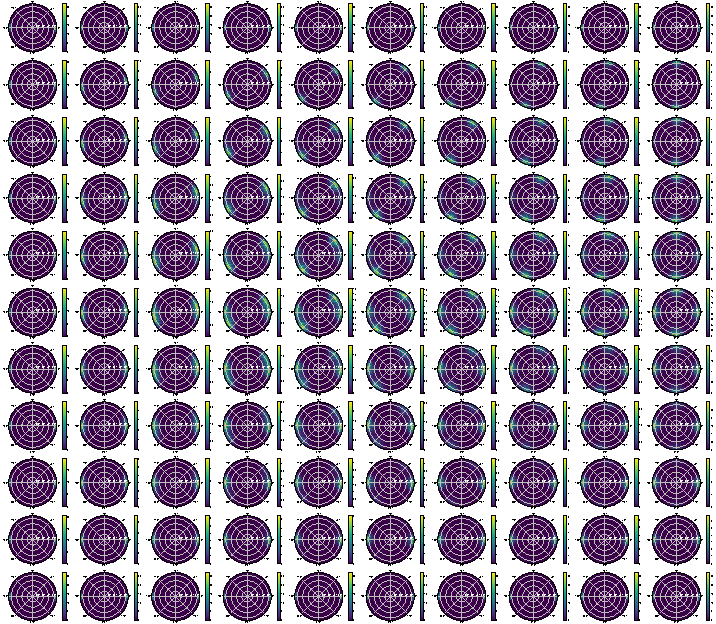
\includegraphics[width=1.0\textwidth]{gfx/model/results/histogram.pdf}};
% \begin{scope}[overlay]
%     \draw[->,thick] ($(image.north west)-(0.25,-0.25)$) -- ++(1,0) node [midway, above] {$\Omega$};
%     \draw[->,thick] ($(image.north west)-(0.25,-0.25)$) -- ++(0,-1) node [midway, above, rotate=90] {$\Psi$};
% \end{scope}
% \path ($(image.north west) + (-.5,.5)$) -- ($(image.north east) + (.5,.5)$);
% \end{tikzpicture}
% }
% \caption{Histogram cube\_2pop\_model}
% \label{app:model_histogram}
% \end{figure}
% %
% %
% \begin{figure}[!tb]
% \centering
% \resizebox{1.0\textwidth}{!}{
% \begin{tikzpicture}[>=latex]
% \node[inner sep=0pt] (image) at (0,0)
%     {\includegraphics[width=1.0\textwidth]{gfx/model/results/voxel_size_simulation_analysis.pdf}};
% \begin{scope}[overlay]
%     \draw[->,thick] ($(image.north west)-(0.25,-0.25)$) -- ++(1,0) node [midway, above] {$voxel_size$};
%     \draw[->,thick] ($(image.north west)-(0.25,-0.25)$) -- ++(0,-1) node [midway, above, rotate=90] {$f0_inc$};
% \end{scope}
% \path ($(image.north west) + (-.5,.5)$) -- ($(image.north east) + (.5,.5)$);
% \end{tikzpicture}
% }
% \vspace{-1ex}
% \begin{center}
% \begin{tikzpicture}
%     \draw[thin] (-3.0,-0.625) rectangle (3.0,0.25);
%     \draw [green!50!black] (-2.5,0) -- (-1.5,0) node [below, midway, black] {truth};
%     \draw [red,dashed] (-0.5,0) -- (0.5,0) node [below, midway, black] {model=r};
%     \draw [blue, dash dot] (1.5,0) -- (2.5,0) node [below, midway, black] {model=p};
% \end{tikzpicture}
% \end{center}
% \caption{voxel\_size\_5\_}
% \label{app:model_histogram}
% \end{figure}
% %
% \begin{figure}[!tb]
% \centering
% \resizebox{1.0\textwidth}{!}{
% \begin{tikzpicture}[>=latex]
% \node[inner sep=0pt] (image) at (0,0)
%     {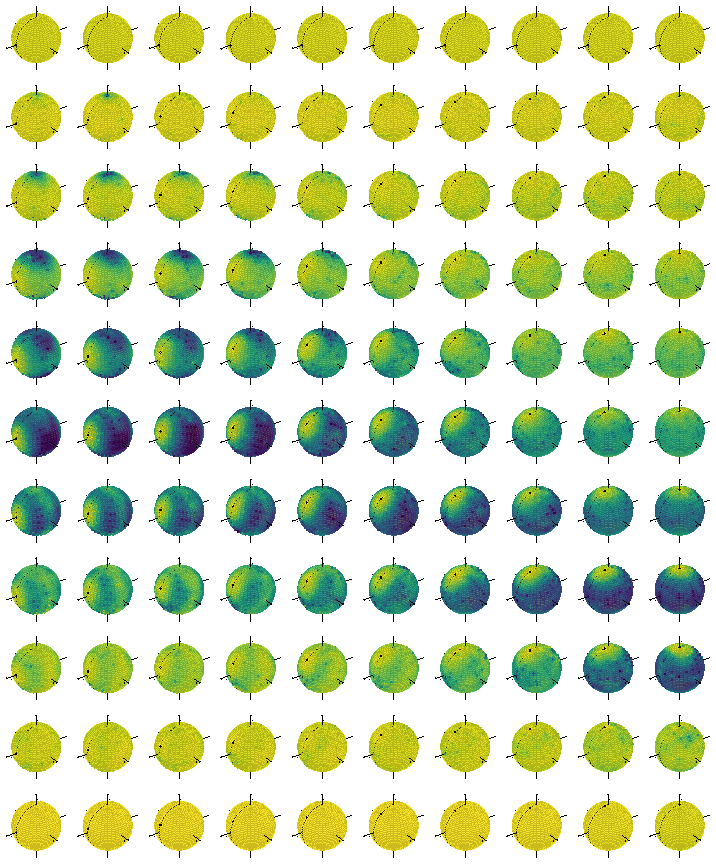
\includegraphics[width=1.0\textwidth]{gfx/simpli/results/simulation_analysis_spheres_LAP_p.pdf}};
% \begin{scope}[overlay]
%     \draw[->,thick] ($(image.north west)-(0.25,-0.25)$) -- ++(1,0) node [midway, above] {$\mathfrak{f}_0^\alpha$};
%     \draw[->,thick] ($(image.north west)-(0.25,-0.25)$) -- ++(0,-1) node [midway, above, rotate=90] {$\mathfrak{f}_0^\Psi$};
% \end{scope}
% \path ($(image.north west) + (-.5,.5)$) -- ($(image.north east) + (.5,.5)$);
% \end{tikzpicture}
% }
% \caption{Sphere LAP p}
% \label{app:model_histogram}
% \end{figure}
% %
% \begin{figure}[!tb]
% \centering
% \resizebox{1.0\textwidth}{!}{
% \begin{tikzpicture}[>=latex]
% \node[inner sep=0pt] (image) at (0,0)
%     {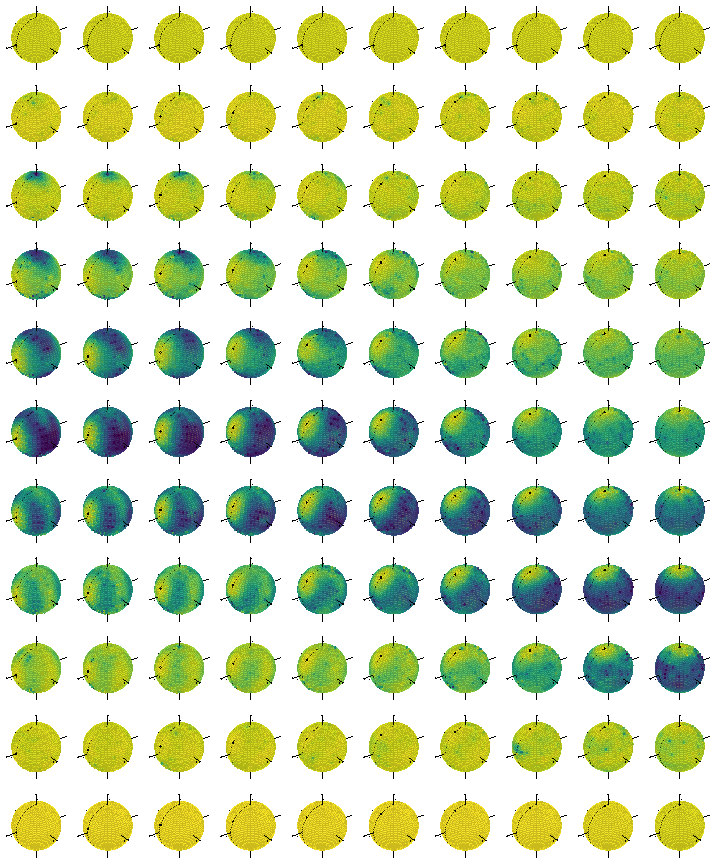
\includegraphics[width=1.0\textwidth]{gfx/simpli/results/simulation_analysis_spheres_LAP_r.pdf}};
% \begin{scope}[overlay]
%     \draw[->,thick] (image.north west) -- ++(1,0) node [midway, above] {$\alpha_0$};
%     \draw[->,thick] (image.north west) -- ++(0,-1) node [midway, above, rotate=90] {$\Psi_0$};
% \end{scope}
% \path ($(image.north west) + (-.5,.5)$) -- ($(image.north east) + (.5,.5)$);
% \end{tikzpicture}
% }
% \caption{Sphere LAP r}
% \label{app:model_histogram}
% \end{figure}
% %
% \begin{figure}[!tb]
% \centering
% \resizebox{1.0\textwidth}{!}{
% \begin{tikzpicture}[>=latex]
% \node[inner sep=0pt] (image) at (0,0)
%     {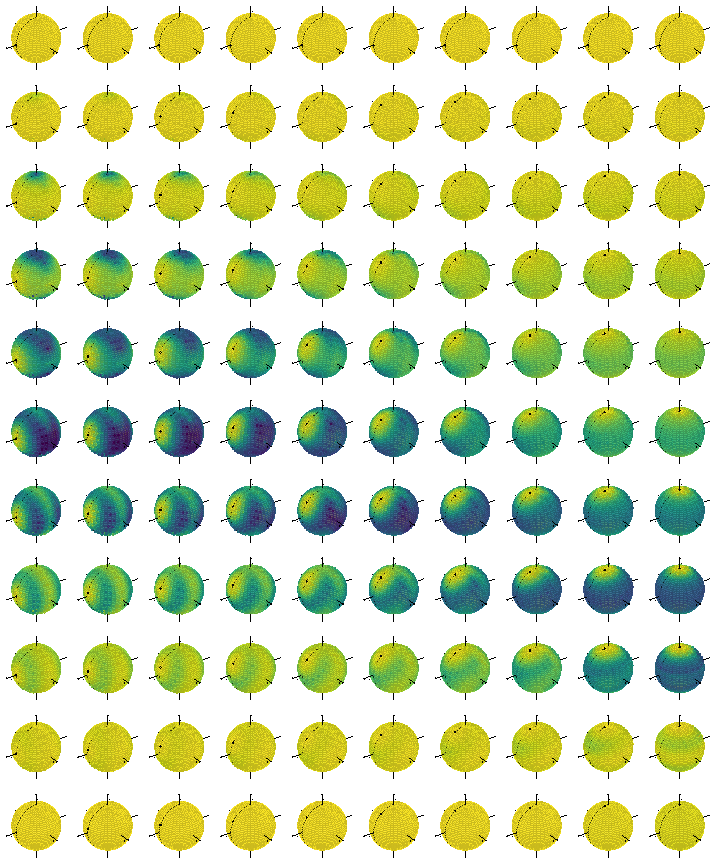
\includegraphics[width=1.0\textwidth]{gfx/simpli/results/simulation_analysis_spheres_PM_p.pdf}};
% \begin{scope}[overlay]
%     \draw[->,thick] ($(image.north west)-(0.25,-0.25)$) -- ++(1,0) node [midway, above] {$f_0$};
%     \draw[->,thick] ($(image.north west)-(0.25,-0.25)$) -- ++(0,-1) node [midway, above, rotate=90] {$\Psi$};
% \end{scope}
% \path ($(image.north west) + (-.5,.5)$) -- ($(image.north east) + (.5,.5)$);
% \end{tikzpicture}
% }
% \caption{Sphere PM p}
% \label{app:model_histogram}
% \end{figure}
% %
% \begin{figure}[!tb]
% \centering
% \resizebox{1.0\textwidth}{!}{
% \begin{tikzpicture}[>=latex]
% \node[inner sep=0pt] (image) at (0,0)
%     {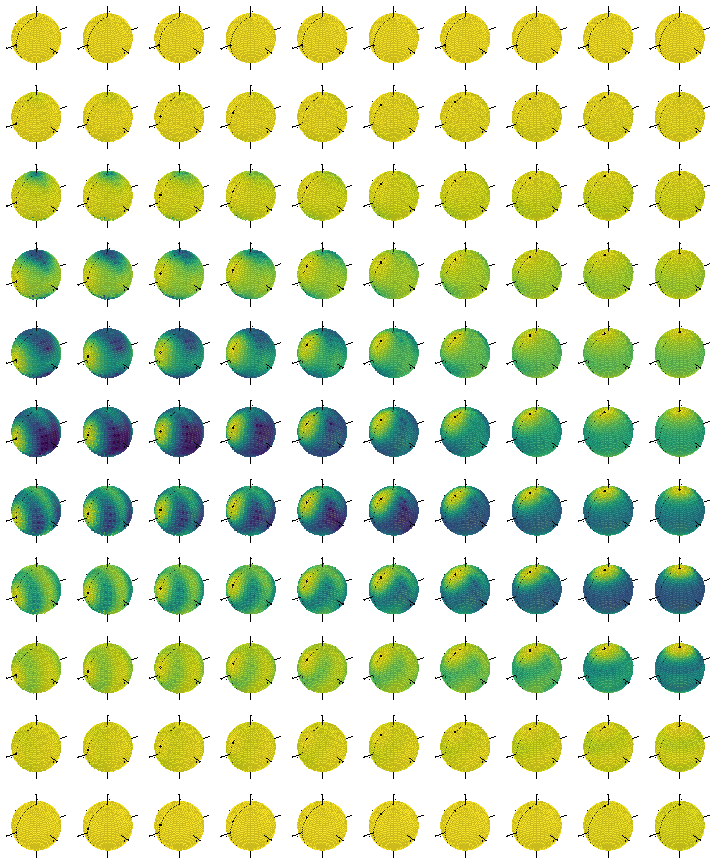
\includegraphics[width=1.0\textwidth]{gfx/simpli/results/simulation_analysis_spheres_PM_r.pdf}};
% \begin{scope}[overlay]
%     \draw[->,thick] ($(image.north west)-(0.25,-0.25)$) -- ++(1,0) node [midway, above] {$f_0$};
%     \draw[->,thick] ($(image.north west)-(0.25,-0.25)$) -- ++(0,-1) node [midway, above, rotate=90] {$\Psi$};
% \end{scope}
% \path ($(image.north west) + (-.5,.5)$) -- ($(image.north east) + (.5,.5)$);
% \end{tikzpicture}
% }
% \caption{Sphere PM r}
% \label{app:model_histogram}
% \end{figure}
% %
% \begin{figure}[!t]
% \centering
% \resizebox{1.0\textwidth}{!}{
% \includegraphics[width=\textwidth, page=2]{dev/rc1/cube_2pop_orientation_hist2d_output_cube_2pop_135_rc1.pdf}
% }
% \caption[Model orientation histograms]{density distribution of fiber segment orientation in initial and resulting models for $\fiberRadius = \SI{1}{\micro\meter}$. \itodo{fit ESAG} \ITODO{these are only resulting models!}}
% \label{app:modelOrientation}
% \end{figure}
% %
% %
%
\chapter{} % Model analysis
\label{app:modelAnalysis}
%
%
\fakesection{Model parameter}
%
\begin{figure}[!h]
    \centering
    \includegraphics[width=1\textwidth]{dev/rc1/mpara/pre_stats_box_plot_volume_output_parameter_statistic_rc1.pdf}
    \caption{Caption}
    \label{app:appModelVolumeBoxPlot}
\end{figure}
%
% % \foreach \n in {1,3,...,10}{
% % \begin{landscape}
% \begin{figure}[!t]
% \centering
% % \resizebox{\textwidth}{!}{
% \includegraphics[width=\textwidth,page=1]{dev/rc1/mpara/pre_stats_time_evolve_all_output_parameter_statistic_rc1.pdf}
% \includegraphics[width=\textwidth,page=2]{dev/rc1/mpara/pre_stats_time_evolve_all_output_parameter_statistic_rc1.pdf}
% \end{figure}
% % \end{landscape}
%
%
\fakesection{Time evolution}
%
\setlength{\tikzwidth}{\textwidth}
\begin{sidewaysfigure}[]
\centering
\includegraphics[height=\tikzwidth,page=1]{dev/rc1/mpara/pre_stats_time_evolve_all_output_parameter_statistic_rc1.pdf}
\includegraphics[height=\tikzwidth,page=2]{dev/rc1/mpara/pre_stats_time_evolve_all_output_parameter_statistic_rc1.pdf}
\label{app:pste1}
\end{sidewaysfigure}
%
\begin{sidewaysfigure}[]
\centering
% \resizebox{\tikzwidth}{!}{
\includegraphics[height=\tikzwidth,page=3]{dev/rc1/mpara/pre_stats_time_evolve_all_output_parameter_statistic_rc1.pdf}
\includegraphics[height=\tikzwidth,page=4]{dev/rc1/mpara/pre_stats_time_evolve_all_output_parameter_statistic_rc1.pdf}
% }
\label{app:pste2}
\end{sidewaysfigure}
%
\begin{sidewaysfigure}[]
\centering
% \resizebox{\textwidth}{!}{
\includegraphics[height=\tikzwidth,page=5]{dev/rc1/mpara/pre_stats_time_evolve_all_output_parameter_statistic_rc1.pdf}
\includegraphics[height=\tikzwidth,page=6]{dev/rc1/mpara/pre_stats_time_evolve_all_output_parameter_statistic_rc1.pdf}
\label{app:pste3}
\end{sidewaysfigure}
%
\begin{sidewaysfigure}[]
\centering
% \resizebox{\textwidth}{!}{
\includegraphics[height=\tikzwidth,page=7]{dev/rc1/mpara/pre_stats_time_evolve_all_output_parameter_statistic_rc1.pdf}
\includegraphics[height=\tikzwidth,page=8]{dev/rc1/mpara/pre_stats_time_evolve_all_output_parameter_statistic_rc1.pdf}
\label{app:pste4}
\end{sidewaysfigure}
%
\begin{sidewaysfigure}[]
\centering
% \resizebox{\textwidth}{!}{
\includegraphics[height=\tikzwidth,page=9]{dev/rc1/mpara/pre_stats_time_evolve_all_output_parameter_statistic_rc1.pdf}
\includegraphics[height=\tikzwidth,page=10]{dev/rc1/mpara/pre_stats_time_evolve_all_output_parameter_statistic_rc1.pdf}
\label{app:pste5}
\end{sidewaysfigure}
%
%
\fakesection{Histogramms}
%
\begin{figure}
    \centering
    \includegraphics[width=\textwidth, page=2]{dev/rc1/cube_2pop_orientation_hist2d_output_cube_2pop_135_rc1.pdf}
    \caption{Caption}
    \label{app:modelHistOrientation}
\end{figure}[]
%
\fakesection{Speedup}
%
\begin{figure}[!t]
\centering
\includegraphics[page=2]{dev/rc1/speed/boxplot_output_r_0.5.pkl_speedup.csv.pdf}
\caption[\code{model.Sovler} speedup]{\code{model.Sovler} speedup. The time measurements are taken after $\Delta_{\mathit{steps}}$ for the next $\SI{25}{\steps}$ for parallel $(||)$ and crossing $(\times)$ fiber configurations.}
\label{app:solverSpeedupAll}
\end{figure}
%
%
%
\fakesection{Simulation Library}
\begin{table}[htb]
\centering
\caption[Opening angle distribution]{Orientation statistic of simulation model library.}
\resizebox{\textwidth}{!}{
\pgfplotstabletypeset[%
    thesisTableStyle,
    columns={omega,psi,pop,incl_mean,incl_std,incl_25,incl_50,incl_75,phi_mean,phi_std,phi_25,phi_50,phi_75,mean,std,25,50,75},
    every head row/.style={
        before row={
            \toprule
        },
        after row={$\si{\degree}$ & & & $\si{\degree}$ & $\si{\degree}$ & $\si{\degree}$ & $\si{\degree}$ & $\si{\degree}$ & $\si{\degree}$ & $\si{\degree}$ & $\si{\degree}$ & $\si{\degree}$ & $\si{\degree}$ & $\si{\degree}$ & $\si{\degree}$ & $\si{\degree}$ & $\si{\degree}$ & $\si{\degree}$ \\ \midrule},
    },
    columns/omega/.style={column name=$\Omega$},
    columns/psi/.style={column name=$\Psi$},
    columns/mean/.style={column name=$<d\Omega>$,zerofill,precision=0},
    columns/std/.style={column name=$\sigma(d\Omega)$,zerofill,precision=0},
    columns/25/.style={column name=$25(d\Omega)$,zerofill,precision=0},
    columns/50/.style={column name=$50(d\Omega)$,zerofill,precision=0},
    columns/75/.style={column name=$75(d\Omega)$,zerofill,precision=0},
    columns/incl_mean/.style={column name=$<\alpha>$,fixed,fixed zerofill,precision=0},
    columns/incl_std/.style={column name=$\sigma(\alpha)$,fixed,fixed zerofill,precision=0},
    columns/incl_25/.style={column name=$25(\alpha)$,fixed,fixed zerofill,precision=0},
    columns/incl_50/.style={column name=$50(\alpha)$,fixed,fixed zerofill,precision=0},
    columns/incl_75/.style={column name=$75(\alpha)$,fixed,fixed zerofill,precision=0},
    columns/phi_mean/.style={column name=$<\varphi>$,fixed,fixed zerofill,precision=0},
    columns/phi_std/.style={column name=$\sigma(\varphi)$,fixed,fixed zerofill,precision=0},
    columns/phi_25/.style={column name=$25(\varphi)$,fixed,fixed zerofill,precision=0},
    columns/phi_50/.style={column name=$50(\varphi)$,fixed,fixed zerofill,precision=0},
    columns/phi_75/.style={column name=$75(\varphi)$,fixed,fixed zerofill,precision=0},
    col sep=comma,
    %
]
{dev/rc1/domega/omegas_ms_2pop.csv}
}
\label{app:modelDistribution}
\end{table}
%
% 
%
\chapter{}
\label{app:Simulation}
%
\fakesection{Tissue}
%
\begin{sidewaysfigure}[!p]
\resizebox{\textheight}{!}{
\begin{tabular}{cc}
\includegraphics[]{dev/rc1/tissue/bf_rc1_retardation_PM_Roden.pdf}&
\includegraphics[]{dev/rc1/tissue/bf_rc1_retardation_PM_Human.pdf}\\
\includegraphics[]{dev/rc1/tissue/bf_rc1_transmittance_PM_Roden.pdf}&
\includegraphics[]{dev/rc1/tissue/bf_rc1_transmittance_PM_Human.pdf}
\end{tabular}}
\end{sidewaysfigure}
%
\fakesection{Voxelsize}
%
\begin{figure}[!p]
% 2_simulation/0_parameter/fiber_radii.py
\centering
\includegraphics[width=\textwidth, page=1]{dev/rc1/voxel_size/voxel_size_plots_data_output_vs_135_0.01_6_25_vervet_r_rc1.pdf}
\caption[voxel size model with noise]{The mean difference is constant for smaller voxel sizes and does not start to grow significantly before $\voxels=\SI{0.125}{\micro\meter}$.}
\label{app:voxelsizeNoise}
\end{figure}
%
%
%
\fakesection{domega}
%
\begin{figure}[!t]
    \centering
    \includegraphics[]{dev/rc1/domega/cube_2pop_domega_analysis_all_output.pdf}
    \caption{Direction and inclination distribution of simulation model library.}
    % \label{fig:my_label}
\end{figure}
%
%
%
% %%%%%%%%%%%%%%%%%%%%%%%%%%%%%%%%%%%%%%%%%%%%%%%%%%%%%%%%%%%
% SINGLE
% %%%%%%%%%%%%%%%%%%%%%%%%%%%%%%%%%%%%%%%%%%%%%%%%%%%%%%%%%%%
%
\fakesection{Single fiber population}
%
\begin{figure}[!p]
\centering
% \begin{minipage}{0.45\textwidth}
\resizebox{\textwidth}{!}{
\rotatebox{90}{
\begin{tabular}{c|c}
\begin{tabular}{c|c}
    \includegraphics[]{dev/rc1/single/cube_2pop_135_rc1_single_plots_single_pop_hist_0.0.pdf} &
    \includegraphics[]{dev/rc1/single/cube_2pop_135_rc1_single_plots_single_pop_hist_25.0.pdf} \\
    \includegraphics[]{dev/rc1/single/cube_2pop_135_rc1_single_plots_single_pop_hist_5.0.pdf} &
    \includegraphics[]{dev/rc1/single/cube_2pop_135_rc1_single_plots_single_pop_hist_30.0.pdf} \\
    \includegraphics[]{dev/rc1/single/cube_2pop_135_rc1_single_plots_single_pop_hist_10.0.pdf} &
    \includegraphics[]{dev/rc1/single/cube_2pop_135_rc1_single_plots_single_pop_hist_35.0.pdf} \\
    \includegraphics[]{dev/rc1/single/cube_2pop_135_rc1_single_plots_single_pop_hist_15.0.pdf} &
    \includegraphics[]{dev/rc1/single/cube_2pop_135_rc1_single_plots_single_pop_hist_40.0.pdf} \\
    \includegraphics[]{dev/rc1/single/cube_2pop_135_rc1_single_plots_single_pop_hist_20.0.pdf} &
    \includegraphics[]{dev/rc1/single/cube_2pop_135_rc1_single_plots_single_pop_hist_45.0.pdf}
\end{tabular}
&
\begin{tabular}{c|c}
    \includegraphics[]{dev/rc1/single/cube_2pop_135_rc1_single_plots_single_pop_hist_50.0.pdf} &
    \includegraphics[]{dev/rc1/single/cube_2pop_135_rc1_single_plots_single_pop_hist_75.0.pdf} \\
    \includegraphics[]{dev/rc1/single/cube_2pop_135_rc1_single_plots_single_pop_hist_55.0.pdf} &
    \includegraphics[]{dev/rc1/single/cube_2pop_135_rc1_single_plots_single_pop_hist_80.0.pdf} \\
    \includegraphics[]{dev/rc1/single/cube_2pop_135_rc1_single_plots_single_pop_hist_60.0.pdf} &
    \includegraphics[]{dev/rc1/single/cube_2pop_135_rc1_single_plots_single_pop_hist_85.0.pdf} \\
    \includegraphics[]{dev/rc1/single/cube_2pop_135_rc1_single_plots_single_pop_hist_65.0.pdf} &
    \includegraphics[]{dev/rc1/single/cube_2pop_135_rc1_single_plots_single_pop_hist_90.0.pdf} \\
    \includegraphics[]{dev/rc1/single/cube_2pop_135_rc1_single_plots_single_pop_hist_70.0.pdf} &
\end{tabular}
\end{tabular}
}}
%
\caption[sim]{left: 2d log histogramm orientation from rofl analysis of simulation, right: 2d log histogramm of orientation of model segemnts. \itodo{rfc plots}}
\label{app:single_fiber_pop_hist_app}
\end{figure}
%
%
% %%%%%%%%%%%%%%%%%%%%%%%%%%%%%%%%%%%%%%%%%%%%%%%%%%%%%%%%%%%
% FLAT
% %%%%%%%%%%%%%%%%%%%%%%%%%%%%%%%%%%%%%%%%%%%%%%%%%%%%%%%%%%%
%
\fakesection{Crossing fiber population}
%
\begin{figure}[!p]
\centering
\setlength{\tikzwidth}{0.45\textwidth}
\begin{tabular}{c|c}
    \includegraphics[width=\tikzwidth]{dev/rc1/flat/cube_2pop_135_rc1_flat_plots_flat_pop_hist_omega_0.0_psi_0.3.pdf} &
    \includegraphics[width=\tikzwidth]{dev/rc1/flat/cube_2pop_135_rc1_flat_plots_flat_pop_hist_omega_50.0_psi_0.3.pdf} \\
    \includegraphics[width=\tikzwidth]{dev/rc1/flat/cube_2pop_135_rc1_flat_plots_flat_pop_hist_omega_10.0_psi_0.3.pdf} &
    \includegraphics[width=\tikzwidth]{dev/rc1/flat/cube_2pop_135_rc1_flat_plots_flat_pop_hist_omega_60.0_psi_0.3.pdf} \\
    \includegraphics[width=\tikzwidth]{dev/rc1/flat/cube_2pop_135_rc1_flat_plots_flat_pop_hist_omega_20.0_psi_0.3.pdf} &
    \includegraphics[width=\tikzwidth]{dev/rc1/flat/cube_2pop_135_rc1_flat_plots_flat_pop_hist_omega_70.0_psi_0.3.pdf} \\
    \includegraphics[width=\tikzwidth]{dev/rc1/flat/cube_2pop_135_rc1_flat_plots_flat_pop_hist_omega_30.0_psi_0.3.pdf} &
    \includegraphics[width=\tikzwidth]{dev/rc1/flat/cube_2pop_135_rc1_flat_plots_flat_pop_hist_omega_80.0_psi_0.3.pdf} \\
    \includegraphics[width=\tikzwidth]{dev/rc1/flat/cube_2pop_135_rc1_flat_plots_flat_pop_hist_omega_40.0_psi_0.3.pdf} &
    \includegraphics[width=\tikzwidth]{dev/rc1/flat/cube_2pop_135_rc1_flat_plots_flat_pop_hist_omega_90.0_psi_0.3.pdf}
\end{tabular}
%
\caption[sim]{psi=0.3; left: 2d log histogramm orientation from rofl analysis of simulation, right: 2d log histogram of orientation of model segemnts. \itodo{legende}}
\label{app:flat_03_fiber_pop_hist}
\end{figure}
%
%
%
%
\begin{figure}[!p]
\centering
\setlength{\tikzwidth}{0.45\textwidth}
\begin{tabular}{c|c}
    \includegraphics[width=\tikzwidth]{dev/rc1/flat/cube_2pop_135_rc1_flat_plots_flat_pop_hist_omega_0.0_psi_0.5.pdf} &
    \includegraphics[width=\tikzwidth]{dev/rc1/flat/cube_2pop_135_rc1_flat_plots_flat_pop_hist_omega_50.0_psi_0.5.pdf} \\
    \includegraphics[width=\tikzwidth]{dev/rc1/flat/cube_2pop_135_rc1_flat_plots_flat_pop_hist_omega_10.0_psi_0.5.pdf} &
    \includegraphics[width=\tikzwidth]{dev/rc1/flat/cube_2pop_135_rc1_flat_plots_flat_pop_hist_omega_60.0_psi_0.5.pdf} \\
    \includegraphics[width=\tikzwidth]{dev/rc1/flat/cube_2pop_135_rc1_flat_plots_flat_pop_hist_omega_20.0_psi_0.5.pdf} &
    \includegraphics[width=\tikzwidth]{dev/rc1/flat/cube_2pop_135_rc1_flat_plots_flat_pop_hist_omega_70.0_psi_0.5.pdf} \\
    \includegraphics[width=\tikzwidth]{dev/rc1/flat/cube_2pop_135_rc1_flat_plots_flat_pop_hist_omega_30.0_psi_0.5.pdf} &
    \includegraphics[width=\tikzwidth]{dev/rc1/flat/cube_2pop_135_rc1_flat_plots_flat_pop_hist_omega_80.0_psi_0.5.pdf} \\
    \includegraphics[width=\tikzwidth]{dev/rc1/flat/cube_2pop_135_rc1_flat_plots_flat_pop_hist_omega_40.0_psi_0.5.pdf} &
    \includegraphics[width=\tikzwidth]{dev/rc1/flat/cube_2pop_135_rc1_flat_plots_flat_pop_hist_omega_90.0_psi_0.5.pdf}
\end{tabular}
%
\caption[sim]{psi=0.5; left: 2d log histogramm orientation from rofl analysis of simulation, right: 2d log histogramm of orientation of model segemnts. \itodo{legende}}
\label{app:flat_05_fiber_pop_hist}
\end{figure}
%
%
%
\begin{figure}[!p]
\centering
\resizebox{\textwidth}{!}{
\begin{tabular}{cc}
\includegraphics[page=1]{dev/rc1/analysis/plots_flat_pop_output_cube_2pop_135_rc1_flat.pdf} &
\includegraphics[page=2]{dev/rc1/analysis/plots_flat_pop_output_cube_2pop_135_rc1_flat.pdf}\\
\includegraphics[page=3]{dev/rc1/analysis/plots_flat_pop_output_cube_2pop_135_rc1_flat.pdf} &
\includegraphics[page=4]{dev/rc1/analysis/plots_flat_pop_output_cube_2pop_135_rc1_flat.pdf}
\end{tabular}
}
\end{figure}
%
\begin{figure}[!p]
\centering
\resizebox{\textwidth}{!}{
\begin{tabular}{cc}
\includegraphics[page=5]{dev/rc1/analysis/plots_flat_pop_output_cube_2pop_135_rc1_flat.pdf} &
\includegraphics[page=6]{dev/rc1/analysis/plots_flat_pop_output_cube_2pop_135_rc1_flat.pdf}\\
\includegraphics[page=7]{dev/rc1/analysis/plots_flat_pop_output_cube_2pop_135_rc1_flat.pdf} &
\includegraphics[page=8]{dev/rc1/analysis/plots_flat_pop_output_cube_2pop_135_rc1_flat.pdf}
\end{tabular}
}
\end{figure}
%
\begin{figure}[]
\centering
\resizebox{\textwidth}{!}{
\begin{tabular}{cc}
\includegraphics[page=9]{dev/rc1/analysis/plots_flat_pop_output_cube_2pop_135_rc1_flat.pdf} &
\includegraphics[page=10]{dev/rc1/analysis/plots_flat_pop_output_cube_2pop_135_rc1_flat.pdf}
\end{tabular}
}
\end{figure}
%
%
% %%%%%%%%%%%%%%%%%%%%%%%%%%%%%%%%%%%%%%%%%%%%%%%%%%%%%%%%%%%
% INCLINED
% %%%%%%%%%%%%%%%%%%%%%%%%%%%%%%%%%%%%%%%%%%%%%%%%%%%%%%%%%%%
%
\fakesection{Inclined fiber population}
%
\begin{figure}[!p]
\centering
\setlength{\tikzwidth}{0.45\textwidth}
\begin{tabular}{c|c}
    \includegraphics[width=\tikzwidth]{dev/rc1/inclined/cube_2pop_135_rc1_inclined_plots_inclined_pop_hist_omega_0.0_psi_0.3.pdf} &
    \includegraphics[width=\tikzwidth]{dev/rc1/inclined/cube_2pop_135_rc1_inclined_plots_inclined_pop_hist_omega_50.0_psi_0.3.pdf} \\ \includegraphics[width=\tikzwidth]{dev/rc1/inclined/cube_2pop_135_rc1_inclined_plots_inclined_pop_hist_omega_10.0_psi_0.3.pdf} & \includegraphics[width=\tikzwidth]{dev/rc1/inclined/cube_2pop_135_rc1_inclined_plots_inclined_pop_hist_omega_60.0_psi_0.3.pdf} \\
    \includegraphics[width=\tikzwidth]{dev/rc1/inclined/cube_2pop_135_rc1_inclined_plots_inclined_pop_hist_omega_20.0_psi_0.3.pdf} &
    \includegraphics[width=\tikzwidth]{dev/rc1/inclined/cube_2pop_135_rc1_inclined_plots_inclined_pop_hist_omega_70.0_psi_0.3.pdf} \\ \includegraphics[width=\tikzwidth]{dev/rc1/inclined/cube_2pop_135_rc1_inclined_plots_inclined_pop_hist_omega_30.0_psi_0.3.pdf} & \includegraphics[width=\tikzwidth]{dev/rc1/inclined/cube_2pop_135_rc1_inclined_plots_inclined_pop_hist_omega_80.0_psi_0.3.pdf} \\
    \includegraphics[width=\tikzwidth]{dev/rc1/inclined/cube_2pop_135_rc1_inclined_plots_inclined_pop_hist_omega_40.0_psi_0.3.pdf} &
    \includegraphics[width=\tikzwidth]{dev/rc1/inclined/cube_2pop_135_rc1_inclined_plots_inclined_pop_hist_omega_90.0_psi_0.3.pdf}
\end{tabular}
%
\caption[sim]{psi=0.3; left: 2d log histogramm orientation from rofl analysis of simulation, right: 2d log histogram of orientation of model segemnts. \itodo{legende}}
\label{app:incl_03_fiber_pop_hist}
\end{figure}
%
%
%
%
\begin{figure}[!p]
\centering
\setlength{\tikzwidth}{0.45\textwidth}
\begin{tabular}{c|c}
    \includegraphics[width=\tikzwidth]{dev/rc1/inclined/cube_2pop_135_rc1_inclined_plots_inclined_pop_hist_omega_0.0_psi_0.5.pdf} &
    \includegraphics[width=\tikzwidth]{dev/rc1/inclined/cube_2pop_135_rc1_inclined_plots_inclined_pop_hist_omega_50.0_psi_0.5.pdf} \\
    \includegraphics[width=\tikzwidth]{dev/rc1/inclined/cube_2pop_135_rc1_inclined_plots_inclined_pop_hist_omega_10.0_psi_0.5.pdf} &
    \includegraphics[width=\tikzwidth]{dev/rc1/inclined/cube_2pop_135_rc1_inclined_plots_inclined_pop_hist_omega_60.0_psi_0.5.pdf} \\
    \includegraphics[width=\tikzwidth]{dev/rc1/inclined/cube_2pop_135_rc1_inclined_plots_inclined_pop_hist_omega_20.0_psi_0.5.pdf} &
    \includegraphics[width=\tikzwidth]{dev/rc1/inclined/cube_2pop_135_rc1_inclined_plots_inclined_pop_hist_omega_70.0_psi_0.5.pdf} \\
    \includegraphics[width=\tikzwidth]{dev/rc1/inclined/cube_2pop_135_rc1_inclined_plots_inclined_pop_hist_omega_30.0_psi_0.5.pdf} &
    \includegraphics[width=\tikzwidth]{dev/rc1/inclined/cube_2pop_135_rc1_inclined_plots_inclined_pop_hist_omega_80.0_psi_0.5.pdf} \\
    \includegraphics[width=\tikzwidth]{dev/rc1/inclined/cube_2pop_135_rc1_inclined_plots_inclined_pop_hist_omega_40.0_psi_0.5.pdf} &
    \includegraphics[width=\tikzwidth]{dev/rc1/inclined/cube_2pop_135_rc1_inclined_plots_inclined_pop_hist_omega_90.0_psi_0.5.pdf}
\end{tabular}
%
\caption[sim]{psi=0.5; left: 2d log histogramm orientation from rofl analysis of simulation, right: 2d log histogramm of orientation of model segemnts. \itodo{legende}}
\label{app:incl_05_fiber_pop_hist}
\end{figure}
%
%
%
\begin{figure}[!p]
\centering
\resizebox{\textwidth}{!}{
\begin{tabular}{cc}
\includegraphics[page=1]{dev/rc1/analysis/plots_inclined_pop_output_cube_2pop_135_rc1_inclined.pdf} &
\includegraphics[page=2]{dev/rc1/analysis/plots_inclined_pop_output_cube_2pop_135_rc1_inclined.pdf}\\
\includegraphics[page=3]{dev/rc1/analysis/plots_inclined_pop_output_cube_2pop_135_rc1_inclined.pdf} &
\includegraphics[page=4]{dev/rc1/analysis/plots_inclined_pop_output_cube_2pop_135_rc1_inclined.pdf}
\end{tabular}
}
\end{figure}
%
\begin{figure}[!p]
\centering
\resizebox{\textwidth}{!}{
\begin{tabular}{cc}
\includegraphics[page=5]{dev/rc1/analysis/plots_inclined_pop_output_cube_2pop_135_rc1_inclined.pdf} &
\includegraphics[page=6]{dev/rc1/analysis/plots_inclined_pop_output_cube_2pop_135_rc1_inclined.pdf}\\
\includegraphics[page=7]{dev/rc1/analysis/plots_inclined_pop_output_cube_2pop_135_rc1_inclined.pdf} &
\includegraphics[page=8]{dev/rc1/analysis/plots_inclined_pop_output_cube_2pop_135_rc1_inclined.pdf}
\end{tabular}
}
\end{figure}
%
\begin{figure}[!p]
\centering
\resizebox{\textwidth}{!}{
\begin{tabular}{cc}
\includegraphics[page=9]{dev/rc1/analysis/plots_inclined_pop_output_cube_2pop_135_rc1_inclined.pdf} &
\includegraphics[page=10]{dev/rc1/analysis/plots_inclined_pop_output_cube_2pop_135_rc1_inclined.pdf}
\end{tabular}
}
\end{figure}
%
% %
% %
%
% \newpage
% \mbox{}
%
% **************************************************
% End of Document CONTENT
% **************************************************
\end{document}
